\documentclass[journal]{IEEEtran}
\usepackage[a5paper, margin=10mm]{geometry}
%\usepackage{lmodern} % Ensure lmodern is loaded for pdflatex
\usepackage{tfrupee} % Include tfrupee package


\setlength{\headheight}{1cm} % Set the height of the header box
\setlength{\headsep}{0mm}     % Set the distance between the header box and the top of the text


%\usepackage[a5paper, top=10mm, bottom=10mm, left=10mm, right=10mm]{geometry}

%
\usepackage{gvv-book}
\usepackage{gvv}
%\setlength{\intextsep}{10pt} % Space between text and floats

\makeindex

\begin{document}
\bibliographystyle{IEEEtran}
\onecolumn


\title{
	%\begin{flushleft}
	\begin{center}
	%MATRICES \\ In Geometry
	Trigonometry through Geometry
	\\
\rule{0.4\columnwidth}{0.4pt}
%\end{flushleft}
\end{center}
}
\author{
\vspace{11cm}
	%\begin{flushleft}
	\begin{center}
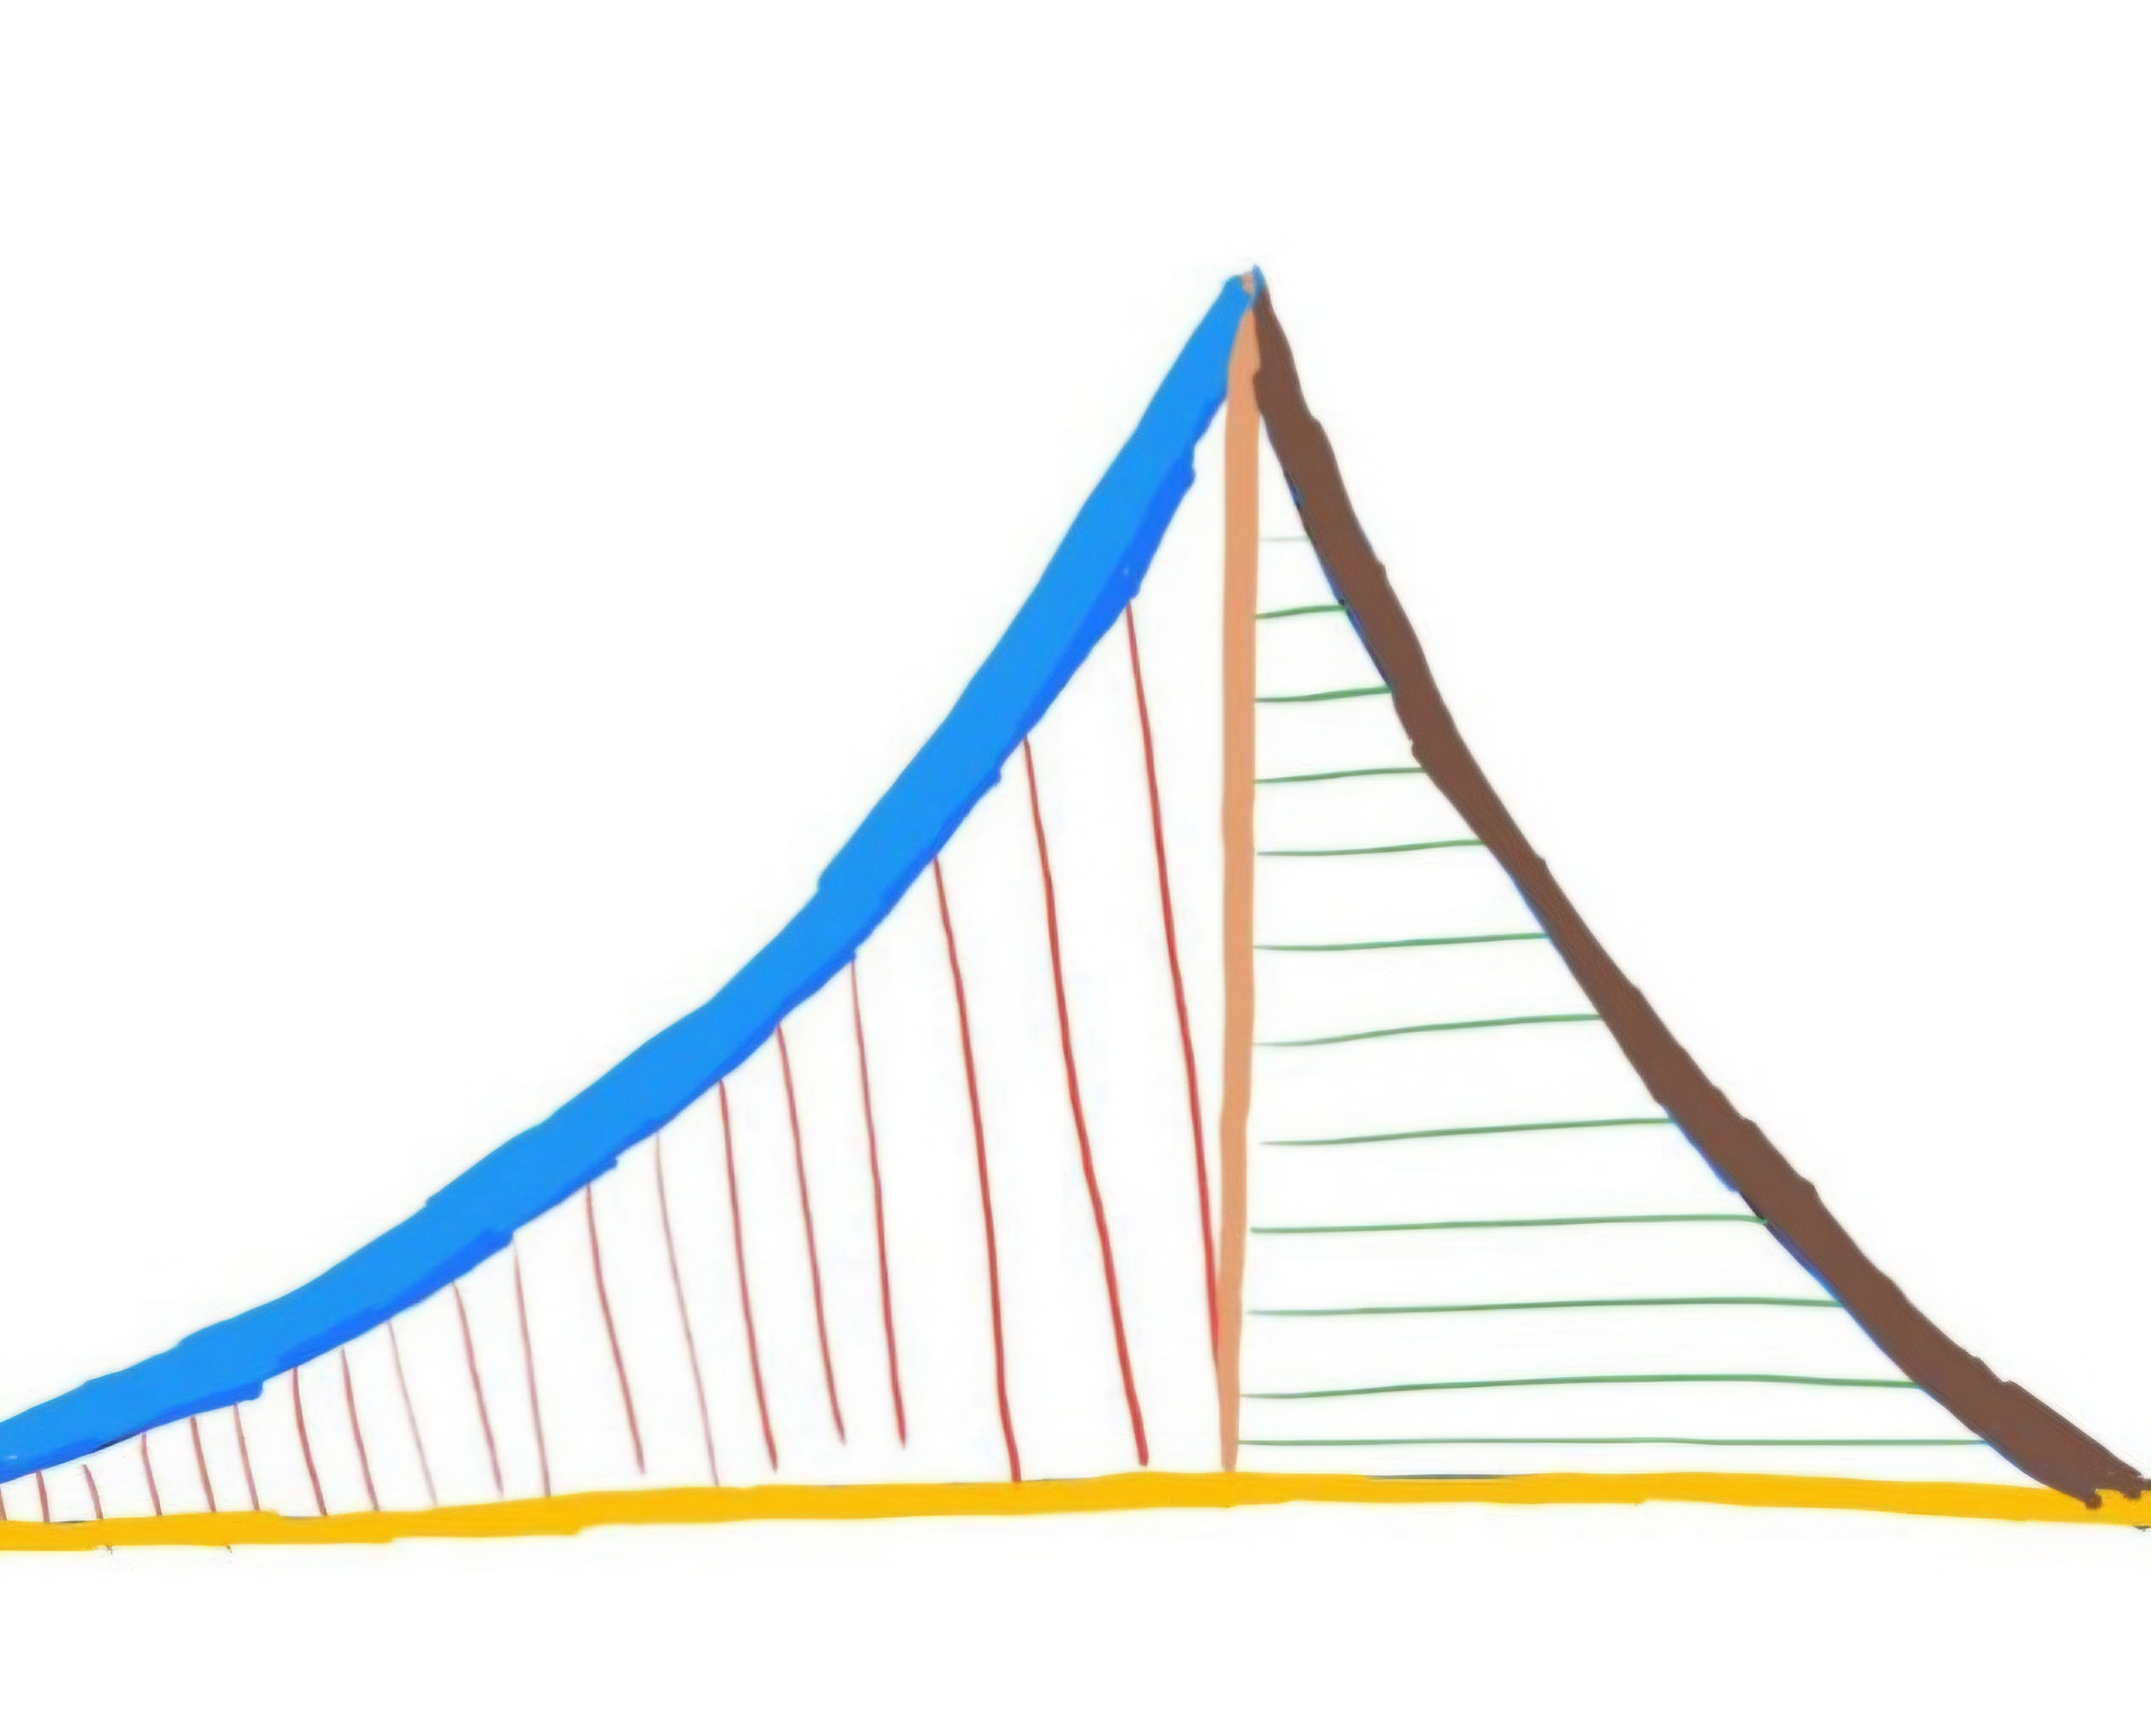
\includegraphics[width=0.2\columnwidth]{figs/logo.jpg}
\\
		{	\huge G. V. V. Sharma}
	\end{center}
	%\end{flushleft}
%\IEEEpubid{\makebox[\columnwidth]{978-1-7281-5966-1/20/\$31.00 ©2020 IEEE \hfill} \hspace{\columnsep}\makebox[\columnwidth]{ }}
}
\maketitle

\newpage
\section*{About this Book}

This book introduces trigonometry through high school geometry. This approach relies more on trigonometric equations than cumbersome constructions which are usually non intuitive.
 All problems in the book are from NCERT mathematics textbooks from Class 9-12.  Exercises are from CBSE board exam papers.   

The content is sufficient for all practical applications of trigonometry.
There is no copyright, so readers are free to print and share.  

This book is dedicated to my high school maths teacher, Dr. G.N. Chandwani. 
\begin{flushright}
\today
\end{flushright}
Github: https://github.com/gadepall/matgeo
		\\
License: https://creativecommons.org/licenses/by-sa/3.0/
\\
and
\\
https://www.gnu.org/licenses/fdl-1.3.en.html

\newpage


\tableofcontents

\newpage
%\twocolumn
\onecolumn


%\renewcommand{\theequation}{\theenumi}
\numberwithin{equation}{enumi}
\numberwithin{figure}{enumi}
%\renewcommand{\thefigure}{\theenumi}
\renewcommand{\thetable}{\theenumi}

\section{Triangle}
\subsection{Formulae}
\begin{enumerate}[label=\thesubsection.\arabic*.,ref=\thesubsection.\theenumi]
	\item 
A right angled triangle looks like Fig. \ref{fig:tri_right_angle}.
\begin{figure}[!ht]
\centering
\resizebox{0.75\columnwidth}{!}{%Code by GVV Sharma
%December 6, 2019
%released under GNU GPL
%Drawing a right angled triangle

\begin{tikzpicture}[scale=2]

%Triangle sides
\def\a{4}
\def\c{3}

%Marking coordiantes
\coordinate [label=above:$A$] (A) at (0,\c);
\coordinate [label=left:$B$] (B) at (0,0);
\coordinate [label=right:$C$] (C) at (\a,0);

%Drawing triangle ABC
\draw (A) -- node[left] {$\textrm{c}$} (B) -- node[below] {$\textrm{a}$} (C) -- node[above,,xshift=2mm] {$\textrm{b}$} (A);

%Drawing and marking angles

\tkzMarkAngle[color=red, fill=red!40,size=0.3](A,C,B)
\tkzMarkRightAngle[fill=blue!20,size=.3](A,B,C)
\tkzLabelAngle[pos=0.65](A,C,B){$\theta$}
\end{tikzpicture}
}
\caption{Right Angled Triangle}
\label{fig:tri_right_angle}	
\end{figure}
with angles $\angle A,\angle B$ and $\angle C$ and sides $a, b$ and $c$.  The unique feature of this triangle is $\angle B$ which is defined to be $90\degree$.
\item
	For simplicity, let the greek letter $\theta = \angle C$.  We have the following definitions.
\begin{equation}
\label{eq:tri_trig_defs}
\begin{matrix}
	\sin \theta = \frac{c}{b} & 	\cos \theta = \frac{a}{b} \\[1ex]
	\tan \theta = \frac{c}{a} & \cot \theta = \frac{1}{\tan \theta} \\[1ex]
	\csc \theta = \frac{1}{\sin \theta} & \sec \theta = \frac{1}{\cos \theta}
	\end{matrix}
\end{equation}
\item  
	\begin{equation}
	\cos \theta = \sin \brak{90\degree - \theta}
	\label{eq:tri_baudh_comp}	
	\end{equation}
\end{enumerate}

\subsection{Problems}
\begin{enumerate}[label=\thesubsection.\arabic*.,ref=\thesubsection.\theenumi]
\item $ABCD$ is a trapezium in which $AB  \parallel  DC$ and its diagonals intersect each other at the point $O$. Show
that
$\frac{AO}{ BO}=\frac{CO}{  DO}$
\item In an isosceles $\triangle ABC$, with $AB = AC$, the bisectors of $\angle B$ and $\angle C$ intersect each other at $O$. Join $A$ to $O$. Show that :
\begin{enumerate} 
\item $OB = OC$ 
\item $AO$ bisects $\angle A$
\end{enumerate}
\item $ABC$ is an isosceles triangle in which altitudes $BE$ and $CF$ are drawn to equal sides $AC$ and $AB$ respectively . Show that these altitudes are equal.
%
\item $ABC$ is a triangle in which altitudes $BE$ and $CF$ to sides $AC$ and $AB$ are equal. Show that
%
\begin{enumerate} 
\item $\triangle  ABE \cong  \triangle  ACF $
\item  $AB = AC$, i.e., $ABC$ is an isosceles triangle.
\end{enumerate}
\item $ABCD$ is a trapezium in which $AB  \parallel  DC$ and its diagonals intersect each other at the point $O$. Show
that
$\frac{AO}{ BO}=\frac{CO}{  DO}$
%
\item  $D$ is a point on the side $BC$ of a $\triangle ABC$ such that  $\angle  ADC =  \angle  BAC$. Show that $CA^2 = CB.CD$.
%
\item $BL$ and $CM$ are medians of a $\triangle ABC$ right angled at $A$. Prove that $4 (BL^2 + CM^2
) = 5 BC^2$ .
\item $O$ is any point inside a rectangle $ABCD$. Prove that $OB^2+OD^2 = OA^2+OC^2$.
\item   $D$ is a point on side $BC$ of  $\triangle  ABC$ such that
$\frac{BD}{CD}= \frac{AB}{AC}  $.  Prove that $AD$ is the bisector of  $\angle  BAC$.
\item $\vec{Q}$ is a point on the side $\vec{SR}$ of $\triangle \vec{PSR}$ such that $\vec{PQ=PR}$. Prove that $\vec{PS>PQ}$.
\item $\vec{S}$ is any point on side $\vec{QR}$ of a $\triangle \vec{PQR}$. Show that $\vec{PQ+QR+RP>2PS}$.
\item $\vec{D}$ is any point on side $\vec{AC}$ of a $\triangle \vec{ABC}$ with $\vec{AB=AC}$. Show that $\vec{CD<BD}$.
\item $AD$ is the bisector of $\angle BAC$. Prove that $AB>BD$.
\item Prove that sum of any two sides of a triangle is greater than twice the median with respect to the third side.
\item Prove that in a triangle, other than an equilateral triangle, angle opposite the longest side is greater than $\frac{2}{3}$ of a right angle.
\item P is a point in the interior of a parallelogram $ABCD$. Show that
\begin{enumerate}
\item $ar (APB) + ar (PCD) = \frac{1}{ 2}ar (ABCD)$
\item $ar (APD) + ar (PBC) = ar (APB) + ar (PCD)$
\end{enumerate}
%
\item $PQRS$ and $ABRS$ are parallelograms and $X$ is any point on side $BR$. show that 
\begin{enumerate} 
\item $ar (PQRS) = ar (ABRS)$
\item $ar (AX S) = \frac{1}{ 2} ar (PQRS)$
\end{enumerate}
\item $ABCD$ is a quadrilateral and $BE  \parallel  AC$ and also $BE$ meets $DC$ produced at $E$. Show that area of $ \triangle  ADE$ is equal to the area of the quadrilateral $ABCD$.
%
\item $E$ is any point on median $AD$ of a  $\triangle  ABC$. Show that $ar (ABE) = ar (ACE)$.
\item  In a $\triangle ABC, E$ is the mid-point of median $AD$. Show that $ar (BED) = \frac{1}{ 4}ar(ABC)$ .
%
\item AB is a diameter of the circle, $CD$ is a chord equal to the radius of the circle. $AC$ and $BD$ when extended intersect at a point $E$. Prove that $\angle AEB = 60\degree$.
\item If the non-parallel sides of a trapezium are equal, prove that it is cyclic.
\item Prove that the line of centres of two intersecting circles subtends equal angles at the
two points of intersection.
%
\end{enumerate}

\section{Applications}
\begin{enumerate}[label=\thesubsection.\arabic*.,ref=\thesubsection.\theenumi]
\item A ladder is placed against a wall such that its foot is at a distance of 2.5 m from the wall and its top reaches a window 6 m above the ground. Find the length of the ladder.
\item  A ladder 10 m long reaches a window 8 m above the ground. Find the distance of the foot of the ladder from base of the wall.
\item  A guy wire attached to a vertical pole of height 18 m is 24 m long and has a stake attached to the other end. How far from the base of the pole should the stake be driven so that the wire will be taut?
\item  An aeroplane leaves an airport and flies due north at a speed of 1000 km per hour. At the same time, another aeroplane leaves the same airport and flies due west at a speed of 1200 km per hour. How far apart will be the two planes after $1\frac{1}{2}$ hours?
\item  Two poles of heights 6 m and 11 m stand on a plane ground. If the distance between the feet of the poles is 12 m, find the distance between their tops.
\item  In  $\triangle  ABC, AB = 6\sqrt{3} cm, AC = 12 cm$ and $BC = 6 cm$. Find the angle $B$.
\item An aircraft is flying at a height of 3400 m above the ground. If the angle subtended at a ground observation point by the aircraft positions 10.0 s apart is 30$\degree$, what is the speed of the aircraft ?
%
\item A statue, 1.6 m tall, stands on the top of a pedestal. From a point on the ground, the angle of elevation of the top of the statue is 60$\degree$ and from the same point the angle of elevation of the top of the pedestal is 45$\degree$. Find the height of the pedestal.
\item The angle of elevation of the top of a building from the foot of the tower is 30$\degree$ and the angle of elevation of the top of the tower from the foot of the building is 60$\degree$. If the tower is 50 m high, find the height of the building.
\item Two poles of equal heights are standing opposite each other on either side of the road, which is 80 m wide. From a point between them on the road, the angles of elevation of the top of the poles are 60$\degree$ and 30$\degree$, respectively. Find the height of the poles and the distances of the point from the poles.
\item A TV tower stands vertically on a bank of a canal. From a point on the other bank directly opposite the tower, the angle of elevation of the top of the tower is 60$\degree$. From another point 20 m away from this point on the line joing this point to the foot of the tower, the angle of elevation of the top of the tower is 30$\degree$. Find the height of the tower and the width of the canal.
\item From the top of a 7 m high building, the angle of elevation of the top of a cable tower is 60$\degree$ and the angle of depression of its foot is 45$\degree$. Determine the height of the tower.
\item As observed from the top of a 75 m high lighthouse from the sea-level, the angles of depression of two ships are 30$\degree$ and 45$\degree$. If one ship is exactly behind the other on the same side of the lighthouse, find the distance between the two ships.
\item A 1.2 m tall girl spots a balloon moving with the wind in a horizontal line at a height of 88.2 m from the ground. The angle of elevation of the balloon from the eyes of the girl at any instant is 60$\degree$. After some time, the angle of elevation reduces to 30$\degree$. Find the distance travelled by the balloon during the interval.
\item A straight highway leads to the foot of a tower. A man standing at the top of the tower observes a car at an angle of depression of 30$\degree$, which is approaching the foot of the tower with a uniform speed. Six seconds later, the angle of depression of the car is found to be 60$\degree$. Find the time taken by the car to reach the foot of the tower from this point.
\item The angles of elevation of the top of a tower from two points at a distance of 4 m and 9 m from the base of the tower and in the same straight line with it are complementary. Prove that the height of the tower is 6 m.
\item A girl of height 90 cm is walking away from the base of a lamp-post at a speed of 1.2 m/s. If the lamp is 3.6 m above the ground, find the length of her shadow after 4 seconds.
\item  Nazima is fly fishing in a stream. The tip of her fishing rod is 1.8 m above the surface of the water and the fly at the end of the string rests on the water 3.6 m away and 2.4 m from a point directly under the tip of the rod. Assuming that her string (from the tip of her rod to the fly) is taut, how much string does she have out? If she pulls in the string at the rate of 5 cm per second, what will be the horizontal distance of the fly from her after 12 seconds?
%
\item  A vertical pole of length 6 m casts a shadow 4 m long on the ground and at the same time a tower casts a shadow 28 m long. Find the height of the tower.
\item A circus artist is climbing a 20m long rope, which is tightly stretched and tied from the top of a vertical pole to the ground.  Find the height of the pole, if the angle made by the rope with the ground level is 30$\degree$.
%
\item A tree breaks due to storm and the broken part bends so that the top of the tree touches the ground making an angle of 30$\degree$ with it.  The distance between the foot of the tree to the point where the top touches the ground is 8m.  Find the height of the tree.
%
\item A contractor plans to install two slides for the children to play in a park.  For the children below the age of 5 years, she prefers to have a slide whose top is at a height of 1.5m, and is inclined at an angle of 30$\degree$  to the ground, whereas for elder children she wants to have a steep slide at a height of 3m, and inclined at an angle of 60$\degree$ to the ground.  What should be the length of the slide in each case?
%
\item The angle of elevation of the top of a tower from a point on the ground, which is 30m away from the foot of the tower, is 30$\degree$.  Find the height of the tower.
%
\item A kite is flying at a height of 60m above the ground.  The string attached to the kite is temporarily tied to a point on the ground.  The inclination of the string with the ground is $60\degree$.  Find the length of the string, assuming that there is no slack in the string.
%
\item A 1.5m tall boy is standing at some distance from a 30m tall building.  The angle of elevation from his eyes to the top of the building increases from 30$\degree$
 to 60$\degree $ as he walks towards the building.  Find the distance he walked towards the building.

\item From a point on the ground, the angles of elevation of the bottom and the top of a transmission tower fixed at the top of a 20 m high building are 45$\degree$ and 60$\degree$ respectively. Find the height of the tower.

\item A girl walks 4km west, then she walks 3km in a direction $30\degree$ east of north and stops.  Determine the girl's displacement from her initial point of departure.
\item The angles of depression of the top and the bottom of an 8m tall building from the top of a multi-storeyed building are 30$\degree$ and 45$\degree$ respectively.  Find the height of the multi-storeyed building and the distance between the two buildings.
\item A tower stands vertically on the ground.  From a point on the ground, which is 15m away from the foot of the tower, the angle of elevation of the top of the tower is found to be 60$\degree$.  Find the height of the tower.
\item An electrician has to repair an electric fault pole of height 5m.  She needs to reach a point 1.3m below the top of the pole to undertake the repair work.  What should be the length of the ladder that she should use which, when inclined at an angle of 60$\degree$ to the horizontal, would enable her to reach the required position?  Also, how far from the foot of the pole should she place the foot of the ladder?
\item An observer 1.5m tall is 28.5m away from a chimney.  The angle of elevation of the top of the chimney from her eyes is 45$\degree$.  What is the height of the chimney?
\item From a point $\vec{P}$ on the ground the angle of elevation of the top of a 10m tall building is 30$\degree$.  A flag is hoisted at the top of the building and the angle of elevation of the top of the flagstaff from $\vec{P}$ is $45\degree$.  Find the length of the flagstaff and the distance of the building from the point $\vec{P}$.
\item The shadow of a tower standing on a level ground is found to be 40m longer when the Sun's altitude is 30$\degree$ than when it is $60\degree$.  Find the height of the tower.
\end{enumerate}

%\begin{enumerate}[label=\thesection.\arabic*.,ref=\thesection.\theenumi]
%%

%\renewcommand{\theequation}{\theenumi}
\begin{enumerate}[label=\thesection.\arabic*.,ref=\thesection.\theenumi]
\numberwithin{equation}{enumi}
\numberwithin{figure}{enumi}

\end{enumerate}

%\end{enumerate}
\section{Inequalities}
\begin{enumerate}[label=\thesection.\arabic*.,ref=\thesection.\theenumi]
\item $D$ is a point on side $BC$ of $\triangle  ABC$ such that $AD = AC$. Show that $AB > AD$
\item Show that in a right angled triangle, the hypotenuse is the longest side.
\item Sides AB and AC of $\triangle  ABC$ are extended to points P and Q respectively. Also, $\angle  PBC < \angle  QCB$. Show that $AC > AB$.

\item Line segments $AD$ and $BC$ intersect at $O$ and form $\triangle OAB$ and $\triangle ODC$. $\angle  B < \angle  A$ and $\angle  C < \angle  D$. Show that $AD < BC$.

\item $AB$ and $CD$ are respectively the smallest and longest sides of a quadrilateral $ABCD$. Show that $\angle  A > \angle  C$ and $\angle  B > \angle  D$.
%
\item In $\triangle PQR,  PR > PQ$ and $PS$ bisects $\angle  QPR$. Prove that $\angle  PSR > \angle  PSQ$.
\item $\vec{Q}$ is a point on the side $\vec{SR}$ of $\triangle \vec{PSR}$ such that $\vec{PQ=PR}$. Prove that $\vec{PS>PQ}$.
\item $\vec{S}$ is any point on side $\vec{QR}$ of a $\triangle \vec{PQR}$. Show that $\vec{PQ+QR+RP>2PS}$.
\item $\vec{D}$ is any point on side $\vec{AC}$ of a $\triangle \vec{ABC}$ with $\vec{AB=AC}$. Show that $\vec{CD<BD}$.
\item $AD$ is the bisector of $\angle BAC$. Prove that $AB>BD$.
\item Prove that sum of any two sides of a triangle is greater than twice the median with respect to the third side.
\item Prove that in a triangle, other than an equilateral triangle, angle opposite the longest side is greater than $\frac{2}{3}$ of a right angle.
\item P is a point in the interior of a parallelogram $ABCD$. Show that
\end{enumerate}

\section{Altitudes of a Triangle}
%\subsection{Properties}
%
\renewcommand{\theequation}{\theenumi}
\begin{enumerate}[label=\thesection.\arabic*.,ref=\thesection.\theenumi]
\numberwithin{equation}{enumi}
\numberwithin{figure}{enumi}
%
%
\item 
	In \figref{fig:tri_alt_h},	
$AD \perp BC$ and $BE \perp AC$ are defined to be the altitudes of $\triangle ABC$. 
\item Let $\vec{H}$ be the intersection of the altitudes $AD$ and $BE$ as shown in Fig. \ref{fig:tri_alt_h}.  $CH$ is extended to meet $AB$ at $\vec{F}$.  Show that $CF \perp AB$.
%
\begin{figure}[!ht]
	\begin{center}
		\resizebox{\columnwidth}{!}{%Code by GVV Sharma
%December 15, 2019
%released under GNU GPL
%Orthocentre of a triangle

\begin{tikzpicture}
[scale=2,>=stealth,point/.style={draw,circle,fill = black,inner sep=0.5pt},]

%Labeling Vertices
\node (A) at (2.25,3.30718914)[point,label=above:$A$] {};
\node (B) at (0, 0)[point,label=below left:$B$] {};
\node (C) at (6, 0)[point,label=below right:$C$] {};

%Foot of perpendicular

\node (D) at (2.25, 0)[point,label=below:$D$] {};
\node (E) at (2.625, 2.97647022)[point,label=below:$E$] {};
\node (F) at (1.8984375, 2.79044084)[point,label=below:$F$] {};
\node (H) at (2.25,2.55126019)[point,label=right:$H$] {};

%Drawing triangle ABC
\draw (A) -- node[left] {$\textrm{c}$} (B) -- node[below] {$\textrm{a}$} (C) -- node[above,xshift=2mm] {$\textrm{b}$} (A);

%Drawing altitudes
\draw (A) -- (D);
\draw (B) -- (E);
\draw [dashed] (C) -- (F);

\tkzMarkRightAngle[fill=blue!20,size=.2](A,D,B)
\tkzMarkRightAngle[fill=blue!20,size=.2](B,E,A)

\end{tikzpicture}
}
	\end{center}
	\caption{Altitudes of a triangle meet at the orthocentre $H$}
	\label{fig:tri_alt_h}	
\end{figure}
%
\\
\solution 
From 
\eqref{eq:tri_cos_form-orth},
%
\begin{align}
\brak{\vec{B}-\vec{C}}^{\top}\brak{\vec{H}-\vec{A}} &= 0  
\\
\brak{\vec{C}-\vec{A}}^{\top}\brak{\vec{H}-\vec{B}} &= 0  
\end{align}
%
Adding both the above and simplifying, 
%
\begin{align}
\brak{\vec{B}-\vec{A}}^{\top}\brak{\vec{H}-\vec{C}} &= 0  
\end{align}
%
$\implies CH \perp AB$, or $CF \perp AB$.  
%
\iffalse
The python code for  Fig. \ref{fig:tri_alt_h} is
\begin{lstlisting}
codes/triangle/tri_alt_h.py
\end{lstlisting}
%
and the equivalent latex-tikz code is
%
\begin{lstlisting}
figs/triangle/tri_alt_h.tex
\end{lstlisting}
\fi
\item Altitudes of a $\triangle$ meet at the {\em orthocentre} $H$.
%
\end{enumerate}

\section{Median}
\begin{enumerate}[label=\thesection.\arabic*.,ref=\thesection.\theenumi]
\numberwithin{equation}{enumi}
  \item In 
	\figref{fig:tri_med_isect}	
	\begin{align}
	AF = BF, \,
	AE = BE, 
	\end{align}
	and the medians $BE$ and $CF$ meet at $\vec{G}$.
	Show that
\begin{align}
	ar\brak{BEC}
	=ar\brak{BFC} = \frac{1}{2}ar\brak{ABC}
	\label{eq:median-area}
\end{align}
\solution
	From \eqref{tri:area-sin},
\begin{align}
	ar\brak{BEC} &= 
	\frac{1}{2}a\brak{\frac{b}{2}}\sin C 
	\\
	ar\brak{BFC}&=
	\frac{1}{2}a\brak{\frac{c}{2}}\sin  B
\end{align}
yielding
	\eqref{eq:median-area}.
\item 
	Show that
\begin{align}
	ar\brak{CGE}
	=ar\brak{BGF} 
	\label{eq:median-sub-area}
\end{align}
\solution 
From 
	\figref{fig:tri_med_isect}	
	and 
	\eqref{eq:median-area},
\begin{align}
	ar\brak{BGF}
	+
	ar\brak{BGC}
	=
	ar\brak{CGE}
	+
	ar\brak{BGC}
\end{align}
yielding 
	\eqref{eq:median-sub-area}.
\item 
	If $\vec{G}$ divides $BE$ and $CF$ in the ratios $k_1$ and $k_2$ respectively, 
	show that
%	Using Fig. \ref{ch2_median_ratio_val}, 
	\begin{align}
\label{eq:tri_med_centroid_ratio}
k_1 = k_2 
	\end{align}
%
\begin{figure}[!ht]
	\begin{center}
		\resizebox{\columnwidth}{!}{%Code by GVV Sharma
%July 8, 2023
%released under GNU GPL
%Drawing the medians

\begin{tikzpicture}
[scale=2,>=stealth,point/.style={draw,circle,fill = black,inner sep=0.5pt},]

%Triangle sides
\def\a{5}
\def\b{6}
\def\c{4}
 
%Coordinates of A
\def\p{2.25}
\def\q{{sqrt(\c^2-\p^2)}}

%Labeling points
\node (A) at (\p,\q)[point,label=above right:$A$] {};
\node (B) at (0, 0)[point,label=below left:$B$] {};
\node (C) at (\a, 0)[point,label=below right:$C$] {};

%Foot of median

%\node (D) at ($(B)!0.5!(C)$)[point,label=below:$D$] {};
\node (E) at ($(A)!0.5!(C)$)[point,label=right:$E$] {};
\node (F) at ($(B)!0.5!(A)$)[point,label=left:$F$] {};

%Drawing triangle ABC
\draw (A) -- node[] {} (B) -- node[below, yshift=-5mm] {$\textrm{a}$} (C) -- node[] {} (A);

%Drawing medians AD, BE and CF
\draw (B) -- (E);
\draw (C) -- (F);
%\draw (A) -- (D);

%Drawing EF
%\draw [dashed] (E) -- (F);

%Centroid
%\node (G) at ($(B)!0.67!(E)$)[label={[shift={(0.8,-0.5)}]$G$}] {};
\node (G) at ($(B)!0.67!(E)$)[point, label=below:$G$] {};

%Labeling sides
\node [right] at ($(A)!0.5!(E)$) {$\frac{b}{2}$};
\node [right] at ($(C)!0.5!(E)$) {$\frac{b}{2}$};
\node [left] at ($(B)!0.5!(F)$) {$\frac{c}{2}$};
\node [left] at ($(A)!0.5!(F)$) {$\frac{c}{2}$};
% Adding new labels
\node [above] at ($(G)!0.5!(E)$) {$p$};
\node [above] at ($(B)!0.5!(G)$) {$k_1p$};
\node [above] at ($(G)!0.5!(F)$) {$q$};
\node [above] at ($(C)!0.5!(G)$) {$k_2q$};
%\node [below] at ($(E)!0.5!(G)$) {$1$};
%\node [below] at ($(B)!0.5!(G)$) {$k_1$};
%\node [below] at ($(F)!0.5!(G)$) {$1$};
%\node [below] at ($(C)!0.5!(G)$) {$k_2$};
\tkzLabelAngle[pos=0.5](C,G,E){$\theta$}
\tkzLabelAngle[pos=0.5](F,G,B){$\theta$}
\tkzFillAngle[fill=red!20,size=.3](C,G,E)
\tkzFillAngle[fill=red!20,size=.3](F,G,B)
%\tkzMarkAngle[color=red, fill=red!40,size=0.3](C,G,E)
%\tkzMarkAngle[color=red, fill=red!40,size=0.3](F,G,B)
%\tkzMarkAngle[fill=blue!50,size=.3](C,G,E)
\iffalse
\node [above right] at ($(F)!0.5!(E)$) {$P$};
\fi

%\node (G) at ($(B)!0.67!(E)$)[label={[shift={(-0.8,-0.5)}]$G_1$}] {};

%
\end{tikzpicture}
}
%		\resizebox{\columnwidth}{!}{%Code by GVV Sharma
%December 10, 2019
%released under GNU GPL
%Drawing the median

\begin{tikzpicture}
[scale=2,>=stealth,point/.style={draw,circle,fill = black,inner sep=0.5pt},]

%Triangle sides
\def\a{5}
\def\b{6}
\def\c{4}
 
%Coordinates of A
\def\p{2.25}
\def\q{{sqrt(\c^2-\p^2)}}

%Labeling points
\node (A) at (\p,\q)[point,label=above right:$A$] {};
\node (B) at (0, 0)[point,label=below left:$B$] {};
\node (C) at (\a, 0)[point,label=below right:$C$] {};

%Foot of median

\node (D) at ($(B)!0.5!(C)$)[point,label=below:$D$] {};
\node (E) at ($(A)!0.5!(C)$)[point,label=right:$E$] {};
\node (F) at ($(B)!0.5!(A)$)[point,label=left:$F$] {};

%Drawing triangle ABC
\draw (A) -- node[] {} (B) -- node[below, yshift=-5mm] {$\textrm{a}$} (C) -- node[] {} (A);

%Drawing medians AD, BE and CF
\draw (B) -- (E);
\draw (C) -- (F);
\draw (A) -- (D);

%Drawing EF
%\draw [dashed] (E) -- (F);

%Centroid
\node (G) at ($(B)!0.67!(E)$)[label={[shift={(0.8,-0.5)}]$G$}] {};

%Labeling sides
\node [right] at ($(A)!0.5!(E)$) {$\frac{b}{2}$};
\node [right] at ($(C)!0.5!(E)$) {$\frac{b}{2}$};
\node [left] at ($(B)!0.5!(F)$) {$\frac{c}{2}$};
\node [left] at ($(A)!0.5!(F)$) {$\frac{c}{2}$};
%\node [below] at ($(E)!0.5!(G)$) {$1$};
%\node [below] at ($(B)!0.5!(G)$) {$2$};
%\node [below] at ($(F)!0.5!(G)$) {$1$};
%\node [below] at ($(C)!0.5!(G)$) {$2$};
%\node [right] at ($(D)!0.5!(G)$) {$1$};
\node [right] at ($(A)!0.5!(G)$) {$k_3$};
%\node [below] at ($(D)!0.5!(C)$) {$1$};
\node [below] at ($(B)!0.5!(D)$) {$k_4$};
\iffalse
\node [above right] at ($(F)!0.5!(E)$) {$P$};
\fi

%\node (G) at ($(B)!0.67!(E)$)[label={[shift={(-0.8,-0.5)}]$G_1$}] {};

%
\end{tikzpicture}

}
	\end{center}
	\caption{$k_1=k_2$.}
	\label{fig:tri_med_isect}	
	%\label{fig:tri_med_meet}	
\end{figure}
\solution 
Let 
\begin{align}
	GE = l_1, GF = l_2
\end{align}
From 
	\eqref{tri:area-sin}
	and 
	\eqref{eq:median-sub-area},
\begin{align}
	\frac{1}{2}l_1 \brak{k_2l_2} \sin \theta
	= \frac{1}{2}l_2 \brak{k_1l_1}\sin \theta
\end{align}
yielding
\eqref{eq:tri_med_centroid_ratio}.
\item Show that
\begin{align}
	k_1 = k_2 = 2
\end{align}
\solution 
Let 
\begin{align}
	  \label{eq:section_formula-G-2}
	k_1 = k_2 = k
\end{align}
Using 
	  \eqref{eq:section_formula},
  \begin{align}
	  \label{eq:section_formula-G}
\vec{G} = 
	   \frac{k\vec{E}+ \vec{B}}{k+1}
	  &= \frac{k\vec{F}+ \vec{C}}{k+1}
	  \\
	  \implies 
	   k\brak{\frac{\vec{A}+\vec{C}}{2}}+ \vec{B}
	  &= k\brak{\frac{\vec{A}+\vec{B}}{2}}+ \vec{C}
	  \label{eq:section_formula-G-val}
	  \\
	  \implies 
	   k\brak{\vec{B}-\vec{C}}
	  &= 
	   2\brak{\vec{B}-\vec{C}}
  \end{align}
  resulting in 
	  \eqref{eq:section_formula-G-2}.
  \item Substituting $k = 2$ in \eqref{eq:section_formula-G-val},
\begin{align}
	\vec{G} = \frac{\vec{A}+\vec{B}+\vec{C}}{3}
	  \label{eq:centroid-G}
\end{align}
\item 
In	\figref{fig:tri_med_meet},	
$AG$ is extended to join $BC$ at $\vec{D}$.  Show that $AD$ is also a median.
\begin{figure}[!ht]
	\begin{center}
%		\resizebox{\columnwidth}{!}{%Code by GVV Sharma
%July 8, 2023
%released under GNU GPL
%Drawing the medians

\begin{tikzpicture}
[scale=2,>=stealth,point/.style={draw,circle,fill = black,inner sep=0.5pt},]

%Triangle sides
\def\a{5}
\def\b{6}
\def\c{4}
 
%Coordinates of A
\def\p{2.25}
\def\q{{sqrt(\c^2-\p^2)}}

%Labeling points
\node (A) at (\p,\q)[point,label=above right:$A$] {};
\node (B) at (0, 0)[point,label=below left:$B$] {};
\node (C) at (\a, 0)[point,label=below right:$C$] {};

%Foot of median

%\node (D) at ($(B)!0.5!(C)$)[point,label=below:$D$] {};
\node (E) at ($(A)!0.5!(C)$)[point,label=right:$E$] {};
\node (F) at ($(B)!0.5!(A)$)[point,label=left:$F$] {};

%Drawing triangle ABC
\draw (A) -- node[] {} (B) -- node[below, yshift=-5mm] {$\textrm{a}$} (C) -- node[] {} (A);

%Drawing medians AD, BE and CF
\draw (B) -- (E);
\draw (C) -- (F);
%\draw (A) -- (D);

%Drawing EF
%\draw [dashed] (E) -- (F);

%Centroid
%\node (G) at ($(B)!0.67!(E)$)[label={[shift={(0.8,-0.5)}]$G$}] {};
\node (G) at ($(B)!0.67!(E)$)[point, label=below:$G$] {};

%Labeling sides
\node [right] at ($(A)!0.5!(E)$) {$\frac{b}{2}$};
\node [right] at ($(C)!0.5!(E)$) {$\frac{b}{2}$};
\node [left] at ($(B)!0.5!(F)$) {$\frac{c}{2}$};
\node [left] at ($(A)!0.5!(F)$) {$\frac{c}{2}$};
% Adding new labels
\node [above] at ($(G)!0.5!(E)$) {$p$};
\node [above] at ($(B)!0.5!(G)$) {$k_1p$};
\node [above] at ($(G)!0.5!(F)$) {$q$};
\node [above] at ($(C)!0.5!(G)$) {$k_2q$};
%\node [below] at ($(E)!0.5!(G)$) {$1$};
%\node [below] at ($(B)!0.5!(G)$) {$k_1$};
%\node [below] at ($(F)!0.5!(G)$) {$1$};
%\node [below] at ($(C)!0.5!(G)$) {$k_2$};
\tkzLabelAngle[pos=0.5](C,G,E){$\theta$}
\tkzLabelAngle[pos=0.5](F,G,B){$\theta$}
\tkzFillAngle[fill=red!20,size=.3](C,G,E)
\tkzFillAngle[fill=red!20,size=.3](F,G,B)
%\tkzMarkAngle[color=red, fill=red!40,size=0.3](C,G,E)
%\tkzMarkAngle[color=red, fill=red!40,size=0.3](F,G,B)
%\tkzMarkAngle[fill=blue!50,size=.3](C,G,E)
\iffalse
\node [above right] at ($(F)!0.5!(E)$) {$P$};
\fi

%\node (G) at ($(B)!0.67!(E)$)[label={[shift={(-0.8,-0.5)}]$G_1$}] {};

%
\end{tikzpicture}
}
		\resizebox{\columnwidth}{!}{%Code by GVV Sharma
%December 10, 2019
%released under GNU GPL
%Drawing the median

\begin{tikzpicture}
[scale=2,>=stealth,point/.style={draw,circle,fill = black,inner sep=0.5pt},]

%Triangle sides
\def\a{5}
\def\b{6}
\def\c{4}
 
%Coordinates of A
\def\p{2.25}
\def\q{{sqrt(\c^2-\p^2)}}

%Labeling points
\node (A) at (\p,\q)[point,label=above right:$A$] {};
\node (B) at (0, 0)[point,label=below left:$B$] {};
\node (C) at (\a, 0)[point,label=below right:$C$] {};

%Foot of median

\node (D) at ($(B)!0.5!(C)$)[point,label=below:$D$] {};
\node (E) at ($(A)!0.5!(C)$)[point,label=right:$E$] {};
\node (F) at ($(B)!0.5!(A)$)[point,label=left:$F$] {};

%Drawing triangle ABC
\draw (A) -- node[] {} (B) -- node[below, yshift=-5mm] {$\textrm{a}$} (C) -- node[] {} (A);

%Drawing medians AD, BE and CF
\draw (B) -- (E);
\draw (C) -- (F);
\draw (A) -- (D);

%Drawing EF
%\draw [dashed] (E) -- (F);

%Centroid
\node (G) at ($(B)!0.67!(E)$)[label={[shift={(0.8,-0.5)}]$G$}] {};

%Labeling sides
\node [right] at ($(A)!0.5!(E)$) {$\frac{b}{2}$};
\node [right] at ($(C)!0.5!(E)$) {$\frac{b}{2}$};
\node [left] at ($(B)!0.5!(F)$) {$\frac{c}{2}$};
\node [left] at ($(A)!0.5!(F)$) {$\frac{c}{2}$};
%\node [below] at ($(E)!0.5!(G)$) {$1$};
%\node [below] at ($(B)!0.5!(G)$) {$2$};
%\node [below] at ($(F)!0.5!(G)$) {$1$};
%\node [below] at ($(C)!0.5!(G)$) {$2$};
%\node [right] at ($(D)!0.5!(G)$) {$1$};
\node [right] at ($(A)!0.5!(G)$) {$k_3$};
%\node [below] at ($(D)!0.5!(C)$) {$1$};
\node [below] at ($(B)!0.5!(D)$) {$k_4$};
\iffalse
\node [above right] at ($(F)!0.5!(E)$) {$P$};
\fi

%\node (G) at ($(B)!0.67!(E)$)[label={[shift={(-0.8,-0.5)}]$G_1$}] {};

%
\end{tikzpicture}

}
	\end{center}
	\caption{$k_3 = 2, k_4 =1$}
%	\label{fig:tri_med_isect}	
	\label{fig:tri_med_meet}	
\end{figure}
	\\
	\solution Considering the ratios in 
	\figref{fig:tri_med_meet},	
  \begin{align}
\vec{G} = 
	  \frac{k_3\vec{D}+\vec{A} }{k_3+1} 
	  \\
	\vec{D}  =\frac{k_4\vec{C}+\vec{B} }{k_4+1} 
  \end{align}
  Substituting from 
	  \eqref{eq:centroid-G}
	  in the above, 
  \begin{align}
	  \brak{k_3+1}\brak{\frac{\vec{A}+\vec{B} + \vec{C}}{3}}
 = 
	  {k_3\brak{\frac{k_4\vec{C}+\vec{B} }{k_4+1}} +\vec{A} } 
  \end{align}
  which can be expressed as
\begin{multline}
\brak{k_3+1}\brak{k_4+1}\brak{{\vec{A}+\vec{B} + \vec{C}}}
 = 
 \\
	  {3} \cbrak{ {k_3\brak{{k_4\vec{C}+\vec{B} }} +\brak{k_4+1}\vec{A} }} 
  \end{multline}
  which can be expressed as
  \begin{multline}
	  \brak{k_3k_4+k_3-2k_4-2}\vec{A}
	  \\
	-  \brak{-k_3k_4-k_4+2k_3-1}\vec{B}
	  \\
	  - \brak{-k_3-k_4 - 1 
+2k_3k_4} \vec{C} = \vec{0}
  \end{multline}
  Comparing the above with 
	  \eqref{eq:two-tri-indep},
  \begin{align}
	  p = {-k_3k_4-k_4+2k_3-1}, q = {-k_3-k_4 - 1 
+2k_3k_4}
  \end{align}
  yielding 
  \begin{align}
	  \label{eq:centroid-G-meet-1}
	   {-k_3k_4-k_4+2k_3-1} = 0
	   \\ {-k_3-k_4 - 1 
+2k_3k_4} = 0
	  \label{eq:centroid-G-meet-2}
  \end{align}
  Subtracting 
	  \eqref{eq:centroid-G-meet-1}
	  from
	  \eqref{eq:centroid-G-meet-2},
  \begin{align}
	  3k_3\brak{k_4-1} &= 0
	  \\
	  \implies k_4&=1
  \end{align}
  which upon substituting in 
	  \eqref{eq:centroid-G-meet-1}
	  yields
  \begin{align}
	  k_3 = 2
  \end{align}
\end{enumerate}

\section{Angle Bisectors}

\begin{enumerate}[label=\thesection.\arabic*.,ref=\thesection.\theenumi]
\numberwithin{equation}{enumi}
\numberwithin{figure}{enumi}
\item  In  
	\figref{fig:tri_icentre}, the bisectors of $\angle B$ and $\angle C$	 meet at $\vec{I}$.
Show that $IA$ bisects $\angle A$.
\begin{figure}[!ht]
	\begin{center}
		
		\resizebox{\columnwidth}{!}{%Code by GVV Sharma
%July 4, 2023
%released under GNU GPL
%Angle bisectors are concurrent

\begin{tikzpicture}
[scale=2,>=stealth,point/.style={draw,circle,fill = black,inner sep=0.5pt},]

%Triangle sides
\def\a{5}
\def\b{6}
\def\c{4}
 
%Coordinates of A
%\def\p{{\a^2+\c^2-\b^2}/{(2*\a)}}
\def\p{0.5}
\def\q{{sqrt(\c^2-\p^2)}}

%Labeling points
\node (A) at (\p,\q)[point,label=above right:$A$] {};
\node (B) at (0, 0)[point,label=below left:$B$] {};
\node (C) at (\a, 0)[point,label=below right:$C$] {};

%Circumcentre

\node (I) at (1.5,1.32287566)[point,label=right:$I$] {};
\node (D) at (1.5,0) {};
\node (E) at (2.375,2.3150324) {};
\node (F) at (0.1875,1.48823511) {};

%Drawing triangle ABC
%\draw (A) -- node[left] {$\textrm{c}$} (B) -- node[below] {$\textrm{a}$} (C) -- node[above,yshift=2mm] {$\textrm{b}$} (A);
\draw (A) --   (B) --   (C) --   (A);
%Drawing OA, OB, OC
\draw (I) -- node[right] {$l_1$}(A);
\draw (I) --  node[left,yshift=1mm] {$l_2$}(B);
\draw (I) --  node[right,yshift=2mm] {$l_3$}(C);

\iffalse
%Drawing OD, OE, OF
\draw (I) -- node[right] {$\textrm{r}$} (D);
\draw (I) -- node[below] {$\textrm{r}$} (E);
\draw (I) -- node[below] {$\textrm{r}$} (F);
\fi

\tkzMarkAngle[fill=green!60,size=.3](I,B,F)
\tkzMarkAngle[fill=green!40,size=.3](D,B,I)
%
%
\tkzMarkAngle[size=.3](F,A,I)
\tkzMarkAngle[size=.4](I,A,E)
\iffalse
\tkzMarkAngle[fill=red!60,size=.3](F,A,I)
\tkzMarkAngle[fill=red!40,size=.3](I,A,E)
\fi


\tkzMarkAngle[fill=orange!60](E,C,I)
\tkzMarkAngle[fill=orange!40](I,C,D)
%
\iffalse
\tkzMarkRightAngle[fill=blue!20,size=.3](A,E,I)
\tkzMarkRightAngle[fill=blue!20,size=.3](A,F,I)
\tkzMarkRightAngle[fill=blue!20,size=.3](I,D,C)

%Labeling x,y,z
\node (x1) at ($(B)!0.5!(D)$)[label=below:$x$] {};
\node (x2) at ($(B)!0.5!(F)$)[label=left:$x$] {};
\node (y1) at ($(C)!0.5!(D)$)[label=below:$y$] {};
\node (y2) at ($(C)!0.5!(E)$)[label=right:$y$] {};
\node (z1) at ($(A)!0.5!(E)$)[label=right:$z$] {};
\node (z2) at ($(A)!0.5!(F)$)[label=left:$z$] {};
\fi

\tkzLabelAngle[pos=0.65](B,A,I){$\theta$}
\tkzLabelAngle[pos=0.85,sloped](I,A,C){$A - \theta$}

\end{tikzpicture}
}
	\end{center}
	\caption{Incentre $I$ of $\triangle ABC$}
	\label{fig:tri_icentre}	
\end{figure}
\\
\solution
Using sine formula
in
\eqref{eq:tri_sin_form}
  \begin{align}
  \frac{l_1}{\sin\frac{C}{2}}
  &= 
   \frac{l_3}{\sin \brak{A-\theta}}
  \\
   \frac{l_3}{\sin\frac{B}{2}}
&=\frac{l_2}{\sin\frac{C}{2}}
  \\
\frac{l_2}{\sin \theta}
	  &=
  \frac{l_1}{\sin\frac{B}{2}}
  \end{align}
  Multiplying the above equations, 
  \begin{align}
  \sin \theta &= \sin \brak{A - \theta}
  \\
	  \implies \theta &=A - \theta 
  \\
	  \text{or, } \theta &= \frac{A}{2}
  \end{align}
  \item In
	\figref{fig:tri_iradius}, 
  \begin{align}
	  ID \perp BC, \, 
	  IE \perp AC, \, 
	  IF \perp AB.
  \end{align}
		\begin{figure}[!ht]
	\begin{center}
		\resizebox{\columnwidth}{!}{%Code by GVV Sharma
%July 4, 2023
%released under GNU GPL
%Distance for the incentre to the sides is the same

\begin{tikzpicture}
[scale=2,>=stealth,point/.style={draw,circle,fill = black,inner sep=0.5pt},]

%Triangle sides
\def\a{5}
\def\b{6}
\def\c{4}
 
%Coordinates of A
%\def\p{{\a^2+\c^2-\b^2}/{(2*\a)}}
\def\p{0.5}
\def\q{{sqrt(\c^2-\p^2)}}

%Labeling points
\node (A) at (\p,\q)[point,label=above right:$A$] {};
\node (B) at (0, 0)[point,label=below left:$B$] {};
\node (C) at (\a, 0)[point,label=below right:$C$] {};

%Incentre

\node (I) at (1.5,1.32287566)[point,label=right:$I$] {};
\node (D) at (1.5,0)[point,label=below:$D$] {};
\node (E) at (2.375,2.3150324)[point,label=above right:$E$] {};
\node (F) at (0.1875,1.48823511)[point,label=left:$F$] {};

%Drawing triangle ABC
%\draw (A) -- node[left] {$\textrm{c}$} (B) -- node[below] {$\textrm{a}$} (C) -- node[above,yshift=2mm] {$\textrm{b}$} (A);
\draw (A) --   (B) --   (C) --   (A);
%Drawing OA, OB, OC
\draw (I) -- node[right] {$l_1$}(A);
\draw (I) --  node[left,yshift=1mm] {$l_2$}(B);
\draw (I) --  node[right,yshift=2mm] {$l_3$}(C);

%Drawing OD, OE, OF
\draw (I) -- node[right] {$\textrm{r}$} (D);
\draw (I) --  (E);
\draw (I) --  (F);

\tkzMarkAngle[fill=green!60,size=.3](I,B,F)
\tkzMarkAngle[fill=green!40,size=.3](D,B,I)
%
%
\iffalse
\tkzMarkAngle[size=.3](F,A,I)
\tkzMarkAngle[size=.4](I,A,E)
\fi
\tkzMarkAngle[fill=red!60,size=.3](F,A,I)
\tkzMarkAngle[fill=red!40,size=.3](I,A,E)


\tkzMarkAngle[fill=orange!60](E,C,I)
\tkzMarkAngle[fill=orange!40](I,C,D)
%
\tkzMarkRightAngle[fill=blue!20,size=.3](A,E,I)
\tkzMarkRightAngle[fill=blue!20,size=.3](A,F,I)
\tkzMarkRightAngle[fill=blue!20,size=.3](I,D,C)
\iffalse

%Labeling x,y,z
\node (x1) at ($(B)!0.5!(D)$)[label=below:$x$] {};
\node (x2) at ($(B)!0.5!(F)$)[label=left:$x$] {};
\node (y1) at ($(C)!0.5!(D)$)[label=below:$y$] {};
\node (y2) at ($(C)!0.5!(E)$)[label=right:$y$] {};
\node (z1) at ($(A)!0.5!(E)$)[label=right:$z$] {};
\node (z2) at ($(A)!0.5!(F)$)[label=left:$z$] {};

\tkzLabelAngle[pos=0.65](B,A,I){$\theta$}
\tkzLabelAngle[pos=0.85,sloped](I,A,C){$A - \theta$}
\fi

\end{tikzpicture}
}
	\end{center}
	\caption{Inradius $r$ of $\triangle ABC$}
	\label{fig:tri_iradius}	
\end{figure}
  Show that 
  \begin{align}
	  ID=   
	  IE= 
	  IF=r 
	\label{eq:tri_iradius}	
  \end{align}
  \\
		\solution
In $\triangle$s $IDC$ and $IEC$, 
		\begin{align}
ID = IE=  \frac{l_3}{\sin\frac{C}{2}}
		\end{align}
		Similarly, 
in $\triangle$s $IEA$ and $IFA$, 
		\begin{align}
IF = IE=  \frac{l_1}{\sin\frac{A}{2}}
		\end{align}
		yielding 
	\eqref{eq:tri_iradius}	
  \item In
	\figref{fig:tri_iradius}, show that
  \begin{align}
	  BD=BF ,\, 
	  AE=AF ,\, 
	  CD=CE 
  \end{align}
  \solution  From 
\figref{fig:tri_iradius}, in $\triangle$s $IBD$ and $IBF$, 
		\begin{align}
			x = BD = BF = r \cot \frac{B}{2}
		\end{align}
		Similarly, other results can be obtained.
\item The circle with centre $\vec{I}$ and radius $r$ in  
	\figref{fig:tri_icircle}	
is known as the {\em incircle}. 
%Find the radius $r$.
\begin{figure}[!ht]
	\begin{center}
		\resizebox{\columnwidth}{!}{%Code by GVV Sharma
%December 10, 2019
%released under GNU GPL
%Drawing the incircle

\begin{tikzpicture}
[scale=2,>=stealth,point/.style={draw,circle,fill = black,inner sep=0.5pt},]

%Triangle sides
\def\a{5}
\def\b{6}
\def\c{4}

%Inradius
\def\r{1.3228756555322954}
 
%Coordinates of A
%\def\p{{\a^2+\c^2-\b^2}/{(2*\a)}}
\def\p{0.5}
\def\q{{sqrt(\c^2-\p^2)}}

%Labeling points
\node (A) at (\p,\q)[point,label=above right:$A$] {};
\node (B) at (0, 0)[point,label=below left:$B$] {};
\node (C) at (\a, 0)[point,label=below right:$C$] {};

%Circumcentre

\node (I) at (1.5,1.32287566)[point,label=right:$I$] {};
\node (D) at (1.5,0)[point,label=below:$D$] {};
\node (E) at (2.375,2.3150324)[point,label=above right:$E$] {};
\node (F) at (0.1875,1.48823511)[point,label=left:$F$] {};

%Drawing triangle ABC
\draw (A) -- node[left] {$\textrm{c}$} (B) -- node[below] {$\textrm{a}$} (C) -- node[above,yshift=2mm] {$\textrm{b}$} (A);
%Drawing OA, OB, OC
\draw (I) --  (A);
\draw (I) --  (B);
\draw (I) --  (C);

%Drawing OD, OE, OF
\draw (I) -- node[right] {$\textrm{r}$} (D);
\draw (I) -- node[below] {$\textrm{r}$} (E);
\draw (I) -- node[below] {$\textrm{r}$} (F);

%Drawing Incircle
\draw (I) circle (\r);



\tkzMarkAngle[fill=green!60,size=.3](I,B,F)
\tkzMarkAngle[fill=green!40,size=.3](D,B,I)
%
%
\tkzMarkAngle[fill=red!60,size=.3](F,A,I)
\tkzMarkAngle[fill=red!40,size=.3](I,A,E)


\tkzMarkAngle[fill=orange!60](E,C,I)
\tkzMarkAngle[fill=orange!40](I,C,D)
%
\tkzMarkRightAngle[fill=blue!20,size=.3](A,E,I)
\tkzMarkRightAngle[fill=blue!20,size=.3](A,F,I)
\tkzMarkRightAngle[fill=blue!20,size=.3](I,D,C)

%Labeling x,y,z
\node (x1) at ($(B)!0.5!(D)$)[label=below:$x$] {};
\node (x2) at ($(B)!0.5!(F)$)[label=left:$x$] {};
\node (y1) at ($(C)!0.5!(D)$)[label=below:$y$] {};
\node (y2) at ($(C)!0.5!(E)$)[label=right:$y$] {};
\node (z1) at ($(A)!0.5!(E)$)[label=right:$z$] {};
\node (z2) at ($(A)!0.5!(F)$)[label=left:$z$] {};


\end{tikzpicture}
}
	\end{center}
	\caption{Incircle of $\triangle ABC$}
	\label{fig:tri_icircle}	
\end{figure}
\iffalse
\\
\solution
In $\triangle IBC$, 
		\begin{align}
			a = x + y = r\cot \frac{B}{2}+ r\cot \frac{C}{2}
			\\
			\implies r = \frac{a}{\cot \frac{B}{2}+ \cot \frac{C}{2}}
		\end{align}
		\fi
\end{enumerate}


\section{Perpendicular Bisectors}
%%
%\subsection{Perpendicular Bisectors}
\renewcommand{\theequation}{\theenumi}
\begin{enumerate}[label=\thesection.\arabic*.,ref=\thesection.\theenumi]
\numberwithin{equation}{enumi}
\item In 
	\figref{fig:tri-isosc},	
\begin{figure}[!ht]
	\begin{center}
		\resizebox{\columnwidth}{!}{%Code by GVV Sharma
%July 6, 2023
%Revised July 7, 2023
%released under GNU GPL
%The Isosceles Triangle

\begin{tikzpicture}
[scale=2,>=stealth,point/.style={draw,circle,fill = black,inner sep=0.5pt},]

%Triangle sides
\def\a{5}
\def\b{6}
\def\c{4}
 
%Coordinates of A
%\def\p{{\a^2+\c^2-\b^2}/{(2*\a)}}
\def\p{0.5}
\def\q{{sqrt(\c^2-\p^2)}}

%Labeling points
%\node (A) at (\p,\q)[point,label=above right:$A$] {};
\node (B) at (0, 0)[point,label=below left:$B$] {};
\node (C) at (\a, 0)[point,label=below right:$C$] {};

%Circumcentre

\node (O) at (2.5,1.70084013)[point,label=above right:$O$] {};

%Drawing triangle OBC
%\draw (A) -- node[left] {$\textrm{c}$} (B) -- node[below] {$\textrm{a}$} (C) -- node[above,yshift=2mm] {$\textrm{b}$} (A);
%Drawing OA, OB, OC
%\draw (O) -- node[left] {$\textrm{R}$} (A);
\draw (O) -- node[below] {${R}$} (B);
\draw (O) -- node[below] {${R}$} (C);
\draw (B) -- node[below] {${a}$} (C);

\tkzMarkAngle[fill=blue!50,size=.3](C,B,O)
\tkzMarkAngle[fill=blue!50,size=.3](O,C,B)


\tkzMarkAngle[fill=red!10](B,O,C)
\tkzLabelAngle[pos=0.3](B,O,C){$\theta$}
%\tkzMarkAngle[fill=red!10](A,C,O)

\iffalse
\tkzMarkAngle[fill=orange!50,size=.3](B,A,O)
\tkzMarkAngle[fill=orange!50,size=.3](O,B,A)

\tkzLabelAngle[pos=0.5](O,C,B){$\theta_1$}
\tkzLabelAngle[pos=0.5](O,B,C){$\theta_1$}
\tkzLabelAngle[pos=0.5](O,A,B){$\theta_2$}
\tkzLabelAngle[pos=0.5](O,B,A){$\theta_2$}
\tkzLabelAngle[pos=1.5](O,A,C){$\theta_3$}
\tkzLabelAngle[pos=1.5](O,C,A){$\theta_3$}
\fi

\end{tikzpicture}
}
	\end{center}
	\caption{Isosceles Triangle}
	\label{fig:tri-isosc}	
\end{figure}
\begin{align}
	OB = OC=R
\end{align}
Such a triangle is known as an isosceles triangle.  Show that
\begin{align}
	\angle B = \angle C
\end{align}
\solution 
Using
\eqref{eq:tri_sin_form},
\begin{align}
	\frac{\sin B}{R} &= \frac{\sin C}{R}
	\\
\implies	{\sin B} &= {\sin C}
\\
	\text{or, } \angle B &= \angle C.
\end{align}
\item In 
	\figref{fig:tri-isosc},	
	show that 
  \begin{align}
	  a = 2R \sin\frac{ \theta }{2}
\label{eq:crad_cos2a}
  \end{align}
		\solution In $\triangle OBC$,  using the cosine formula from
\eqref{eq:tri_cos_form},
\begin{align}
	\cos \theta &= \frac{R^2+R^2 - a^2}{2R^2} = 1 -\frac{a^2}{2R^2}
	\\
	\implies \frac{a^2}{2R^2}&= 2\sin^2\frac{\theta}{2}
\end{align}
yielding 
\eqref{eq:crad_cos2a}.
\item In
	\figref{fig:tri_ccircle-ang},
show that 
\begin{align}
\label{eq:tri_crad_R}
\frac{a}{\sin A} = \frac{b}{\sin B} = \frac{c}{\sin C} = 2R.
\end{align}
%
%
\solution
From 
\eqref{eq:ang-subtend-ccentre}
and 
\eqref{eq:crad_cos2a}
  \begin{align}
	  a = 2R \sin A
  \end{align}

\item In 
	\label{prob:tri-ccentre-def}
	\figref{fig:tri-perp-bis}, 
\begin{align}
OB = OC=R, 	BD = DC.
\end{align}
Show that $OD \perp BC$.
%
\begin{figure}[!ht]
	\begin{center}
		
		\resizebox{\columnwidth}{!}{%Code by GVV Sharma
%July 7, 2023
%released under GNU GPL
%The perpendicular bisector

\begin{tikzpicture}
[scale=2,>=stealth,point/.style={draw,circle,fill = black,inner sep=0.5pt},]

%Triangle sides
\def\a{5}
\def\b{6}
\def\c{4}
 
%Coordinates of A
%\def\p{{\a^2+\c^2-\b^2}/{(2*\a)}}
\def\p{0.5}
\def\q{{sqrt(\c^2-\p^2)}}

%Labeling points
%\node (A) at (\p,\q)[point,label=above right:$A$] {};
\node (B) at (0, 0)[point,label=below left:$B$] {};
\node (C) at (\a, 0)[point,label=below right:$C$] {};
%Mid point
\node (D) at ($(B)!0.5!(C)$)[point,label=below:$D$] {};

%Circumcentre

\node (O) at (2.5,1.70084013)[point,label=above right:$O$] {};

%Drawing triangle OBC
%\draw (A) -- node[left] {$\textrm{c}$} (B) -- node[below] {$\textrm{a}$} (C) -- node[above,yshift=2mm] {$\textrm{b}$} (A);
%Drawing OA, OB, OC
%\draw (O) -- node[left] {$\textrm{R}$} (A);
\draw (O) -- node[below] {${R}$} (B);
\draw (O) -- node[below] {${R}$} (C);
\draw (B) -- (C);
%\draw (B) -- node[below] {${a}$} (C);
\draw (O) --   (D);

\tkzMarkAngle[fill=blue!50,size=.3](C,B,O)
\tkzMarkAngle[fill=blue!50,size=.3](O,C,B)
\tkzMarkRightAngle[fill=blue!30,size=.2](C,D,O)


%\tkzMarkAngle[fill=red!10](O,A,C)
%\tkzMarkAngle[fill=red!10](A,C,O)

\iffalse
\tkzMarkAngle[fill=orange!50,size=.3](B,A,O)
\tkzMarkAngle[fill=orange!50,size=.3](O,B,A)

\tkzLabelAngle[pos=0.5](O,C,B){$\theta_1$}
\tkzLabelAngle[pos=0.5](O,B,C){$\theta_1$}
\tkzLabelAngle[pos=0.5](O,A,B){$\theta_2$}
\tkzLabelAngle[pos=0.5](O,B,A){$\theta_2$}
\tkzLabelAngle[pos=1.5](O,A,C){$\theta_3$}
\tkzLabelAngle[pos=1.5](O,C,A){$\theta_3$}
\fi

\end{tikzpicture}
}
	\end{center}
	\caption{Perpendicular bisector.}
	\label{fig:tri-perp-bis}	
%github/geometry/figs/
\end{figure}
\\
\solution 
\begin{align}
	\norm{\vec{O}-\vec{C}} &=
\norm{\vec{O}-\vec{B}} =R
\\
	\implies \norm{\vec{O}-\vec{C}}^2 &=
\norm{\vec{O}-\vec{B}}^2 
\end{align}
which can be expressed as 
\begin{align}
%  \label{eq:norm2d_dist}
	\brak{\vec{O}-\vec{C}}^{\top} \brak{\vec{O}-\vec{C}}&=
	\brak{\vec{O}-\vec{B}}^{\top} 
\brak{\vec{O}-\vec{B}}
\\
\norm{\vec{O}}^2-2{\vec{O}}^{\top}\vec{C} + \norm{\vec{C}}^2
	&= \norm{\vec{O}}^2-2{\vec{O}}^{\top}\vec{B} + \norm{\vec{B}}^2
	\\
	\implies 
	  \brak{\vec{B}-\vec{C}}^{\top}{\vec{O}} 
	  &=  \frac{\norm{\vec{B}}^2 - \norm{\vec{C}}^2}{2}
\end{align}
which can be simplified to obtain
  \begin{align}
	  \brak{\vec{B}-\vec{C}}^{\top}\cbrak{{\vec{O}}- 
	    \brak{\frac{{\vec{B}} + {\vec{C}}}{2}}}=0
  \label{eq:norm2d_equidist}
  \\
	  \text{or, }
	  \brak{\vec{B}-\vec{C}}^{\top}\cbrak{{\vec{O}}- \vec{D}}=0
  \label{eq:norm2d_equidist-conv}
  \end{align}
  which proves the give result using 
	  \eqref{eq:section_formula}
	  and 
\eqref{eq:tri_cos_form-orth}.
\item In 
	\figref{fig:tri_ccentre},
$OD$ and $OE$ are the perpendicular bisectors of sides $BC$ and $AC$ respectively.  Show that 
$OA = R$.
\begin{figure}[!ht]
	\begin{center}
		
		\resizebox{\columnwidth}{!}{%Code by GVV Sharma
%December 9, 2019
%released under GNU GPL
%Locating the circumcentre

\begin{tikzpicture}
[scale=2,>=stealth,point/.style={draw,circle,fill = black,inner sep=0.5pt},]

%Triangle sides
\def\a{5}
\def\b{6}
\def\c{4}
 
%Coordinates of A
%\def\p{{\a^2+\c^2-\b^2}/{(2*\a)}}
\def\p{0.5}
\def\q{{sqrt(\c^2-\p^2)}}

%Labeling points
\node (A) at (\p,\q)[point,label=above right:$A$] {};
\node (B) at (0, 0)[point,label=below left:$B$] {};
\node (C) at (\a, 0)[point,label=below right:$C$] {};

\node (D) at ($(B)!0.5!(C)$)[point,label=below:$D$] {};
\node (E) at ($(A)!0.5!(C)$)[point,label=right:$E$] {};
%Circumcentre

\node (O) at (2.5,1.70084013)[point,label=left:$O$] {};

%Drawing triangle ABC
\draw (A) -- node[left] {} (B) -- node[below] {} (C) -- node[above,yshift=2mm] {} (A);
%Drawing OA, OB, OC
\draw (O) -- node[left] {} (A);
\draw (O) -- node[below] {$\textrm{R}$} (B);
\draw (O) -- node[below] {$\textrm{R}$} (C);
\draw (O) --   (D);
\draw (O) --   (E);

\tkzMarkRightAngle[fill=blue!30,size=.2](C,D,O)
\tkzMarkRightAngle[fill=blue!30,size=.2](O,E,C)
%\tkzMarkAngle[fill=blue!50,size=.3](O,C,B)


%\tkzMarkAngle[fill=red!10](O,A,C)
%\tkzMarkAngle[fill=red!10](A,C,O)


%\tkzMarkAngle[fill=orange!50,size=.3](B,A,O)
%\tkzMarkAngle[fill=orange!50,size=.3](O,B,A)
%
%\tkzLabelAngle[pos=0.5](O,C,B){$\theta_1$}
%\tkzLabelAngle[pos=0.5](O,B,C){$\theta_1$}
%\tkzLabelAngle[pos=0.5](O,A,B){$\theta_2$}
%\tkzLabelAngle[pos=0.5](O,B,A){$\theta_2$}
%\tkzLabelAngle[pos=1.5](O,A,C){$\theta_3$}
%\tkzLabelAngle[pos=1.5](O,C,A){$\theta_3$}

\end{tikzpicture}
}
	\end{center}
	\caption{ Perpendicular bisectors of $\triangle ABC$ meet at $\vec{O}$.}
	\label{fig:tri_ccentre}	
\end{figure}
\\
\solution Tracing
  \eqref{eq:norm2d_equidist-conv}
  backwards yields
\begin{align}
	OB = OC, OC = OA = R.
\end{align}
\end{enumerate}

\section{Circumcircle: Circle Equation}
%%
%	Refer to \figref{fig:tri_ccentre}.
%\subsection{Perpendicular Bisectors}
%\renewcommand{\theequation}{\theenumi}
\begin{enumerate}[label=\thesection.\arabic*.,ref=\thesection.\theenumi]
\numberwithin{equation}{enumi}
%
  \item The equation  of the circle in 
	\figref{fig:tri_ccircle-ang},
\begin{figure}[!ht]
	\begin{center}
		\resizebox{\columnwidth}{!}{%Code by GVV Sharma
%July 7, 2023
%released under GNU GPL
%The circumcircle

\begin{tikzpicture}
[scale=2,>=stealth,point/.style={draw,circle,fill = black,inner sep=0.5pt},]

%Triangle sides
\def\a{5}
\def\b{6}
\def\c{4}
\def\R{3.023715784073818}
 
%Coordinates of A
%\def\p{{\a^2+\c^2-\b^2}/{(2*\a)}}
\def\p{0.5}
\def\q{{sqrt(\c^2-\p^2)}}

% Vertices
\node (A) at (\p,\q)[point,label=above right:$A$] {};
\node (B) at (0, 0)[point,label=below left:$B$] {};
\node (C) at (\a, 0)[point,label=below right:$C$] {};
\iffalse
% Mid points
\node (D) at ($(B)!0.5!(C)$)[point,label=below:$D$] {};
\node (E) at ($(C)!0.5!(A)$)[point,label=right:$E$] {};
\node (F) at ($(B)!0.5!(A)$)[point,label=left:$F$] {};
\fi

%Circumcentre

\node (O) at (2.5,1.70084013)[point,label=right:$O$] {};

%Drawing triangle ABC
%\draw (A) -- node[above left, yshift=2mm] {$\textrm{c}$} (B) -- node[below right, xshift = 2mm] {$\textrm{a}$} (C) -- node[above,yshift=2mm] {$\textrm{b}$} (A);
\draw (A) --  (B) --  (C) --  (A);
%Drawing OA, OB, OC
%\draw (O) -- node[left] {$\textrm{R}$} (A);
\draw (O) -- node[below] {$\textrm{R}$} (B);
\draw (O) -- node[below] {$\textrm{R}$} (C);
\iffalse
%Drawing OD, OE, OF
\draw (O) --  (D);
\draw (O) --  (E);
\draw (O) --  (F);
\fi


%Drawing circumcircle
\draw (O) circle (\R);

\iffalse
\tkzMarkRightAngle[fill=blue!20,size=.2](O,D,C)
\tkzMarkRightAngle[fill=blue!20,size=.2](O,E,A)
\tkzMarkRightAngle[fill=blue!20,size=.2](O,F,B)
\fi

\tkzMarkAngle[fill=orange!10](B,O,C)
\tkzMarkAngle[fill=orange!10](B,A,C)
\tkzLabelAngle[pos=0.35](B,O,C){$\theta$}
\end{tikzpicture}
}
	\end{center}
	\caption{Circumcircle of $\triangle ABC$}
	\label{fig:tri_ccircle-ang}	
\end{figure}
	is
  \begin{align}
	  \norm{\vec{x}-\vec{O}} = R
  \end{align}
  This is known as the {\em circumcircle} of $\triangle ABC$.
\item Any point on the circle can be expressed as 
  \begin{align}
	  \vec{x} = \vec{O} + R\myvec{\cos \theta \\ \sin \theta}, \quad 0 \in \sbrak{0, 2\pi}
\label{eq:polar-ccentre}.
  \end{align}
  \item Let
  \begin{align}
	  R = 1,\,
	  \vec{O} = \vec{0} ,\,
	  \vec{A} = \myvec{\cos \theta_1 \\ \sin \theta_1},\,
	  \vec{B} = \myvec{\cos \theta_2 \\ \sin \theta_2},\,
  \end{align}
Show that 
  \begin{align}
	  \norm{\vec{A}-\vec{B}} = 
	   2 \sin \brak{\frac{\theta_1-\theta_2}{2}}
\label{eq:norm-polar-ccentre}
  \end{align}
  \solution 
  From 
\eqref{eq:polar-ccentre}.
  \begin{align}
	  \vec{A}-\vec{B} &= 
\myvec{\cos \theta_1-\cos \theta_2 \\ \sin \theta_1-\sin \theta_2}
\\
\implies 
	  \norm{\vec{A}-\vec{B}}^2 &= 
	  \brak{\cos \theta_1-\cos \theta_2}^2 +\brak{\sin \theta_1-\sin \theta_2}^2
	  \\
	  &= 2\cbrak{1-
	  \cos \brak{\theta_1-\theta_2}} = 4 \sin^2 \brak{\frac{\theta_1-\theta_2}{2}}
  \end{align}
  yielding 
\eqref{eq:norm-polar-ccentre} from
\eqref{eq:trig-id-2A-cos}.
  \item In 
	\figref{fig:tri_ccircle-ang},
show that 
  \begin{align}
	  \theta = 2A
\label{eq:ang-subtend-ccentre}.
  \end{align}
  \solution Let 
  \begin{align}
	  \vec{C} = \myvec{\cos \theta_3 \\ \sin \theta_3}
  \end{align}
  Then, 
  substituting 
  from 
\eqref{eq:norm-polar-ccentre}
in 
\eqref{eq:tri_cos_form-ccentre-norm},
  \begin{align}
	  \cos A &= \frac{4 \sin^2 \brak{\frac{\theta_1-\theta_2}{2}} +4\sin^2 \brak{\frac{\theta_1-\theta_3}{2}}-4 \sin^2 \brak{\frac{\theta_2-\theta_3}{2}}}{8 \sin \brak{\frac{\theta_1-\theta_2}{2}} \sin \brak{\frac{\theta_1-\theta_3}{2}}}
	  \\
	   &= \frac{2 \sin^2 \brak{\frac{\theta_1-\theta_2}{2}} +\cos \brak{{\theta_2-\theta_3}}- \cos \brak{{\theta_1-\theta_3}}}{4 \sin \brak{\frac{\theta_1-\theta_2}{2}} \sin \brak{\frac{\theta_1-\theta_3}{2}}}
  \end{align}
  from 
\eqref{eq:trig-id-2A-cos}. $\therefore$ from 
\eqref{eq:trig_id_sum_diff4},
  \begin{align}
	   \cos A &= \frac{2 \sin^2 \brak{\frac{\theta_1-\theta_2}{2}} +2\sin \brak{\frac{\theta_1-\theta_2}{2}}\sin \brak{\frac{\theta_1+\theta_2}{2}-\theta_3}}{4 \sin \brak{\frac{\theta_1-\theta_2}{2}} \sin \brak{\frac{\theta_1-\theta_3}{2}}}
	  \\
	   &= \frac{ \sin \brak{\frac{\theta_1-\theta_2}{2}} +\sin \brak{\frac{\theta_1+\theta_2}{2}-\theta_3}}{ 2\sin\brak{\frac{\theta_1-\theta_3}{2}}}
  \end{align}
  From 
\eqref{eq:trig_id_sum_diff1}, the above equation can be expressed as
  \begin{align}
\cos A	   &= \frac{ 2\sin \brak{\frac{\theta_1-\theta_3}{2}} \cos\brak{\frac{\theta_2-\theta_3}{2}}}{ 2\sin\brak{\frac{\theta_1-\theta_3}{2}}} = \cos\brak{\frac{\theta_2-\theta_3}{2}}
\label{eq:tri_ccentre_subtend-temp}
	   \\
	   \implies 2A &= \theta_2-\theta_3
\label{eq:tri_ccentre_subtend}
  \end{align}
  Similarly, 
  \begin{align}
	  \cos \theta = \frac{1 + 1 - 4\sin^2\brak{\frac{\theta_2-\theta_3}{2}}}{2} = \cos\brak{{\theta_2-\theta_3}}= \cos 2A
  \end{align}
\end{enumerate}
  \iffalse
%
\item  Show that $\angle BOC = 2\angle A$.
\label{prob:tri_ccentre_subtend}
%
\\
\solution In Fig. \ref{fig:tri_ccentre}, 
%
\begin{align}
%
\label{eq:tri_ccentre_A23}
A &= \theta_2+\theta_3
\\
B &= \theta_1+\theta_2
\\
C &= \theta_3+\theta_1
\\
\implies 2\brak{\theta_1+\theta_2+\theta_3} &= A+B+C =180\degree
\\
\implies \theta_1+\theta_2+\theta_3 &= 90\degree
\label{eq:tri_ccentre_sum_123}
\end{align}
%
From \eqref{eq:tri_ccentre_A23} and \eqref{eq:tri_ccentre_sum_123},
%
\begin{align}
%
\label{eq:tri_ccentre_A1}
A &= 90\degree - \theta_1
\end{align}
%
Also, in $\triangle OBC$, all angles add up to $180\degree$.  Hence, 
%
\begin{align}
\angle BOC + 2\theta_1 &= 180\degree
\\
\implies \angle BOC &= 180\degree - 2\theta_1 = 2 \brak{90\degree - \theta_1}
%\\
%&
= 2\angle A
\end{align}
%
upon substituting from \eqref{eq:tri_ccentre_A1}.
%
\item Let $\vec{D}$ be the mid point of $BC$.  Show that $OD \perp BC$.
\label{prob:tri_perp_bisect}
%
\\
\solution From 
	\eqref{prob:tri-ccentre-def},
%
\begin{align}
	\norm{\vec{O}-\vec{C}} = 
	\norm{\vec{O}-\vec{B}}  = R
	\\
	\implies 
	\norm{\vec{O}-\vec{C}}^2 = 
	\norm{\vec{O}-\vec{B}}^2
\brak{\vec{B}-\vec{C}}^T\vec{O} &=   \frac{\norm{\vec{B}}^2- \norm{\vec{C}}^2}{2}
\\
\implies \brak{\vec{B}-\vec{C}}^T\vec{O} &=   \frac{1}{2}\brak{\vec{B}- \vec{C}}^T\brak{\vec{B}+ \vec{C}}
\\
\implies \brak{\vec{B}-\vec{C}}^T&\brak{\vec{O} - \frac{\vec{B}+\vec{C}}{2}} = 0
\\
\text{or, } \brak{\vec{B}-\vec{C}}^T&\brak{\vec{O} - \vec{D}} = 0
\end{align}
%
$\because \vec{D} = \frac{\vec{B}+\vec{C}}{2}$ is the mid point of $BC$.  From \eqref{eq:tri_baudh_orth} we then conclude that $OD \perp BC$.
%
\item Perpendicular bisectors of a triangle meet at the circumcentre.
%
\item In the isosceles $\triangle OBC$, if $BD = DC$, $OD \perp BC$.
\label{them:isos_pb}

\item Find a point $\vec{O}$ that is equidistant from the vertices of $\triangle ABC$ for $a = 5, b = 6, c = 4$.
%
\solution Let $\vec{O}$ be the desired point.  Then,
\begin{align}
\label{eq:tri_ccentre_def}
\norm{\vec{A}-\vec{O}} = \norm{\vec{B}-\vec{O}} = 
\norm{\vec{C}-\vec{O}} = R
%\\
%\implies \norm{\vec{x}-\vec{O}}^2 &=\brak{\vec{x}-\vec{O}}^T\brak{\vec{x}-\vec{O}} = R^2
\end{align}
From \eqref{eq:tri_ccentre_def},
\begin{align}
\label{eq:circle_const_AB}
\norm{\vec{A}-\vec{O}}^2 - \norm{\vec{B}-\vec{O}}^2  = 0
\end{align}
\begin{multline}
\implies \brak{\vec{A}-\vec{O}}^T\brak{\vec{A}-\vec{O}} 
\\
- \brak{\vec{B}-\vec{O}}^T\brak{\vec{B}-\vec{O}} = 0
\end{multline}
%
which can be simplified as
\begin{align}
\label{eq:circle_const_chord_ab}
\brak{\vec{A}-\vec{B}}^T\vec{O} =   \frac{\norm{\vec{A}}^2- \norm{\vec{B}}^2}{2}
\end{align}
Similarly,
\begin{align}
\label{eq:circle_const_chord_bc}
\brak{\vec{B}-\vec{C}}^T\vec{O} =   \frac{\norm{\vec{B}}^2- \norm{\vec{C}}^2}{2}
\end{align}
%
\eqref{eq:circle_const_chord_ab} and \eqref{eq:circle_const_chord_ab}, can be combined to form the matrix equation 
%
\begin{align}
\vec{N}^T\vec{O} &= \vec{c}
\\
\implies \vec{O} &= \vec{N}^{-T} \vec{c}
\label{eq:circle_const_chord_mat}
\end{align}
%
where 
%
\begin{align}
%\label{eq:circle_const_chord_mat}
\vec{N} &= \myvec{\vec{A}-\vec{B} & \vec{B}-\vec{C}}
\\
\vec{c} &= \frac{1}{2}\myvec{\norm{\vec{A}}^2- \norm{\vec{B}}^2 \\ \norm{\vec{B}}^2- \norm{\vec{C}}^2}
\end{align}
%
$\vec{O}$ can be computed using 
%
the python code below
%
\begin{lstlisting}
codes/circle/tri_ccentre.py
\end{lstlisting}
%
and the equivalent latex-tikz code to draw Fig. \ref{fig:tri_ccentre} is
%
\begin{lstlisting}
figs/triangle/tri_ccentre.tex
\end{lstlisting}
%
\fi
  \iffalse
  \begin{align}
\brak{\vec{A}-
	  \vec{B}}^{\top}\brak{\vec{A}-\vec{C}} = \brak{\cos \theta_1-\cos \theta_2} \brak{\cos \theta_1-\cos \theta_3}+\brak{\sin \theta_1-\sin \theta_2}
  \brak{\sin \theta_1-\sin \theta_3}
  \end{align}
  \fi

\section{Tangent}
%\subsection{Properties}
%
%\renewcommand{\theequation}{\theenumi}
\begin{enumerate}[label=\thesection.\arabic*.,ref=\thesection.\theenumi]
\numberwithin{equation}{enumi}
\item 
		In \figref{fig:circ_tang},  $OC$ is the radius and $PC$ touches the circle at $C$.  Show that	
  \begin{align}
	  OC \perp PC.
		\label{eq:circ_tang-line-orth}	
  \end{align}
	\begin{figure}[!ht]
		\begin{center}
			
			%\includegraphics[width=\columnwidth]{./figs/fig:circ_tang_icept}
			%\vspace*{-10cm}
			\resizebox{\columnwidth}{!}{\begin{tikzpicture}
[scale =2,>=stealth,point/.style = {draw, circle, fill = black, inner sep = 1pt},]

\def\rad{2}
\coordinate [point, label={above: $O$ }] (O) at (0, 2);
\draw (O) circle (\rad);
\node (P) at (-4,0)[point,label=below :$P$] {};
\node (C) at (0,0)[point,label=below :$C$] {};
\iffalse
\node (A) at (-1.92,1.45)[point,label=above left :$A$] {};
\node (B) at (1.2,3.6)[point,label=above right :$B$] {};
\fi
\draw (O)--(C);
\draw (P)--(C);
\tkzMarkRightAngle[fill=blue!30,size=.2](O,C,P)
\iffalse
\draw (P)--(B);
\draw (A)--(C);
\draw (B)--(C);

\draw [thick,dashed](A)--(O);
\tkzMarkRightAngle[size=.2](P,C,O);
\tkzMarkAngle[size=.3](A,B,C);
\tkzMarkAngle[size=.4](O,C,A);
%\tkzMarkAngle[size=.5](B,C,O);
%\tkzMarkAngle[size=.3](P,A,C);
\tkzMarkAngle[size=.2](C,A,O);
\tkzMarkAngle[size=.2](A,O,C);

\node [above] at (0.65,1.5){$r$};
\node [above] at (-0.9,1.7){$r$};
\node [above] at (0.1,1){$r$};
%\draw (-1.9,1) node{$\theta$};

\draw (0.95,3.3) node{$\alpha$};
\draw (-0.2,1.7) node{$2\alpha$};
\draw (-0.2,0.5) node{$90-\alpha$};
\draw (-1.4,1.4) node{$90-\alpha$};
%\draw (.1,.6) node{$\phi$};
\fi

\end{tikzpicture}
}
		\end{center}
		\caption{}
		\label{fig:circ_tang}	
	\end{figure}
	\\
		\solution
		The equation of $PC$ can be expressed as
  \begin{align}
		\label{erq:circ_tang-line}	
	  \vec{x} = 
	  \vec{C} + \mu\vec{m}
  \end{align}
  and the equation of the circle is 
  \begin{align}
		\label{eq:circ_tang-eq}	
	  \norm{\vec{x}-\vec{O}} = R
  \end{align}
  Substituting
		\eqref{erq:circ_tang-line}	
		in 
		\eqref{eq:circ_tang-eq},
  \begin{align}
	  \norm{\vec{C} + \mu\vec{m}- \vec{O}}^2 &= R^2
	  \\
	  \implies	  \mu^2 \norm{ \vec{m}}^2 
	  + 2\mu\vec{m}^{\top}\brak{\vec{C} -\vec{O}}
	  + \norm{\vec{C}-\vec{O}}^2 - R^2 &= 0
  \end{align}
  The above equation has only one root.  Hence the discriminant of the above quadratic should be zero. So, 
  \begin{align}
	  \cbrak{\vec{m}^{\top}\brak{\vec{C} -\vec{O}}}^2-\norm{ \vec{m}}^2 
	  \cbrak{ \norm{\vec{C}-\vec{O}}^2 - R^2} &= 0
		\label{erq:circ_tang-line-quad}	
  \end{align}
  Since $\vec{C}$ is a point on the circle, 
  \begin{align}
	   \norm{\vec{C}-\vec{O}}^2 - R^2 = 0
	   \\
	   \implies 
	  \vec{m}^{\top}\brak{\vec{C} -\vec{O}} = 0
		\label{eq:circ_tang-line-orth-dir}	
  \end{align}
upon substituting in \eqref{erq:circ_tang-line-quad}. Using the definition of the direction vector from 	
\eqref{eq:dir-vec}
  \begin{align}
	  \vec{m}=\vec{P}-\vec{C} 
	\\
	  \implies 
	  \brak{\vec{P}-\vec{C}}^{\top}\brak{\vec{C} -\vec{O}} = 0
		\label{eq:circ_tang-line-orth-pc}
  \end{align}
		which is equivalent to 
		\eqref{eq:circ_tang-line-orth}.

\item
In Fig. \ref{fig:circ_tang_icept} show that 
%
\begin{equation}
\theta = \alpha
		\label{fig:circ_tang_icept-equal}	
\end{equation}
%
\label{them:tang_icept_ang}
	\begin{figure}[!ht]
		\begin{center}
			
			%\includegraphics[width=\columnwidth]{./figs/fig:circ_tang_icept}
			%\vspace*{-10cm}
			\resizebox{\columnwidth}{!}{\begin{tikzpicture}
[scale =2,>=stealth,point/.style = {draw, circle, fill = black, inner sep = 1pt},]

\def\rad{2}
\coordinate [point, label={above: $O$ }] (O) at (0, 2);
\draw (O) circle (\rad);
\node (P) at (-4,0)[point,label=below :$P$] {};
\node (C) at (0,0)[point,label=below :$C$] {};
\node (A) at (-1.92,1.45)[point,label=above left :$A$] {};
\node (B) at (1.2,3.6)[point,label=above right :$B$] {};
\tkzMarkAngle[fill=orange!5](A,B,C)
\tkzLabelAngle[pos=0.35](A,B,C){$\alpha$}
\tkzMarkAngle[fill=orange!5](A,C,P)
\tkzLabelAngle[pos=0.35](A,C,P){$\theta$}
\iffalse
\draw (O)--(C);
\fi
\draw (P)--(C);
\draw (P)--(B);
\draw (A)--(C);
\draw (B)--(C);
\iffalse
\draw [thick,dashed](A)--(O);
\tkzMarkRightAngle[size=.2](P,C,O);
\tkzMarkAngle[size=.4](O,C,A);
\tkzMarkAngle[size=.2](C,A,O);
\tkzMarkAngle[size=.2](A,O,C);
\node [above] at (0.65,1.5){$r$};
\node [above] at (-0.9,1.7){$r$};
\node [above] at (0.1,1){$r$};
\draw (0.95,3.3) node{$\alpha$};
\draw (-0.2,1.7) node{$2\alpha$};
\draw (-0.2,0.5) node{$90-\alpha$};
\draw (-1.4,1.4) node{$90-\alpha$};
\fi
%\tkzMarkAngle[size=.5](B,C,O);
%\tkzMarkAngle[size=.3](P,A,C);

%\draw (-1.9,1) node{$\theta$};

%\draw (.1,.6) node{$\phi$};

\end{tikzpicture}
}
		\end{center}
		\caption{$\theta= \alpha$.}
		\label{fig:circ_tang_icept}	
	\end{figure}
	%
	\\
	\solution
	Let 
    Let
  \begin{align}
	  \vec{O} = \vec{0}
	  \vec{A} = \myvec{\cos \theta_1 \\ \sin \theta_1},\,
	  \vec{B} =  \myvec{\cos \theta_2 \\ \sin \theta_2},\,
	  \vec{C} =  \myvec{\cos \theta_3 \\ \sin \theta_3}
  \end{align}
  \iffalse
  From 
\eqref{eq:tri_ccentre_subtend-temp}
  \begin{align}
	  \cos \alpha = \cos\brak{ \frac{\theta_1-\theta_3}{2}  }
		\label{eq:circ_tang-line-alpha}	
  \end{align}
  \fi
  Without loss of generality,  let 
  \begin{align}
	  \theta_3 = \frac{\pi}{2}
		\label{eq:circ_tang-line-t3}	
  \end{align}
  Then, 
  \begin{align}
	  \vec{C}-\vec{O} = \myvec{0 \\ 1}
  \end{align}
  %which is the direction vector of the $y$-axis.
  From 
		from \eqref{eq:circ_tang-line-orth-pc},	
  \begin{align}
	  \vec{C}-\vec{P} = \myvec{1 \\ 0}
		\label{eq:circ_tang-line-pc},	
  \end{align}
From   
\eqref{eq:tri_cos_form-ccentre}
and 
		\eqref{eq:circ_tang-line-pc},	
  \begin{align}
	  \cos \theta &= \frac{
		  \myvec{\cos \theta_3-\cos \theta_1 & \sin \theta_3-\sin \theta_1}
		  \myvec{1 \\ 0}
		  }
		  {
	   2 \sin \brak{\frac{\theta_1-\theta_3}{2}}
			  } 
			  \\
			  &=
	    \sin \brak{\frac{\theta_1+\theta_3}{2}}
	    =\cos\brak{\frac{\pi}{2}-\frac{\theta_1+\theta_3}{2}}
	    =\cos\brak{\frac{\pi}{4}-\frac{\theta_1}{2}}
  \end{align}
  upon substituting from 
		\eqref{eq:circ_tang-line-t3}.  Similarly, 	
		from
\eqref{eq:tri_ccentre_subtend-temp},
  \begin{align}
	  \cos \alpha = \cos \brak{\frac{\theta_1-\theta_3}{2}  }
	    =\cos\brak{\frac{\pi}{4}-\frac{\theta_1}{2}}
	  =\cos \theta
  \end{align}
%
\item
	In Fig. \ref{fig:circ_tang_icept}, show that $PA.PB = PC^2$.
\label{them:circ_tang_icept_prod}	
\\
\solution 
In $\triangle$s $APC$ and $BPC$, 
using
		\eqref{fig:circ_tang_icept-equal},	
  \begin{align}
	  \frac{AP}{\sin \theta} &= \frac{AC}{\sin P} 
	  \\
	  \frac{PC}{\sin \theta} &= \frac{BC}{\sin P} 
	  \\
	  \implies \frac{PC}{AP} &= \frac{BC}{AC}  \brak{= \frac{BP}{CP}}
  \end{align}
  which gives the desired result.
$\triangle$s $APC$ and $BPC$ are said to be {\em similar}.
\iffalse
Using Theorem \ref{them:tang_icept_ang},
\begin{equation}
\triangle PAC \sim \triangle PBC \quad (AAA)
\end{equation}
 Hence,
%
\begin{align}
\frac{PA}{PC} &= \frac{PC}{PB} \\
\implies PA.PB &=PC^2
\end{align}
%
%\item
%Given that $PA.PB = PC^2$, show that $PC$ is a tangent to the circle.
%
%
\item
	In Fig. \ref{fig:chord_tang_prod}, show that
\begin{equation}
	PA.PB = PC.PD
	\end{equation}
%
\begin{figure}[!ht]
	\begin{center}
		
		%\includegraphics[width=\columnwidth]{./figs/fig:chord_tang_prod}
		%\vspace*{-10cm}
		\resizebox{\columnwidth}{!}{\begin{tikzpicture}
[scale =2,>=stealth,point/.style = {draw, circle, fill = black, inner sep = 1pt},]

\def\rad{2}
\coordinate [point, label={above: $O$ }] (O) at (0, 2);
\draw (O) circle (\rad);
\node (P) at (-5,0)[point,label=below :$P$] {};
\node (C) at (-1.65,0.9)[point,label=below :$C$] {};
\node (A) at (-2,2.3)[point,label=left :$A$] {};
\node (B) at (0.3,4)[point,label=above :$B$] {};
\node (D) at (2,2)[point,label=right :$D$] {};
\draw (C)--(D);
\draw (A)--(B);
\draw (A)--(P);
\draw (P)--(C);
\end{tikzpicture}}
	\end{center}
	\caption{$PA.PB = PC^2$.}
	\label{fig:chord_tang_prod}	
\end{figure}
\\
\solution From Theorem \ref{them:circ_tang_icept_prod}, if $PT$ be a tangent to the circle, 	
\begin{equation}
	PA.PB = PT^2 =PC.PD
	\end{equation}
	\fi
\end{enumerate}
%
%\item
%	Fig. \ref{ch4_circle_def} represents a circle, which passes through the vertices $A B, C$ of  $\triangle ABC$ in Fig.  	\eqref{ch3_perp_bisector}	
% The points in the circle are at a distance $R$ from the {\em centre} $O$.  $R$ is known as the {\em radius}. The line  joining any two points on a circle is known as a {\em chord}.  Thus, the sides of $\triangle ABC$ are chords.
%
%\begin{figure}[!ht]
%	\begin{center}
%		
%		%\includegraphics[width=\columnwidth]{./figs/ch4_circle_def}
%		%\vspace*{-10cm}
%%		\resizebox{\columnwidth}{!}{\begin{tikzpicture}
[
scale =3,
>=stealth,
point/.style = {draw, circle, fill = black, inner sep = 1pt},
]
\def\rad{1}
\coordinate [point, label={above : $O$ }] (O) at (0, 0);
\draw (O) circle (\rad);
\node (A) at (-0.7,-0.7)[point,label=above :$A$] {};
\node (B) at (0.7,-0.7)[point,label=above :$B$] {};

\draw (A)--(O);
\draw (O)--(B);
\draw (B)--(A);

\node [above] at (-0.4,-0.4) {$r$};
\node [above] at (0.4,-0.4) {$r$};

\end{tikzpicture}
}
%		\resizebox{\columnwidth}{!}{\begin{tikzpicture}
[
 scale=2,
  >=stealth,
  point/.style = {draw, circle, fill = black, inner sep = 1pt},
]
\node (B) at (-2,-2)[point,label = below left:${B}$] {};
\node (A) at (1,3)[point,label = above left:${A}$] {};
\node (C) at (4,-1)[point,label = below right:${C}$] {};
\draw (A) -- (B) -- (C) -- (A);

\node (D) at (1,-1.5)[point,label = below:$D$] {};

\node (F) at (-0.5,0.5)[point,label = left:$F$] {};

\node (E) at (2.5,1)[point,label = right:$E$] {};

\node (O) at (0.7962963,-0.27777778) [point,label = right:$O$] {};

\draw[thick, dashed] (D) -- (O);
\draw (F) -- (O);
\draw (E) -- (O);
\draw (A) -- (O);
\draw (B) -- (O);
\draw (C) -- (O);

\tkzMarkRightAngle[fill=blue!20,size=.3](A,E,O)
\tkzMarkRightAngle[fill=blue!20,size=.3](A,F,O)
\tkzMarkRightAngle[fill=blue!20,size=.3](O,D,C)


\node [below] at (3.65,0) {\strut $\frac{b}{2}$};
\node [below] at (2.2,2) {\strut  $\frac{b}{2}$};


\node [below] at (2.5,-1.2) {\strut  $\frac{a}{2}$};    
\node [below] at (0,-1.65) {\strut  $\frac{a}{2}$};  
      
\node [below] at (-1.7,-1) {\strut  $\frac{c}{2}$}; 
\node [below] at (0,2) {\strut  $\frac{c}{2}$};   

\def\rad{3.284101453883}
%\coordinate [point, label={above : $O$ }] (O) at (0, 0);
\draw (O) circle (\rad);

\end{tikzpicture}
}
%%		\resizebox{\columnwidth}{!}{\begin{tikzpicture}
[
scale =3,
>=stealth,
point/.style = {draw, circle, fill = black, inner sep = 1pt},
]
\def\rad{1}
\coordinate [point, label={above : $O$ }] (O) at (0, 0);
\draw (O) circle (\rad);
\node (A) at (-0.7,-0.7)[point,label=above :$A$] {};
\node (B) at (0.7,-0.7)[point,label=above :$B$] {};

\draw (A)--(O);
\draw (O)--(B);
\draw (B)--(A);

\node [above] at (-0.4,-0.4) {$r$};
\node [above] at (0.4,-0.4) {$r$};

\end{tikzpicture}
}
%	\end{center}
%	\caption{Circle Definitions}
%	\label{ch4_circle_def}	
%\end{figure}
%\item
%	In Fig. \ref{ch4_circle_def}, $A$ and $B$ are points on the circle.  The line $AB$ is known as a chord of the circle.

%
%
%\item
%	\label{ch4_prob_circle_subtend}
%	In Fig. \ref{ch4_circle_subtend}  
%%Show that $\angle AOB = 2\angle ACB $.
%
%\begin{figure}[!ht]
%	\begin{center}
%		
%		%\includegraphics[width=\columnwidth]{./figs/ch4_circle_subtend}
%		%\vspace*{-10cm}
%		\resizebox{\columnwidth}{!}{\begin{tikzpicture}
[
 scale=2,
  >=stealth,
  point/.style = {draw, circle, fill = black, inner sep = 1pt},
]
\node (B) at (-2,-2)[point,label = below left:${B}$] {};
\node (A) at (1,3)[point,label = above left:${A}$] {};
\node (C) at (4,-1)[point,label = below right:${C}$] {};
\draw (A) -- (B) -- (C) -- (A);

\node (D) at (1,-1.5)[point,label = below:$D$] {};

\node (F) at (-0.5,0.5)[point,label = left:$F$] {};

\node (E) at (2.5,1)[point,label = right:$E$] {};

\node (O) at (0.7962963,-0.27777778) [point,label = right:$O$] {};

\draw[thick, dashed] (D) -- (O);
\draw (F) -- (O);
\draw (E) -- (O);
\draw (A) -- (O);
\draw (B) -- (O);
\draw (C) -- (O);

\tkzMarkRightAngle[fill=blue!20,size=.3](A,E,O)
\tkzMarkRightAngle[fill=blue!20,size=.3](A,F,O)
\tkzMarkRightAngle[fill=blue!20,size=.3](O,D,C)


\node [below] at (3.65,0) {\strut $\frac{b}{2}$};
\node [below] at (2.2,2) {\strut  $\frac{b}{2}$};


\node [below] at (2.5,-1.2) {\strut  $\frac{a}{2}$};    
\node [below] at (0,-1.65) {\strut  $\frac{a}{2}$};  
      
\node [below] at (-1.7,-1) {\strut  $\frac{c}{2}$}; 
\node [below] at (0,2) {\strut  $\frac{c}{2}$};   

\def\rad{3.284101453883}
%\coordinate [point, label={above : $O$ }] (O) at (0, 0);
\draw (O) circle (\rad);

\end{tikzpicture}
}
%%		\resizebox{\columnwidth}{!}{\begin{tikzpicture}
[scale =2,>=stealth,point/.style = {draw, circle, fill = black, inner sep = 1pt},]

\def\rad{3}
\coordinate [point, label={above right: $O$ }] (O) at (0, 0);
\draw (O) circle (\rad);
\node (A) at (-2.24,-2)[point,label=below left :$A$] {};
\node (B) at (2.24,-2)[point,label=below right :$B$] {};
\node (C) at (0,3)[point,label=above :$C$] {};
\node (D) at (0,-2)[point,label=below :$D$] {};

\draw (A)--(B);
\draw (B)--(C);
\draw (C)--(A);
\draw (O)--(A);
\draw (O)--(B);
\draw [thick,dashed] (C)--(D);
\tkzMarkAngle[size=0.5](A,C,O)
\tkzMarkAngle[size=0.56](O,C,B)
\tkzMarkAngle[size=0.3](A,O,D)
\tkzMarkAngle[size=0.36](D,O,B)

\draw (-0.1,2.4) node{$\theta_1$};
\draw (0.15,2.3) node{$\theta_2$};

\node [above] at (-0.1,1){$r$};
\node [above] at (-1.1,-1){$r$};
\node [above] at (1.12,-1){$r$};
\node [above] at (-0.2,-0.5){$\alpha$};
\node [above] at (0.2,-0.6){$\beta$};

\end{tikzpicture}
}
%	\end{center}
%	\caption{Angle subtended by chord $AB$ at the centre $O$ is twice the angle subtended at $P$. }
%	\label{ch4_circle_subtend}	
%\end{figure}

%\solution In Fig. \ref{ch4_circle_subtend}, the triangleles $OPA$ and $OPB$ are isosceles. Hence,
%%
%\begin{align}
%\angle OCA = \angle OAC &= \theta_1 \\
%\angle OCB = \angle OBC &= \theta_2
%\end{align}
%%
%Also, $\alpha$ and $\beta$ are exterior angles corresponding to the triangle $AOC$ and $BOC$ respectively. Hence
%%
%\begin{align}
%\alpha &= 2\theta_1 \\
%\beta &= 2\theta_2
%\end{align}
%%
%Thus,
%%
%\begin{align}
%\angle AOB &= \alpha + \beta \\
%&= 2\brak{\theta_1 + \theta_2} \\
%&= 2\angle ACB
%\end{align}
%

%
\iffalse
\item
In Fig. \ref{fig:circ_dia_rt}, $AB$ is the diameter and passes through the centre $O$.  show that $\angle APB = 90^{\degree}$ .

%
\begin{figure}[!ht]
	\begin{center}
		
		%\includegraphics[width=\columnwidth]{./figs/fig:circ_dia_rt}
		%\vspace*{-10cm}
		\resizebox{\columnwidth}{!}{\begin{tikzpicture}
[scale =3,>=stealth,point/.style = {draw, circle, fill = black, inner sep = 1pt},]

\def\rad{2}
\coordinate [point, label={above : $O$ }] (O) at (0, 0);
\draw (O) circle (\rad);
\node (A) at (-2,0)[point,label=above left :$A$] {};
\node (B) at (2,0)[point,label=above right :$B$] {};
\node (P) at (0,2)[point,label=above :$P$] {};


\draw (A)--(B);
\draw (P)--(A);
\draw (P)--(B);

\tkzMarkRightAngle[size=.2](B,P,A)

\end{tikzpicture}}
	\end{center}
	\caption{Diameter of a circle.}
	\label{fig:circ_dia_rt}	
\end{figure}
%
%\\
\solution From Theorem \ref{them:tri_ccentre_subtend}, 
\begin{align}
\angle APB = \frac{1}{2}\angle AOB = 90\degree
\end{align}
%
\item In  right $\triangle APB$, right angled at $\vec{P}$, the median 
\begin{align}
PO = AO = OB
\end{align}
%
\solution See Fig. \ref{fig:circ_dia_rt}. The median $PO$ is a radius of the circle.
\item
	In Fig. \ref{fig:circ_chord_prod}, show that 
	\begin{equation}
	PA.PB = PC.PD
	\end{equation}
\begin{figure}[!ht]
	\begin{center}
		
		%\includegraphics[width=\columnwidth]{./figs/fig:circ_chord_prod}
		%\vspace*{-10cm}
		\resizebox{\columnwidth}{!}{\begin{tikzpicture}
[scale =2,>=stealth,point/.style = {draw, circle, fill = black, inner sep = 1pt},]

\def\rad{3}
\coordinate [point, label={right: $P$ }] (P) at (0, 0);
\draw (P) circle (\rad);
\node (A) at (-2.24,-2)[point,label=below left :$A$] {};
\node (C) at (2.24,-2)[point,label=below right :$C$] {};
\node (B) at (2.24,2)[point,label=above :$B$] {};
\node (D) at (-2.24,2)[point,label=below :$D$] {};

\draw (A)--(B);
\draw (C)--(D);
\draw [thick,dashed] (A)--(C);
\draw [thick,dashed] (B)--(D);
\tkzMarkAngle[size=0.3](P,D,B)
\tkzMarkAngle[size=0.3](D,B,P)
\tkzMarkAngle[size=0.3](B,P,D)
\tkzMarkAngle[size=0.3](A,P,C)
\tkzMarkAngle[size=0.3](C,A,P)
\tkzMarkAngle[size=0.3](P,C,A)

\draw (1.8,1.8) node{$\alpha$};
\draw (-1.84,1.84) node{$\beta$};
\draw (-1.8,-1.9) node{$\beta$};
\draw (1.8,-1.9) node{$\alpha$};
\draw (0,0.4) node{$\theta$};
\draw (0,-0.4) node{$\theta$};

\end{tikzpicture}}
	\end{center}
	\caption{$PA.PB = PC.PD$}
	\label{fig:circ_chord_prod}	
\end{figure}

%
\solution From Theorem \ref{them:tri_ccentre_subtend}, 
	\begin{equation}
	\begin{split}
\angle ABD &= \angle ACD \\
\angle CAB &= \angle CDB	
	\end{split}
	\end{equation}
Hence, 
%
\begin{align}
\triangle PAC \sim \triangle  PBD \quad (AAA)
\end{align}
%
and
%
\begin{align}
\frac{PA}{PD} &= \frac{PC}{PB} \\
\implies PA.PB &= PC.PD
\end{align}
%
%\item
%	Fig. \ref{fig:incirc_def} touches the sides of $\triangle ABC$ \eqref{ch3_angle_bisector} and is known as  the {\em incircle}.  The sides of the $\triangle$	are known as the {\em tangents} of the circle.
%
%\begin{figure}[!ht]
%	\begin{center}
%		
%		%\includegraphics[width=\columnwidth]{./figs/ch4_circle_def}
%		%\vspace*{-10cm}
%%		\resizebox{\columnwidth}{!}{\begin{tikzpicture}
[
scale =3,
>=stealth,
point/.style = {draw, circle, fill = black, inner sep = 1pt},
]
\def\rad{1}
\coordinate [point, label={above : $O$ }] (O) at (0, 0);
\draw (O) circle (\rad);
\node (A) at (-0.7,-0.7)[point,label=above :$A$] {};
\node (B) at (0.7,-0.7)[point,label=above :$B$] {};

\draw (A)--(O);
\draw (O)--(B);
\draw (B)--(A);

\node [above] at (-0.4,-0.4) {$r$};
\node [above] at (0.4,-0.4) {$r$};

\end{tikzpicture}
}
%		\resizebox{\columnwidth}{!}{\begin{tikzpicture}
[
 scale=2,
  >=stealth,
  point/.style = {draw, circle, fill = black, inner sep = 1pt},
]

\node (B) at (-2,-2)[point,label = below left:${B}$] {};
\node (A) at (1,3)[point,label = above left:${A}$] {};
\node (C) at (4,-1)[point,label = below right:${C}$] {};
\draw (A) -- (B) -- (C) -- (A);
\node (O) at (1.14738665, 0.14292163) [point,label = right:$O$] {};

\node (D) at (1.40982295, -1.43169617)[point,label = below right:$D$] {};
\draw (O) -- (D);

\node (E) at (2.42445681, 1.10072425)[point,label = below:$E$] {};
\draw (O) -- (E);
%\draw[thick, dashed] (A) -- (E);


\node (F) at (-0.22146164,  0.9642306)[point,label = left:$F$] {};
\draw (O) -- (F);
\draw (O) -- (C);
\draw (O) -- (B);
\draw[thick, dashed] (A) -- (O);
%\draw (O) -- (A);


\tkzMarkAngle[fill=blue!60,size=.3](O,B,F)
\tkzMarkAngle[fill=blue!40,size=.3](D,B,O)


\tkzMarkAngle[fill=red!60,size=.3](F,A,O)
\tkzMarkAngle[fill=red!40,size=.3](O,A,E)


\tkzMarkAngle[fill=orange!60,size=.3](E,C,O)
\tkzMarkAngle[fill=orange!40,size=.3](O,C,D)

\tkzMarkRightAngle[fill=blue!20,size=.3](A,E,O)
\tkzMarkRightAngle[fill=blue!20,size=.3](A,F,O)
\tkzMarkRightAngle[fill=blue!20,size=.3](O,D,C)

\def\rad{1.596337700952456}
%%\coordinate [point, label={above : $O$ }] (O) at (0, 0);
\draw (O) circle (\rad);

\end{tikzpicture}
}
%%		\resizebox{\columnwidth}{!}{\begin{tikzpicture}
[
scale =3,
>=stealth,
point/.style = {draw, circle, fill = black, inner sep = 1pt},
]
\def\rad{1}
\coordinate [point, label={above : $O$ }] (O) at (0, 0);
\draw (O) circle (\rad);
\node (A) at (-0.7,-0.7)[point,label=above :$A$] {};
\node (B) at (0.7,-0.7)[point,label=above :$B$] {};

\draw (A)--(O);
\draw (O)--(B);
\draw (B)--(A);

\node [above] at (-0.4,-0.4) {$r$};
\node [above] at (0.4,-0.4) {$r$};

\end{tikzpicture}
}
%	\end{center}
%	\caption{Incircle and Tangent}
%	\label{fig:incirc_def}	
%\end{figure}
%%
%\item Tangents to a circle from any point outside the circle are equal.
%\\
%\solution See Fig. \ref{fig:incirc_def} and use \eqref{eq:tang_eq}.
%
%\item
%	Show that 
%	\begin{equation}
%	\label{ch5_sin_90}
%	\sin 90^{\degree} = 1
%	\end{equation}
%\solution From 	Prolem \ref{prob:ch2_triang_area}
%and Problem \ref{prob:tri_area_sin}, the area of the right angled $\triangle ABC$ in Fig. \ref{ch2_sq_ar} is 	
%	\begin{equation}
%	\label{ch5_sin_90_der}
%	\frac{1}{2}ab = \frac{1}{2}ab\sin 90^{\degree} 
%	\end{equation}
%%
%resulting in 	\eqref{ch5_sin_90}.
%\item
%	Show that 
%	\begin{equation}
%	\label{ch5_cos_90}
%	\cos 90^{\degree} = 0
%	\end{equation}
%
%\solution 
%Follows from the fact that $\sin 90\degree = 1$ and \eqref{eq:tri_sin_cos_id}.
%
%
%
%%
%% 	
%\item
%	The line $PX$ in Fig. \ref{ch4_tangent_def} touches the circle at exactly one  point $P$. 
%%It is known as the tangent to the circle.
%%
%%
%	Show that $OP \perp PX$.
%% is the perpendicular to the line $PX$ as shown in the Fig. \ref{ch4_short_dist}. Show that $OP$ is the shortest distance between the point $O$ and the line $PX$. 
%
%\solution Without loss of generality, let $0 \le \theta \le 90^{\degree}$. Using the cosine formula in $\triangle OPP_n$,\begin{align}
%\brak{r+d_n}^2 > r^2,
%\end{align}
%%Let $P_1$ be a point on the line $PX$. Then $OPP_1$ is a right angled triangle.  Using Budhayana's theorem,
%%
%\begin{figure}[!ht]
%	\begin{center}
%		
%		%\includegraphics[width=\columnwidth]{./figs/ch4_tangent_def}
%		%\vspace*{-10cm}
%		\resizebox{\columnwidth}{!}{\begin{tikzpicture}
[scale =2,>=stealth,point/.style = {draw, circle, fill = black, inner sep = 1pt},]

\def\rad{2}
\coordinate [point, label={right: $O$ }] (O) at (0, 2);
\draw (O) circle (\rad);
\node (P) at (0,0)[point,label=below :$P$] {};
\node (X) at (2,0)[point,label=right :$X$] {};
\node (Y) at (-4,0)[point,label=left :$Y$] {};
\node (P_n) at (-1,0)[point,label=below  :$P_n$] {};
\node (P_2) at (-2,0)[point,label=below  :$P_2$] {};
\node (P_1) at (-3,0)[point,label=below  :$P_1$] {};

\draw (O)--(P);
\draw (X)--(Y);
\draw (O)--(P_n);
\draw (O)--(P_2);
\draw (O)--(P_1);

\tkzMarkAngle[size=.2](O,P,P_1);
\draw (-0.2,0.2) node{$\theta$};

%\tkzMarkRightAngle[size=.2](O,P,P_1);
%\node [above] at (-2.3,0.24){\rotatebox{45}{$90-A$}};

\node [above] at (-0.6,0.8){\rotatebox{59}{$r+d_n$}};
\node [above] at (-1.1,0.8){\rotatebox{45}{$r+d_2$}};
\node [above] at (-1.35,1){\rotatebox{35}{$r+d_1$}};
\node [above] at (0.1,0.8){$r$};
\node [above] at (-0.9,0.8){$\dots$};
\node [above] at (-0.5,-0.3){$x_n$};
\node [above] at (-1.6,-0.3){$\dots$};
\node [above] at (-2.5,-0.3){$x_1$};

\end{tikzpicture}}
%	\end{center}
%	\caption{Tangent to a Circle.}
%	\label{ch4_tangent_def}	
%\end{figure}
%%
%%\begin{figure}[!ht]
%%	\begin{center}
%%		
%%		%\includegraphics[width=\columnwidth]{./figs/ch4_short_dist}
%%		%\vspace*{-10cm}
%%		\resizebox{\columnwidth}{!}{\begin{tikzpicture}
[scale =2,>=stealth,point/.style = {draw, circle, fill = black, inner sep = 1pt},]


\node (O) at (0,3)[point,label=above :$O$] {};
\node (P) at (0,0)[point,label=below :$P$] {};
\node (P_1) at (-1.5,0)[point,label=below :$P_1$] {};
\node (P_2) at (-3,0)[point,label=below :$P_2$] {};
\node (X) at (2,0)[point,label=right :$X$] {};
\node (Y) at (-4,0)[point,label=left :$Y$] {};
\draw (O)--(P);
\draw (X)--(Y);
\draw (O)--(P_1);
\draw (O)--(P_2);

\tkzMarkRightAngle[size=.2](O,P,X);

\end{tikzpicture}}
%%	\end{center}
%%	\caption{Shortest distance from $O$ to line $PX$}
%%	\label{ch4_short_dist}	
%%\end{figure}
%
%%
%\begin{align}
%%\begin{split}
%\brak{r+d_n}^2 = r^2 + x_n^2 - 2rx_n\cos\theta > r^2 
%\\
%\implies  0 <\cos\theta < \frac{x_n}{2r},
%%OP_1^2 &= OP^2 + PP_1^2 \\
%%\implies OP_1 > OP
%%\end{split}
%\end{align}
%%
%where $x_n$ can be made as small as we choose.  Thus, 
%%
%\begin{align}
%\cos \theta = 0 \implies \theta  = 90 ^{\degree}
%\end{align}
%from \eqref{ch5_cos_90}.
%
%%\solution In Fig. \ref{ch4_tangent_def}, we can see that $OP$ is is the radius of the circle and the length of all line segments from $O$ to the line $PX > r$.  Using the result of the previous 
%problem, it is obvious that $OP \perp PX$. 
%
	%
\fi

\appendices
\section{Collinear Points}
%\renewcommand{\theequation}{\theenumi}
%\begin{enumerate}[label=\arabic*.,ref=\theenumi]
\begin{enumerate}[label=\thesection.\arabic*.,ref=\thesection.\theenumi]
\numberwithin{equation}{enumi}
\item In 
	\figref{fig:line-eq},
\begin{align}
			\label{eq:line-school}
	a &= y \cot \theta + x
	\\
	\implies \vec{D} &= \myvec{-x \\ y} = \myvec{-a + y\cot \theta \\ y}
	\\
	&=\myvec{-a \\ 0}+y\cot \theta \myvec{ 1 \\ \tan \theta }
	\\
	\text{or, }\vec{D}&\equiv \vec{B} + \kappa \vec{m}
\end{align}
The above equation can be generalized for any point on the line $AB$ as
\begin{align}
\vec{x} = \vec{B} + \kappa \vec{m}
\label{eq:geo-param}
\end{align}
		which is known as the {\em parametric} equation of a line.
		$\vec{m}$ is defined to be the {\em direction vector} of $AB$ and
\begin{align}
	m = \tan \theta
\end{align}
		is defined to be the {\em slope}.
\begin{figure}[!ht]
	\begin{center}
		\resizebox{\columnwidth}{!}{%Code by GVV Sharma
%December 7, 2019
%released under GNU GPL
%Proof of Baudhyana Theorem


\begin{tikzpicture}
[scale=2,>=stealth,point/.style={draw,circle,fill = black,inner sep=0.5pt},]

%Triangle sides
\def\a{4}
\def\c{3}
\def\b{sqrt(\a^2+\c^2)}

%Trigonometric ratios
\def\ct{\a/\b}
\def\st{\c/\b}

%perp distance
\def\r{\a*\st}

%Section Ratio
\def\k{1.2}

%Labeling points
\node (A) at (0,\c)[point,label=above left:$A$] {};
\node (B) at (-\a, 0)[point,label=below right:$B$] {};
\node (C) at (0, 0)[point,label=below left:$C$] {};

%Foot of perpendicular
\node (D) at ($({-\r*\st}, {\r*\ct})$)[point,label=above left:$D$] {};
%Coordinates of point E (foot of perpendicular DE on BC)
\coordinate (E) at ($(B)!(D)!(C)$);
%Labeling point E
\node [point,label=below right:$E$] at (E) {};


%Drawing triangle ABC
\draw (A) -- node[left] {$\textrm{c}$} (B) -- node[below] {$\textrm{a}$} (C) -- node[above,xshift=2mm] {$\textrm{b}$} (A);

%Drawing perpendicular DE
\draw[dashed] (D) -- node[right] {} (E);

%Adding label for DE
\node [right] at ($ (D)!0.5!(E) $) {$ y $};

%Adding label for CE
\node [below] at ($ (C)!0.5!(E) $) {$ x $};


%Drawing and marking angles
\tikzset{my angle/.style={fill=#1!40, size=0.5cm, mark=}}
\tkzMarkRightAngle[fill=blue!20,size=.2](A,C,B)
\tkzLabelAngle[pos=0.65](C,B,A){$\theta$}
\tkzMarkAngle[fill=orange!40,size=0.5cm,mark=](C,B,A)
\end{tikzpicture}


}
%		\resizebox{\columnwidth}{!}{%Code by GVV Sharma
%December 10, 2019
%released under GNU GPL
%Drawing the median

\begin{tikzpicture}
[scale=2,>=stealth,point/.style={draw,circle,fill = black,inner sep=0.5pt},]

%Triangle sides
\def\a{5}
\def\b{6}
\def\c{4}
 
%Coordinates of A
\def\p{2.25}
\def\q{{sqrt(\c^2-\p^2)}}

%Labeling points
\node (A) at (\p,\q)[point,label=above right:$A$] {};
\node (B) at (0, 0)[point,label=below left:$B$] {};
\node (C) at (\a, 0)[point,label=below right:$C$] {};

%Foot of median

\node (D) at ($(B)!0.5!(C)$)[point,label=below:$D$] {};
\node (E) at ($(A)!0.5!(C)$)[point,label=right:$E$] {};
\node (F) at ($(B)!0.5!(A)$)[point,label=left:$F$] {};

%Drawing triangle ABC
\draw (A) -- node[] {} (B) -- node[below, yshift=-5mm] {$\textrm{a}$} (C) -- node[] {} (A);

%Drawing medians AD, BE and CF
\draw (B) -- (E);
\draw (C) -- (F);
\draw (A) -- (D);

%Drawing EF
%\draw [dashed] (E) -- (F);

%Centroid
\node (G) at ($(B)!0.67!(E)$)[label={[shift={(0.8,-0.5)}]$G$}] {};

%Labeling sides
\node [right] at ($(A)!0.5!(E)$) {$\frac{b}{2}$};
\node [right] at ($(C)!0.5!(E)$) {$\frac{b}{2}$};
\node [left] at ($(B)!0.5!(F)$) {$\frac{c}{2}$};
\node [left] at ($(A)!0.5!(F)$) {$\frac{c}{2}$};
%\node [below] at ($(E)!0.5!(G)$) {$1$};
%\node [below] at ($(B)!0.5!(G)$) {$2$};
%\node [below] at ($(F)!0.5!(G)$) {$1$};
%\node [below] at ($(C)!0.5!(G)$) {$2$};
%\node [right] at ($(D)!0.5!(G)$) {$1$};
\node [right] at ($(A)!0.5!(G)$) {$k_3$};
%\node [below] at ($(D)!0.5!(C)$) {$1$};
\node [below] at ($(B)!0.5!(D)$) {$k_4$};
\iffalse
\node [above right] at ($(F)!0.5!(E)$) {$P$};
\fi

%\node (G) at ($(B)!0.67!(E)$)[label={[shift={(-0.8,-0.5)}]$G_1$}] {};

%
\end{tikzpicture}

}
	\end{center}
	\caption{$k_1=k_2=2$.}
	\label{fig:line-eq}	
	%\label{fig:tri_med_meet}	
\end{figure}
\item The direction vector of the line $AB$ is
\begin{align}
	\vec{A}-
	\vec{B} \equiv
	\vec{B}-
	\vec{A} \equiv \kappa \myvec{1 \\ m},
\label{eq:dir-vec}
\end{align}
			
\item 			\eqref{eq:line-school} can also be expressed as
\begin{align}
	a &= y \cot \theta + x
	\\
\implies 	\myvec{-\tan \theta & 1}\myvec{-x \\ y} &= b
  \label{eq:dot2d}
	\\
	 \text{or, }\vec{n}^{\top}\vec{x} &= b
\label{eq:geo-normal}
\end{align}
		which is known as the {\em normal} equation of a line.
		Here, 
\begin{align}
	\vec{n} = \myvec{-m \\ 1} 
\end{align}
		is defined to be the {\em normal vector} of the line.
		%	
The vector product in 
  \eqref{eq:dot2d}
  is known as the 
{\em inner product} or {\em dot product} 
%
\item It is easy to verify that
%
\begin{align}
\label{eq:dir_normal_orth}
\vec{n}^{\top}\vec{m} &= 0
\end{align}
%
and
\item 
%
\begin{align}
\vec{n} = \myvec{0 & -1 \\ 1 & 0}\vec{m}
	= \myvec{\cos\brak{\frac{\pi}{2}} & \sin\brak{\frac{\pi}{2}} \\  \sin\brak{\frac{\pi}{2}}& \cos\brak{\frac{\pi}{2}}}\vec{m}
\label{eq:dir_normal_orth-rot}
\end{align}
The matrix 
%
\begin{align}
	\vec{R}_{\theta} 
	= \myvec{\cos	\theta & \sin	\theta \\  \sin	\theta& \cos	\theta}
\label{eq:rot}
\end{align}
is defined to be the {\em rotation matrix}.
\eqref{eq:dir_normal_orth-rot} implies that $\vec{n}$ can be obtained from $\vec{m}$ through a $90 \degree$ clockwise rotation.
  \item From \eqref{eq:geo-param}, 
	  since $\vec{A},\vec{D}$ and $\vec{C}$ are on the same line,
\begin{align}
\begin{split}
	\vec{D}&=\vec{A}+q\vec{m} 
			\\ 
			\vec{B}&=\vec{D}+p\vec{m} 
\end{split}
	\\
			\label{eq:collinear} 
			\implies 	p\brak{\vec{D}-\vec{A}} 
			+ q\brak{\vec{D}-\vec{B}} &= 0, \quad p, q \ne 0 \\ 
			\implies \vec{D} &= \frac{k\vec{A}+\vec{B}}{k+1}, \quad k = \frac{p}{q}.
	  \label{eq:section_formula}
			\end{align} 
	which is known as {\em section formula}. $\brak{\vec{D}-\vec{A}}, \brak{\vec{D}-\vec{B}}$ 
		are then said to be {\em linearly dependent}.
  \item Consequently, points $\vec{A},\vec{B}$ and $\vec{C}$ form a triangle  if 
	  \label{prop:two-tri-indep}
  \begin{align}
	  p\brak{\vec{A}- \vec{B}} +q\brak{\vec{C} -\vec{B}} 
	  \\
	  =\brak{p+q}\vec{B}- p\vec{A} -q\vec{C} = 0
	  \\
	  \implies p=0, q=0
	  \label{eq:two-tri-indep}
  \end{align}
\end{enumerate}
\section{Cosine Formula}
\begin{enumerate}[label=\thesection.\arabic*.,ref=\thesection.\theenumi]
\numberwithin{equation}{enumi}
%
\item
In Fig. \ref{fig:tri_cosine_formula}, show that
%
\begin{equation}
\label{eq:tri_cos_mat}
\begin{pmatrix}
0 & c & b \\
c & 0 & a \\
b & a & 0
\end{pmatrix}
\begin{pmatrix}
\cos A \\
\cos B \\
\cos C
\end{pmatrix}
= 
\begin{pmatrix}
a\\
b\\
c
\end{pmatrix}
\end{equation}
%
%
\begin{figure}[!ht]
	\begin{center}
		
		%\includegraphics[width=\columnwidth]{./figs/ch2_triang_ar}
		%\vspace*{-10cm}
		\resizebox{\columnwidth}{!}{%Code by GVV Sharma
%December 7, 2019
%released under GNU GPL
%Drawing a triangle given 3 sides

\begin{tikzpicture}
[scale=2,>=stealth,point/.style={draw,circle,fill = black,inner sep=0.5pt},]

%Triangle sides
\def\a{6}
\def\b{5}
\def\c{4}
 
%Coordinates of A
%\def\p{{\a^2+\c^2-\b^2}/{(2*\a)}}
\def\p{2.25}
\def\q{{sqrt(\c^2-\p^2)}}

%Labeling points
\node (A) at (\p,\q)[point,label=above right:$A$] {};
\node (B) at (0, 0)[point,label=below left:$B$] {};
\node (C) at (\a, 0)[point,label=below right:$C$] {};

%Foot of perpendicular

\node (D) at (\p,0)[point,label=above right:$D$] {};

%Drawing triangle ABC
\draw (A) -- node[left] {$\textrm{c}$} (B) -- node[below] {$\textrm{a}$} (C) -- node[above,xshift=2mm] {$\textrm{b}$} (A);

%Drawing altitude AD
\draw (A) -- node[left] {$\textrm{h}$}(D);

\tkzMarkRightAngle[fill=blue!20,size=.2](A,D,B)

\node [below] at ($(B)!0.5!(D)$) {$x$};
\node [below] at ($(C)!0.5!(D)$) {$y$};

\end{tikzpicture}
}
	\end{center}
	\caption{The cosine formula}
	\label{fig:tri_cosine_formula}	
\end{figure}
\solution From Fig. \ref{fig:tri_cosine_formula}, 
%
\begin{align}
	a &= x + y = b \cos C + c \cos B = \myvec{  \cos C & \cos B } \myvec{ b \\ c }
	\\
&=\myvec{0 & b & c } \myvec{ \cos A \\ \cos C \\ \cos B } 
\end{align}
%
Similarly,
%
\begin{align}
b &= c \cos A + a \cos C 
=\myvec{c & 0 & a } \myvec{ \cos A \\ \cos C \\ \cos B } 
	\\
c &= b \cos A + a \cos B
=\myvec{b & a & 0 } \myvec{ \cos A \\ \cos C \\ \cos B } 
\end{align}
%
The above equations can be expressed in matrix form as
\eqref{eq:tri_cos_mat}.

\item Show that 
\begin{equation}
\label{eq:tri_cos_form}
\cos A = \frac{b^2+c^2-a^2}{2bc}
\end{equation}
%
\solution 
Using the properties of determinants,
%
\begin{align}
\cos A = \frac{
\begin{vmatrix}
a & c & b \\
b & 0 & a \\
c & a & 0
\end{vmatrix}
	}
	{
\begin{vmatrix}
0 & c & b \\
c & 0 & a \\
b & a & 0
\end{vmatrix}
	}
	=\frac{ab^2 + ac^2 - a^3}{abc + abc} 
= \frac{b^2 + c^2 - a^2}{2abc}
\end{align}
\item The {\em norm} of $\vec{A}$ is defined as
\begin{align}
  \label{eq:norm2d}
	\norm{\vec{A}} 
  &= \sqrt{\vec{A}^{\top} \vec{A}}= \sqrt{a_1^2+a_2^2}
\end{align}
\item In 
	\figref{fig:tri_baudh}	
%\figref{fig:tri_right_angle},	
it is easy to verify that 
\begin{align}
\norm{\vec{A}-\vec{C}}^2  
  = \myvec{-a & c} \myvec{-a \\ c}
= a^2 + c^2 = b^2
\end{align}
from 
	\eqref{eq:tri_baudh}.
Thus, 
	the distance betwen any two  points $\vec{A}$ and $\vec{B}$ is given by 
\begin{align}
  \label{eq:norm2d_dist}
\norm{\vec{A}-\vec{B}} 
\end{align}
  \item In 
	\figref{fig:tri_cosine_formula}	
	show that 
\begin{equation}
	\cos A= 	\frac{\brak{\vec{A}-
	\vec{B}}^{\top}\brak{\vec{A}-\vec{C}}}{\norm{\vec{A}-\vec{B}}\norm{\vec{A}-\vec{C}}}
\label{eq:tri_cos_form-ccentre}
\end{equation}
\solution
From 
\eqref{eq:tri_cos_form}, using 
  \eqref{eq:norm2d_dist},
\begin{align}
\label{eq:tri_cos_form-ccentre-norm}
	\cos A&= 	\frac{\norm{\vec{A}-\vec{B}}^2+\norm{\vec{A}-\vec{C}}^2-\norm{\vec{B}-\vec{C}}^2}{2\norm{\vec{A}-\vec{B}}\norm{\vec{A}-\vec{C}}}
	\\
	&= 	\frac{\norm{\vec{A}}^2-\vec{A}^{\top}\vec{B}-\vec{A}^{\top}\vec{C}+\vec{B}^{\top}\vec{C}}{\norm{\vec{A}-\vec{B}}\norm{\vec{A}-\vec{C}}}
\end{align}
which can be expressed as 
\eqref{eq:tri_cos_form-ccentre}.
\item For $A = 90 \degree$, 
\begin{align}
	\cos A&= 0
	\\
	\implies 
 	\brak{\vec{A}-
	\vec{B}}^{\top}\brak{\vec{A}-\vec{C}} &=0
\label{eq:tri_cos_form-orth}
\end{align}
from 
\eqref{eq:tri_cos_form-ccentre}.
\end{enumerate}

\section{Trigonometric Identities}
%
\subsection{Right Angled Triangle}
\begin{enumerate}[label=\thesubsection.\arabic*.,ref=\thesubsection.\theenumi]
%
	\item 
A right angled triangle looks like Fig. \ref{fig:tri_right_angle}.
\begin{figure}[!ht]
\centering
\resizebox{0.6\columnwidth}{!}{%Code by GVV Sharma
%December 6, 2019
%released under GNU GPL
%Drawing a right angled triangle

\begin{tikzpicture}[scale=2]

%Triangle sides
\def\a{4}
\def\c{3}

%Marking coordiantes
\coordinate [label=above:$A$] (A) at (0,\c);
\coordinate [label=left:$B$] (B) at (0,0);
\coordinate [label=right:$C$] (C) at (\a,0);

%Drawing triangle ABC
\draw (A) -- node[left] {$\textrm{c}$} (B) -- node[below] {$\textrm{a}$} (C) -- node[above,,xshift=2mm] {$\textrm{b}$} (A);

%Drawing and marking angles
\tkzMarkAngle[fill=orange!40,size=0.5cm,mark=](A,C,B)
\tkzMarkRightAngle[fill=blue!20,size=.3](A,B,C)
\tkzLabelAngle[pos=0.65](A,C,B){$\theta$}
\end{tikzpicture}
}
\caption{Right Angled Triangle}
\label{fig:tri_right_angle}	
\end{figure}
with angles $\angle A,\angle B$ and $\angle C$ and sides $a, b$ and $c$.  The unique feature of this triangle is $\angle B$ which is defined to be $90\degree$.
\item
	For simplicity, let the greek letter $\theta = \angle C$.  We have the following definitions.
\begin{equation}
\label{eq:tri_trig_defs}
\begin{matrix}
	\sin \theta = \frac{c}{b} & 	\cos \theta = \frac{a}{b} \\[1ex]
	\tan \theta = \frac{c}{a} & \cot \theta = \frac{1}{\tan \theta} \\[1ex]
	\csc \theta = \frac{1}{\sin \theta} & \sec \theta = \frac{1}{\cos \theta}
	\end{matrix}
\end{equation}
\item  
	\begin{equation}
	\cos \theta = \sin \brak{90\degree - \theta}
	\label{eq:tri_baudh_comp}	
	\end{equation}
\item
In  \figref{fig:tri_baudh}, 
show that 
%
\begin{equation}
\label{ch1_budh_basic}
b = a \cos \theta + c \sin \theta
\end{equation}
%
\begin{figure}[!ht]
	\begin{center}
		\resizebox{0.6\columnwidth}{!}{%Code by GVV Sharma
%December 7, 2019
%released under GNU GPL
%Proof of Baudhyana Theorem

\begin{tikzpicture}
[scale=2,>=stealth,point/.style={draw,circle,fill = black,inner sep=0.5pt},]

%Triangle sides
\def\a{4}
\def\c{3}
\def\b{sqrt(\a^2+\c^2)}

%Trigonometric ratios
\def\ct{\a/\b}
\def\st{\c/\b}

%perp distance
\def\r{\a*\st}

%Section Ratio
\def\k{1.2}


%Labeling points
\node (A) at (0,\c)[point,label=above right:$A$] {};
\node (B) at (0, 0)[point,label=below left:$B$] {};
\node (C) at (\a, 0)[point,label=below right:$C$] {};

%Foot of perpendicular

\node (D) at ($({\r*\st}, {\r*\ct})$)[point,label=above right:$D$] {};


%Drawing triangle ABC
\draw (A) -- node[left] {$\textrm{c}$} (B) -- node[below] {$\textrm{a}$} (C) -- node[above,xshift=2mm] {$\textrm{b}$} (A);

%Joining BD
\draw (B)--(D);

%Drawing and marking angles
\tkzMarkAngle[fill=orange!40,size=0.5cm,mark=](A,C,B)
\tkzMarkAngle[fill=orange!40,size=0.4cm,mark=](D,B,A)
\tkzMarkAngle[fill=green!40,size=0.5cm,mark=](B,A,C)
\tkzMarkAngle[fill=green!40,size=0.5cm,mark=](C,B,D)
\tkzMarkRightAngle[fill=blue!20,size=.2](A,B,C)
\tkzMarkRightAngle[fill=blue!20,size=.2](B,D,A)
\tkzLabelAngle[pos=0.65](A,C,B){$\theta$}
\tkzLabelAngle[pos=0.65](A,B,D){$\theta$}
\tkzLabelAngle[pos=1](B,A,C){\rotatebox{-45}{$\alpha = 90\degree -\theta$}}
\tkzLabelAngle[pos=0.65](C,B,D){$\alpha$}

\end{tikzpicture}
}
	\end{center}
	\caption{Baudhayana Theorem}
	\label{fig:tri_baudh}	
\end{figure}
\solution We observe that
%
\begin{align}
CD &= a \cos \theta \\
AD &= c \cos\alpha = c \sin \theta \quad \brak{\text{From} \quad 
	\eqref{eq:tri_baudh_comp}	
	%\eqref{eq:tri_90-ang}
}
\end{align}
%
Thus,
\begin{equation}
CD + AD = b = a \cos \theta + c \sin \theta
\end{equation}
\item
From \eqref{ch1_budh_basic}, show that
%
\begin{equation}
%
\label{eq:tri_sin_cos_id}
\sin ^2 \theta + \cos ^2 \theta = 1
\end{equation}
%
\solution Dividing both sides of \eqref{ch1_budh_basic} by $b$, 
\begin{align}
1 &= \frac{a}{b}\cos\theta + \frac{c}{b}\sin\theta\\
\Rightarrow &\sin ^2 \theta + \cos ^2 \theta = 1 \quad \brak{\text{from} \quad \eqref{eq:tri_trig_defs}}
\end{align}
%
\item 
From \eqref{eq:tri_sin_cos_id}
\begin{align}
\label{eq:tri_sin_cos_minmax}
	\abs{\sin \theta} \le 1,\
	\abs{\cos \theta} \le 1
\end{align}
\item
	Using \eqref{ch1_budh_basic}, show that
	\begin{equation}
	\label{eq:tri_baudh}
	b^2 = a^2 + c^2
	\end{equation}
	\eqref{eq:tri_baudh} is known as the Baudhayana theorem.  It is also known as the Pythagoras theorem.
\\
\solution From \eqref{ch1_budh_basic},
\begin{align}
b &= a\frac{a}{b} + c \frac{c}{b} \quad \brak{\text{from} \quad \eqref{eq:tri_trig_defs}}\\
\implies b^2 &= a^2 + c^2
\end{align}
%
\item In a right angled triangle, the hypotenuse is the longest side.
\label{them:hyp_largest}
\\
\solution From 
	\eqref{eq:tri_baudh},
\begin{align}
	a \le b,\ c \le b.
\end{align}
\item $ABC$ is an isosceles triangle in which altitudes $BE$ and $CF$ are drawn to equal sides $AC$ and $AB$ respectively . Show that these altitudes are equal.
%
	\\
	\solution In $\triangle$s $BFC$ and $BEC$,
\begin{align}
	\label{eq:tri_isoc-alt}
	BF &= a \sin C,\
	CE = a \sin B 
	\\
	\implies BF &= CE, \because B = C.
\end{align}
\begin{figure}[H]
	\centering
		\resizebox{0.6\columnwidth}{!}{%Code by GVV Sharma
%July 8, 2023
%released under GNU GPL
%Drawing the triangle and angle bisectors


\begin{tikzpicture}
[scale=2,>=stealth,point/.style={draw,circle,fill=black,inner sep=0.5pt}]

% Coordinates of the triangle vertices
\def\a{5}
\def\b{4}
\def\c{4}

% Coordinates of A
\def\p{2.25}
\def\q{{sqrt(\c^2-\p^2)}}

% Labeling points
\node (A) at (\p,\q)[point,label=above right:$A$] {};
\node (B) at (0,0)[point,label=below left:$B$] {};
\node (C) at (\a,0)[point,label=below right:$C$] {};

%\draw (A) -- (B) -- (C) -- (A);
%Drawing triangle ABC
\draw (A) -- node[left] {$\textrm{c}$} (B) -- node[below] {$\textrm{a}$} (C) -- node[above,,xshift=2mm] {$\textrm{b}$} (A);

% Calculating altitudes
\coordinate (F) at ($ (B)!(C)!(A) $); % Foot of altitude from B to AC
\coordinate (E) at ($ (C)!(B)!(A) $); % Foot of altitude from C to AB

% Drawing the altitudes
\draw[dotted] (B) -- (E);
\draw[dotted] (C) -- (F);

% Labeling foot of the altitudes
\node (F) at (F)[point,label=left:$F$] {};
\node (E) at (E)[point,label=right:$E$] {};
\tkzMarkRightAngle[fill=blue!20,size=.2](B,E,A)
\tkzMarkRightAngle[fill=blue!20,size=.2](C,F,B)
\tkzFillAngle[fill=red!20,size=.3](C,B,A)
\tkzFillAngle[fill=red!20,size=.3](A,C,B)


\end{tikzpicture}


}
	\caption{$B = C$}
	\label{fig:tri_isoc-alt}
\end{figure}
\item $ABC$ is a triangle in which altitudes $BE$ and $CF$ to sides $AC$ and $AB$ are equal. Show that
%
$AB = AC$.
%
\\
\solution
	In \eqref{eq:tri_isoc-alt},
\begin{align}
	BE &= CF \implies 
	 a \sin C
	= a \sin B 
	\\
	\text{or, } B &= C
\end{align}
\end{enumerate}
\subsection{Sine and Cosine Formula}
\begin{enumerate}[label=\thesubsection.\arabic*.,ref=\thesubsection.\theenumi]
\item
\label{prob:tri_area_sin}
	Show that the area of $\Delta ABC$ in Fig. 	\ref{fig:tri_sss}	is $\frac{1}{2}ab \sin C$.
\begin{figure}[!ht]
	\begin{center}
			\resizebox{0.6\columnwidth}{!}{%Code by GVV Sharma
%December 7, 2019
%released under GNU GPL
%Drawing a triangle given 3 sides

\begin{tikzpicture}
[scale=2,>=stealth,point/.style={draw,circle,fill = black,inner sep=0.5pt},]

%Triangle sides
\def\a{6}
\def\b{5}
\def\c{4}
 
%Coordinates of A
%\def\p{{\a^2+\c^2-\b^2}/{(2*\a)}}
\def\p{2.25}
\def\q{{sqrt(\c^2-\p^2)}}

%Labeling points
\node (A) at (\p,\q)[point,label=above right:$A$] {};
\node (B) at (0, 0)[point,label=below left:$B$] {};
\node (C) at (\a, 0)[point,label=below right:$C$] {};

%Foot of perpendicular

\node (D) at (\p,0)[point,label=above right:$D$] {};

%Drawing triangle ABC
\draw (A) -- node[left] {$\textrm{c}$} (B) -- node[below] {$\textrm{a}$} (C) -- node[above,xshift=2mm] {$\textrm{b}$} (A);

%Drawing altitude AD
\draw (A) -- node[left] {$\textrm{h}$}(D);

%Drawing and marking angles
%\tkzMarkAngle[fill=orange!40,size=0.5cm,mark=](A,C,B)
%\tkzMarkAngle[fill=orange!40,size=0.4cm,mark=](D,B,A)
%\tkzMarkAngle[fill=green!40,size=0.5cm,mark=](B,A,C)
%\tkzMarkAngle[fill=green!40,size=0.5cm,mark=](C,B,D)
\tkzMarkRightAngle[fill=blue!20,size=.2](A,D,B)
%\tkzMarkRightAngle[fill=blue!20,size=.2](B,D,A)
%\tkzLabelAngle[pos=0.65](A,C,B){$\theta$}
%\tkzLabelAngle[pos=0.65](A,B,D){$\theta$}
%\tkzLabelAngle[pos=1](B,A,C){\rotatebox{-45}{$\alpha = 90\degree -\theta$}}
%\tkzLabelAngle[pos=0.65](C,B,D){$\alpha$}

\end{tikzpicture}
}
	\end{center}
	\caption{Area of a Triangle}
	\label{fig:tri_sss}	
\end{figure}

\solution We have
%
\begin{equation}
ar\brak{\Delta ABC} = \frac{1}{2}ah = \frac{1}{2}ab\sin C \quad \brak{\because \quad h = b \sin C}.
\label{eq:tri_area_sin}
\end{equation}

\item
	Show that 
	\begin{equation}
	\frac{\sin A}{a} = \frac{\sin B}{b} = \frac{\sin C}{c}
	\end{equation}

\solution 
\figref{fig:tri_sss} can be suitably modified to obtain 
\begin{align}
ar\brak{\Delta ABC} = 
\frac{1}{2}ab\sin C = \frac{1}{2}bc\sin A = \frac{1}{2}ca\sin B
	\label{tri:area-sin}
\end{align}
Dividing the above by $abc$, we obtain
	\begin{equation}
\label{eq:tri_sin_form}
	\frac{\sin A}{a} = \frac{\sin B}{b} = \frac{\sin C}{c}
	\end{equation}
This is known as the sine formula.	
%
\item 
	In \figref{fig:tri_isoc}, $AB = AC$.  Show that 
\begin{align}
	\angle B
	= \angle C 
\end{align}
\begin{figure}[H]
	\centering
		\resizebox{0.6\columnwidth}{!}{%Code by GVV Sharma
%July 8, 2023
%released under GNU GPL
%Drawing the triangle and angle bisectors


\begin{tikzpicture}
[scale=2,>=stealth,point/.style={draw,circle,fill=black,inner sep=0.5pt}]

% Coordinates of the triangle vertices
\def\a{5}
\def\b{4}
\def\c{4}

% Coordinates of A
\def\p{2.25}
\def\q{{sqrt(\c^2-\p^2)}}

% Labeling points
\node (A) at (\p,\q)[point,label=above right:$A$] {};
\node (B) at (0,0)[point,label=below left:$B$] {};
\node (C) at (\a,0)[point,label=below right:$C$] {};

% Drawing triangle ABC
\draw (A) -- (B) -- (C) -- (A);

% Calculating the coordinates of E using the angle bisector theorem
%\coordinate (E) at ($(A)!\b/(\b+\c)!(C)$);

% Drawing the angle bisector BE
%\draw[dashed] (B) -- (E);

% Labeling point E
%\node (E) at (E)[point,label=below right:$E$] {};

% Calculating the coordinates of F using the angle bisector theorem
%\coordinate (F) at ($(A)!\c/(\b+\c)!(B)$);

% Drawing the angle bisector CF
%\draw[dashed] (C) -- (F);

% Labeling point F
%\node (F) at (F)[point,label=below left:$F$] {};

% Calculating the intersection point O of BE and CF
%\coordinate (O) at (intersection of B--E and C--F);

% Drawing the intersection point O
%\node (O) at (O)[point,label=above:$O$] {};


\end{tikzpicture}


}
	\caption{}
	\label{fig:tri_isoc}
\end{figure}
\solution Using the sine formula, 
\begin{align}
	\frac{AB}{\sin C}
	&=\frac{AC}{\sin B}
	\\
	\implies \sin B &= \sin C
	\text{ or, } \angle B = \angle C.
\end{align}
%\end{enumerate}
\item
In Fig. \ref{fig:tri_cosine_formula}, show that
%
\begin{equation}
\label{eq:tri_cos_mat}
\begin{pmatrix}
0 & c & b \\
c & 0 & a \\
b & a & 0
\end{pmatrix}
\begin{pmatrix}
\cos A \\
\cos B \\
\cos C
\end{pmatrix}
= 
\begin{pmatrix}
a\\
b\\
c
\end{pmatrix}
\end{equation}
%
%
\begin{figure}[!ht]
	\begin{center}
		
		%\includegraphics[width=0.6\columnwidth]{figs/ch2_triang_ar}
		%\vspace*{-10cm}
		\resizebox{0.6\columnwidth}{!}{%Code by GVV Sharma
%December 7, 2019
%released under GNU GPL
%Drawing a triangle given 3 sides

\begin{tikzpicture}
[scale=2,>=stealth,point/.style={draw,circle,fill = black,inner sep=0.5pt},]

%Triangle sides
\def\a{6}
\def\b{5}
\def\c{4}
 
%Coordinates of A
%\def\p{{\a^2+\c^2-\b^2}/{(2*\a)}}
\def\p{2.25}
\def\q{{sqrt(\c^2-\p^2)}}

%Labeling points
\node (A) at (\p,\q)[point,label=above right:$A$] {};
\node (B) at (0, 0)[point,label=below left:$B$] {};
\node (C) at (\a, 0)[point,label=below right:$C$] {};

%Foot of perpendicular

\node (D) at (\p,0)[point,label=above right:$D$] {};

%Drawing triangle ABC
\draw (A) -- node[left] {$\textrm{c}$} (B) -- node[below] {$\textrm{a}$} (C) -- node[above,xshift=2mm] {$\textrm{b}$} (A);

%Drawing altitude AD
\draw (A) -- node[left] {$\textrm{h}$}(D);

\tkzMarkRightAngle[fill=blue!20,size=.2](A,D,B)

\node [below] at ($(B)!0.5!(D)$) {$x$};
\node [below] at ($(C)!0.5!(D)$) {$y$};

\end{tikzpicture}
}
	\end{center}
	\caption{The cosine formula}
	\label{fig:tri_cosine_formula}	
\end{figure}
\solution From Fig. \ref{fig:tri_cosine_formula}, 
%
\begin{align}
	a = x + y &= b \cos C + c \cos B = \myvec{  \cos C & \cos B } \myvec{ b \\ c }
	\\
&=\myvec{0 & b & c } \myvec{ \cos A \\ \cos C \\ \cos B } 
\end{align}
%
Similarly,
%
\begin{align}
b &= c \cos A + a \cos C 
=\myvec{c & 0 & a } \myvec{ \cos A \\ \cos C \\ \cos B } 
	\\
c &= b \cos A + a \cos B
=\myvec{b & a & 0 } \myvec{ \cos A \\ \cos C \\ \cos B } 
\end{align}
%
The above equations can be expressed in matrix form as
\eqref{eq:tri_cos_mat}.

\item Show that 
\begin{equation}
\label{eq:tri_cos_form}
\cos A = \frac{b^2+c^2-a^2}{2bc}
\end{equation}
%
\solution 
Using the properties of determinants,
%
\begin{align}
\cos A = \frac{
\begin{vmatrix}
a & c & b \\
b & 0 & a \\
c & a & 0
\end{vmatrix}
	}
	{
\begin{vmatrix}
0 & c & b \\
c & 0 & a \\
b & a & 0
\end{vmatrix}
	}
	=\frac{ab^2 + ac^2 - a^3}{abc + abc} 
= \frac{b^2 + c^2 - a^2}{2abc}
\end{align}
%
\item Find Hero's formula for the area of a triangle.
\\
\solution 
From \eqref{prob:tri_area_sin}, the area of $\triangle ABC$ is 
\begin{align}
\label{eq:tri_geo_area_sin_form}
 \frac{1}{2}ab\sin C
%\\
&=\frac{1}{2}ab\sqrt{1-\cos^2C} 
\quad \brak{\text{from } \eqref{eq:tri_sin_cos_id}
%\eqref{eq:tri_geo_baudh}
}
\\
&=\frac{1}{2}ab\sqrt{1-\brak{\frac{a^2+b^2-c^2}{2ab}}^2} \brak{\text{from } \eqref{eq:tri_cos_form}
}
\\
&=\frac{1}{4}\sqrt{\brak{2ab}^2-\brak{a^2+b^2-c^2}}
\\
&=\frac{1}{4}\sqrt{\brak{2ab+a^2+b^2-c^2}\brak{2ab-a^2-b^2+c^2}}
\\
&= \frac{1}{4}\sqrt{\cbrak{\brak{a+b}^2-c^2}\cbrak{c^2-\brak{a-b}^2}}
\\
&= \frac{1}{4}\sqrt{\brak{a+b+c}\brak{a+b-c}\brak{a+c-b}\brak{b+c-a}}
\label{eq:tri_ex_hero_temp}
\end{align}
Substituting 
%
\begin{align}
s=\frac{a+b+c}{2}
\end{align}
%
in \eqref{eq:tri_ex_hero_temp}, the area of $\triangle ABC$ is 
%
\begin{align}
\label{eq:tri_area_hero}
\sqrt{s\brak{s-a}\brak{s-b}\brak{s-c}}
\end{align}
%
This is known as Hero's formula.
\item Show that 
%
\begin{align}
\label{eq:trig_id_sin_inc}
\alpha > \beta \implies \sin \alpha > \sin \beta
\end{align}
%

\begin{figure}[!ht]
	\begin{center}
		
		%\includegraphics[width=\columnwidth]{figs/fig:tri_sin_inc}
		%\vspace*{-10cm}
		\resizebox{0.6\columnwidth}{!}{\begin{tikzpicture}
[scale =3,>=stealth,point/.style = {draw, circle, fill = black, inner sep = 1pt},]

\node (A) at (0,3)[point,label=above :$A$] {};
\node (B) at (3,0)[point,label=below :$B$] {};
\node (C) at (0,0)[point,label=below :$C$] {};
\node (D) at (0,1.5)[point,label=left :$D$] {};
\draw (A)--(B);
\draw (C)--(B);
\draw (A)--(C);
\draw (B)--(D);
\tkzMarkAngle[size=.4](A,B,D);
\tkzMarkAngle[size=.3](D,B,C);
\tkzMarkRightAngle[size=.15](A,C,B);

\node [above] at (1.6,1.5){$c$};
\node [below] at (1.6,0){$a$};
\node [below] at (1.6,1){$l$};
\node [above] at (-0.2,1.5){$b$};
\node [above] at (2.5,0){$\theta_2$};
\node [above] at (2.5,0.3){$\theta_1$};
\end{tikzpicture}}
	\end{center}
	\caption{}
	%\caption{$\sin \brak{\theta_1+\theta_2} = \sin\theta_1\cos\theta_2 + \cos\theta_1\sin\theta_2$}
	\label{fig:tri_sin_inc}	
\end{figure}
\solution In Fig. \ref{fig:tri_sin_inc}, 	
%
\begin{align}
ar\brak{\triangle ABD} &< ar \brak{\triangle ABC}
\\
\implies \frac{1}{2}lc \sin \theta_1 &<  \frac{1}{2}ac \sin \brak{\theta_1 + \theta_2 }
\\
\implies \frac{l}{a} &< \frac{\sin \brak{\theta_1 + \theta_2 }}{\sin \theta_1}
\\
\text{or, } 1 < \frac{l}{a} &< \frac{\sin \brak{\theta_1 + \theta_2 }}{\sin \theta_1}
\end{align}
%
from Theorem \ref{them:hyp_largest}, yielding 
\begin{align}
\implies \frac{\sin \brak{\theta_1 + \theta_2 }}{\sin \theta_1} > 1.
\end{align}

This proves \eqref{eq:trig_id_sin_inc}.
\end{enumerate}
%
\subsection{Trigonometric Identities}
\begin{enumerate}[label=\thesubsection.\arabic*.,ref=\thesubsection.\theenumi]
\item
	Using 
	\figref{fig:tri_sin_inc},
%Fig. \ref{trig_id_sin_theta}, 
show that 
	%
\begin{equation}
\label{trig_id_sin_theta_eq}
\sin  \theta_1 = \sin \brak{\theta_1 + \theta_2}\cos \theta_2 - \cos\brak{\theta_1+\theta_2}\sin\theta_2
\end{equation}	
	%
\iffalse
\begin{figure}[!ht]
	\begin{center}
		
		%\includegraphics[width=0.6\columnwidth]{figs/trig_id_sin_theta}
		%\vspace*{-10cm}
		\resizebox{0.6\columnwidth}{!}{\begin{tikzpicture}
[scale =3,>=stealth,point/.style = {draw, circle, fill = black, inner sep = 1pt},]

\node (A) at (0,3)[point,label=above :$A$] {};
\node (B) at (3,0)[point,label=below :$B$] {};
\node (C) at (0,0)[point,label=below :$C$] {};
\node (D) at (0,1.5)[point,label=left :$D$] {};
\draw (A)--(B);
\draw (C)--(B);
\draw (A)--(C);
\draw (B)--(D);
\tkzMarkAngle[size=.4](A,B,D);
\tkzMarkAngle[size=.3](D,B,C);
\tkzMarkRightAngle[size=.15](A,C,B);

\node [above] at (1.6,1.5){$c$};
\node [below] at (1.6,0){$a$};
\node [below] at (1.6,1){$l$};
\node [above] at (-0.2,1.5){$b$};
\node [above] at (2.5,0){$\theta_2$};
\node [above] at (2.5,0.3){$\theta_1$};
\end{tikzpicture}}
	\end{center}
	\caption{$\sin \brak{\theta_1+\theta_2} = \sin\theta_1\cos\theta_2 + \cos\theta_1\sin\theta_2$}
	\label{trig_id_sin_theta}	
\end{figure}
\fi
%

\solution The following equations can be obtained from the figure using the forumula for the area of a triangle
%
\begin{align}
ar \brak{\Delta ABC} &= \frac{1}{2}ac \sin\brak{\theta_1 + \theta_2} \\
&= ar \brak{\Delta BDC} + ar \brak{\Delta ADB} \\
&= \frac{1}{2}cl \sin{\theta_1} + \frac{1}{2}al \sin{\theta_2} \\ 
&= \frac{1}{2}ac \sin{\theta_1} \sec \theta_2 + \frac{1}{2}a^2 \tan{\theta_2} 
\end{align}
$\brak{\because
	l = a \sec \theta_2}$.  From the above,
\begin{align}
\sin\brak{\theta_1 + \theta_2} &=  \sin{\theta_1} \sec \theta_2 + \frac{a}{c} \tan{\theta_2} \\
	&=  \sin{\theta_1} \sec \theta_2 
+ \cos\brak{\theta_1 + \theta_2} \tan{\theta_2} 
\end{align}
Multiplying both sides by $\cos \theta_2$,
\begin{align}
\sin\brak{\theta_1 + \theta_2}\cos{\theta_2} =  \sin{\theta_1}  
+ \cos\brak{\theta_1 + \theta_2} \sin\theta_2  
\end{align}
%
resulting in
\eqref{trig_id_sin_theta_eq}.
\item
	Prove the following identities 
	%
	\begin{enumerate}
\item 
\begin{equation}
		\label{trig_id_sin_diff}
\sin\brak{\alpha - \beta} = \sin \alpha \cos \beta - \cos \alpha \sin \beta.
\end{equation}
\item 
\begin{equation}
\cos\brak{\alpha + \beta} = \cos \alpha \cos \beta - \sin \alpha \sin \beta.
		\label{trig_id_cos_diff}
\end{equation}

	\end{enumerate}
	%

\solution In \eqref{trig_id_sin_theta_eq}, let
%
\begin{equation}
\begin{split}
\theta_1 + \theta_2 &= \alpha \\
\theta_2 &=  \beta
\end{split}
\end{equation}
%
This gives \eqref{trig_id_sin_diff}.  In \eqref{trig_id_sin_diff}, replace $\alpha$ by 
%
$90{\degree} - \alpha$.  This results in
%
\begin{align}
\sin\brak{90{\degree} - \alpha - \beta}
	&=
\sin \brak{90{\degree} -\alpha} \cos \beta - \cos \brak{90{\degree} -\alpha} \sin \beta \\
	\implies \cos\brak{\alpha + \beta} &= \cos \alpha \cos \beta - \sin \alpha \sin \beta
\end{align}
% 
\item
	Using \eqref{trig_id_sin_theta_eq} and \eqref{trig_id_cos_diff}, show that
\begin{align}
\label{trig_id_sin_sum}
\sin\brak{\theta_1 + \theta_2} &= \sin\theta_1  \cos\theta_2 + \cos\theta_1\sin\theta_2
\\
\cos\brak{\theta_1 - \theta_2} &= \cos\theta_1  \cos\theta_2  \sin\theta_1\sin\theta_2
\label{trig_id_cos_sum}
\end{align}

%
\solution From \eqref{trig_id_sin_theta_eq},
%
\begin{align}
 \sin \brak{\theta_1 + \theta_2}\cos \theta_2 =\sin  \theta_1 +\cos\brak{\theta_1+\theta_2}\sin\theta_2 
\end{align}
%
Using \eqref{trig_id_cos_diff} in the above,
%
\begin{align}
\sin \brak{\theta_1 + \theta_2}\cos \theta_2 
=\sin  \theta_1 +\brak{\cos \theta_1\cos\theta_2 
	- \sin \theta_1\sin\theta_2}\sin\theta_2 
\end{align}
%
which can be expressed as
%
\begin{align}
\sin \brak{\theta_1 + \theta_2}\cos \theta_2 
=\sin  \theta_1 
+\cos \theta_1\cos\theta_2 \sin\theta_2 
		- \sin \theta_1\sin^2\theta_2
\end{align}
%
Since
%
\begin{equation}
\sin^2\theta_2 = 1- \cos^2\theta_2, 
\end{equation}
%
we obtain
%
\begin{align}
\sin \brak{\theta_1 + \theta_2}\cos \theta_2 
=\cos \theta_1\cos\theta_2 \sin\theta_2 
+ \sin \theta_1\cos^2\theta_2
\end{align}
%
resulting in
%
\begin{equation}
\sin \brak{\theta_1 + \theta_2}
=\cos \theta_1 \sin\theta_2 
+ \sin \theta_1\cos\theta_2
\end{equation}
%
after factoring out $\cos \theta_2$.  Using a similar approach, \eqref{trig_id_cos_sum} can also be proved.
\item Show that 
\begin{align}
\label{eq:trig_id_sum_diff1}
\sin \theta_1 + \sin \theta_2 &= 2\sin\brak{\frac{\theta_1+\theta_2}{2}}\cos\brak{\frac{\theta_1-\theta_2}{2}}
\\
\label{eq:trig_id_sum_diff2}
\cos \theta_1 + \cos \theta_2 &= 2\cos\brak{\frac{\theta_1+\theta_2}{2}}\cos\brak{\frac{\theta_1-\theta_2}{2}}
\\
\label{eq:trig_id_sum_diff3}
\sin \theta_1 - \sin \theta_2 &= 2\sin\brak{\frac{\theta_1-\theta_2}{2}}\cos\brak{\frac{\theta_1+\theta_2}{2}}
\\
\label{eq:trig_id_sum_diff4}
\cos \theta_1 - \cos \theta_2 &= 2\sin\brak{\frac{\theta_1+\theta_2}{2}}\cos\brak{\frac{\theta_2-\theta_1}{2}}
\end{align}
%
\\
\solution Let 
%
\begin{align}
\label{eq:trig_id_ang_sum_diff}
\begin{split}
\theta_1 = \alpha + \beta
\\
\theta_2 = \alpha - \beta
\end{split}
\end{align}
%
From \eqref{trig_id_sin_sum},
%
\begin{align}
\sin \theta_1 + \sin \theta_2  &= \sin \brak{\alpha + \beta} + \sin \brak{\alpha - \beta}
\\
&= \sin \alpha \cos \beta + \cos \alpha \sin \beta 
+\sin \alpha \cos \beta - \cos \alpha \sin \beta
\\
&= 2 \sin \alpha \cos \beta
\end{align}
%
resulting in \eqref{eq:trig_id_sum_diff1}
%
\begin{align}
\because \alpha = \frac{\theta_1 +\theta_2}{2}
,\
\beta = \frac{\theta_1 -\theta_2}{2}
\end{align}
from \eqref{eq:trig_id_ang_sum_diff}.  Other identities may be proved similarly.
%
\item Show that 
  \begin{align}
\label{eq:trig-id-2A-sin}
	  \sin 2 \theta &= 2 \sin \theta \cos \theta
	  \\
	  \cos 2 \theta &= 1 - 2 \sin^2 \theta 
	  =  2 \cos^2 \theta -1
	  \\
	  &= \cos^2 \theta -\sin^2 \theta 
\label{eq:trig-id-2A-cos}
  \end{align}
\end{enumerate}
%
\subsection{Incircle}
\begin{enumerate}[label=\thesubsection.\arabic*.,ref=\thesubsection.\theenumi]
\item  In  
	\figref{fig:tri_icentre}, the bisectors of $\angle B$ and $\angle C$	 meet at $\vec{I}$.
Show that $IA$ bisects $\angle A$.
\begin{figure}[!ht]
	\begin{center}
		
		\resizebox{0.6\columnwidth}{!}{%Code by GVV Sharma
%July 4, 2023
%released under GNU GPL
%Angle bisectors are concurrent

\begin{tikzpicture}
[scale=2,>=stealth,point/.style={draw,circle,fill = black,inner sep=0.5pt},]

%Triangle sides
\def\a{5}
\def\b{6}
\def\c{4}
 
%Coordinates of A
%\def\p{{\a^2+\c^2-\b^2}/{(2*\a)}}
\def\p{0.5}
\def\q{{sqrt(\c^2-\p^2)}}

%Labeling points
\node (A) at (\p,\q)[point,label=above right:$A$] {};
\node (B) at (0, 0)[point,label=below left:$B$] {};
\node (C) at (\a, 0)[point,label=below right:$C$] {};

%Circumcentre

\node (I) at (1.5,1.32287566)[point,label=right:$I$] {};
\node (D) at (1.5,0) {};
\node (E) at (2.375,2.3150324) {};
\node (F) at (0.1875,1.48823511) {};

%Drawing triangle ABC
%\draw (A) -- node[left] {$\textrm{c}$} (B) -- node[below] {$\textrm{a}$} (C) -- node[above,yshift=2mm] {$\textrm{b}$} (A);
\draw (A) --   (B) --   (C) --   (A);
%Drawing OA, OB, OC
\draw (I) -- node[right] {$l_1$}(A);
\draw (I) --  node[left,yshift=1mm] {$l_2$}(B);
\draw (I) --  node[right,yshift=2mm] {$l_3$}(C);

\iffalse
%Drawing OD, OE, OF
\draw (I) -- node[right] {$\textrm{r}$} (D);
\draw (I) -- node[below] {$\textrm{r}$} (E);
\draw (I) -- node[below] {$\textrm{r}$} (F);
\fi

\tkzMarkAngle[fill=green!60,size=.3](I,B,F)
\tkzMarkAngle[fill=green!40,size=.3](D,B,I)
%
%
\tkzMarkAngle[size=.3](F,A,I)
\tkzMarkAngle[size=.4](I,A,E)
\iffalse
\tkzMarkAngle[fill=red!60,size=.3](F,A,I)
\tkzMarkAngle[fill=red!40,size=.3](I,A,E)
\fi


\tkzMarkAngle[fill=orange!60](E,C,I)
\tkzMarkAngle[fill=orange!40](I,C,D)
%
\iffalse
\tkzMarkRightAngle[fill=blue!20,size=.3](A,E,I)
\tkzMarkRightAngle[fill=blue!20,size=.3](A,F,I)
\tkzMarkRightAngle[fill=blue!20,size=.3](I,D,C)

%Labeling x,y,z
\node (x1) at ($(B)!0.5!(D)$)[label=below:$x$] {};
\node (x2) at ($(B)!0.5!(F)$)[label=left:$x$] {};
\node (y1) at ($(C)!0.5!(D)$)[label=below:$y$] {};
\node (y2) at ($(C)!0.5!(E)$)[label=right:$y$] {};
\node (z1) at ($(A)!0.5!(E)$)[label=right:$z$] {};
\node (z2) at ($(A)!0.5!(F)$)[label=left:$z$] {};
\fi

\tkzLabelAngle[pos=0.65](B,A,I){$\theta$}
\tkzLabelAngle[pos=0.85,sloped](I,A,C){$A - \theta$}

\end{tikzpicture}
}
	\end{center}
	\caption{Incentre $I$ of $\triangle ABC$}
	\label{fig:tri_icentre}	
\end{figure}
\\
\solution
Using sine formula
in
\eqref{eq:tri_sin_form}
  \begin{align}
  \frac{l_1}{\sin\frac{C}{2}}
  = 
   \frac{l_3}{\sin \brak{A-\theta}}
  ,\
   \frac{l_3}{\sin\frac{B}{2}}
=\frac{l_2}{\sin\frac{C}{2}}
  ,\
\frac{l_2}{\sin \theta}
	  =
  \frac{l_1}{\sin\frac{B}{2}}
  \end{align}
  Multiplying the above equations, 
  \begin{align}
  \sin \theta &= \sin \brak{A - \theta}
  \\
	  \implies \theta &=A - \theta 
	  \text{ or, } \theta = \frac{A}{2}
  \end{align}
  \item 
	\figref{fig:tri_iradius}, 
	is obtained from 
	\figref{fig:tri_icentre}	
	with
  \begin{align}
	  ID \perp BC, \, 
	  IE \perp AC, \, 
	  IF \perp AB.
  \end{align}
  Show that 
  \begin{align}
	  ID=   
	  IE= 
	  IF=r 
	\label{eq:tri_iradius}	
  \end{align}
		\begin{figure}[!ht]
	\begin{center}
		\resizebox{0.6\columnwidth}{!}{%Code by GVV Sharma
%July 4, 2023
%released under GNU GPL
%Distance for the incentre to the sides is the same

\begin{tikzpicture}
[scale=2,>=stealth,point/.style={draw,circle,fill = black,inner sep=0.5pt},]

%Triangle sides
\def\a{5}
\def\b{6}
\def\c{4}
 
%Coordinates of A
%\def\p{{\a^2+\c^2-\b^2}/{(2*\a)}}
\def\p{0.5}
\def\q{{sqrt(\c^2-\p^2)}}

%Labeling points
\node (A) at (\p,\q)[point,label=above right:$A$] {};
\node (B) at (0, 0)[point,label=below left:$B$] {};
\node (C) at (\a, 0)[point,label=below right:$C$] {};

%Incentre

\node (I) at (1.5,1.32287566)[point,label=right:$I$] {};
\node (D) at (1.5,0)[point,label=below:$D$] {};
\node (E) at (2.375,2.3150324)[point,label=above right:$E$] {};
\node (F) at (0.1875,1.48823511)[point,label=left:$F$] {};

%Drawing triangle ABC
%\draw (A) -- node[left] {$\textrm{c}$} (B) -- node[below] {$\textrm{a}$} (C) -- node[above,yshift=2mm] {$\textrm{b}$} (A);
\draw (A) --   (B) --   (C) --   (A);
%Drawing OA, OB, OC
\draw (I) -- node[right] {$l_1$}(A);
\draw (I) --  node[left,yshift=1mm] {$l_2$}(B);
\draw (I) --  node[right,yshift=2mm] {$l_3$}(C);

%Drawing OD, OE, OF
\draw (I) -- node[right] {$\textrm{r}$} (D);
\draw (I) --  (E);
\draw (I) --  (F);

\tkzMarkAngle[fill=green!60,size=.3](I,B,F)
\tkzMarkAngle[fill=green!40,size=.3](D,B,I)
%
%
\iffalse
\tkzMarkAngle[size=.3](F,A,I)
\tkzMarkAngle[size=.4](I,A,E)
\fi
\tkzMarkAngle[fill=red!60,size=.3](F,A,I)
\tkzMarkAngle[fill=red!40,size=.3](I,A,E)


\tkzMarkAngle[fill=orange!60](E,C,I)
\tkzMarkAngle[fill=orange!40](I,C,D)
%
\tkzMarkRightAngle[fill=blue!20,size=.3](A,E,I)
\tkzMarkRightAngle[fill=blue!20,size=.3](A,F,I)
\tkzMarkRightAngle[fill=blue!20,size=.3](I,D,C)
\iffalse

%Labeling x,y,z
\node (x1) at ($(B)!0.5!(D)$)[label=below:$x$] {};
\node (x2) at ($(B)!0.5!(F)$)[label=left:$x$] {};
\node (y1) at ($(C)!0.5!(D)$)[label=below:$y$] {};
\node (y2) at ($(C)!0.5!(E)$)[label=right:$y$] {};
\node (z1) at ($(A)!0.5!(E)$)[label=right:$z$] {};
\node (z2) at ($(A)!0.5!(F)$)[label=left:$z$] {};

\tkzLabelAngle[pos=0.65](B,A,I){$\theta$}
\tkzLabelAngle[pos=0.85,sloped](I,A,C){$A - \theta$}
\fi

\end{tikzpicture}
}
	\end{center}
	\caption{Inradius $r$ of $\triangle ABC$}
	\label{fig:tri_iradius}	
\end{figure}
		\solution
In $\triangle$s $IDC$ and $IEC$, 
		\begin{align}
ID = IE=  \frac{l_3}{\sin\frac{C}{2}}
		\end{align}
		Similarly, 
in $\triangle$s $IEA$ and $IFA$, 
		\begin{align}
IF = IE=  \frac{l_1}{\sin\frac{A}{2}}
		\end{align}
		yielding 
	\eqref{eq:tri_iradius}	
  \item In
	\figref{fig:tri_iradius}, show that
  \begin{align}
	  BD=BF ,\, 
	  AE=AF ,\, 
	  CD=CE 
  \end{align}
  \solution  From 
\figref{fig:tri_iradius}, in $\triangle$s $IBD$ and $IBF$, 
		\begin{align}
			x = BD = BF = r \cot \frac{B}{2}
		\end{align}
		Similarly, other results can be obtained.
\item The circle with centre $\vec{I}$ and radius $r$ in  
	\figref{fig:tri_icircle}	
is known as the {\em incircle}. 
\begin{figure}[!ht]
	\begin{center}
		\resizebox{0.6\columnwidth}{!}{%Code by GVV Sharma
%December 10, 2019
%released under GNU GPL
%Drawing the incircle

\begin{tikzpicture}
[scale=2,>=stealth,point/.style={draw,circle,fill = black,inner sep=0.5pt},]

%Triangle sides
\def\a{5}
\def\b{6}
\def\c{4}

%Inradius
\def\r{1.3228756555322954}
 
%Coordinates of A
%\def\p{{\a^2+\c^2-\b^2}/{(2*\a)}}
\def\p{0.5}
\def\q{{sqrt(\c^2-\p^2)}}

%Labeling points
\node (A) at (\p,\q)[point,label=above right:$A$] {};
\node (B) at (0, 0)[point,label=below left:$B$] {};
\node (C) at (\a, 0)[point,label=below right:$C$] {};

%Circumcentre

\node (I) at (1.5,1.32287566)[point,label=right:$I$] {};
\node (D) at (1.5,0)[point,label=below:$D$] {};
\node (E) at (2.375,2.3150324)[point,label=above right:$E$] {};
\node (F) at (0.1875,1.48823511)[point,label=left:$F$] {};

%Drawing triangle ABC
\draw (A) -- node[left] {$\textrm{c}$} (B) -- node[below] {$\textrm{a}$} (C) -- node[above,yshift=2mm] {$\textrm{b}$} (A);
%Drawing OA, OB, OC
\draw (I) --  (A);
\draw (I) --  (B);
\draw (I) --  (C);

%Drawing OD, OE, OF
\draw (I) -- node[right] {$\textrm{r}$} (D);
\draw (I) -- node[below] {$\textrm{r}$} (E);
\draw (I) -- node[below] {$\textrm{r}$} (F);

%Drawing Incircle
\draw (I) circle (\r);



\tkzMarkAngle[fill=green!60,size=.3](I,B,F)
\tkzMarkAngle[fill=green!40,size=.3](D,B,I)
%
%
\tkzMarkAngle[fill=red!60,size=.3](F,A,I)
\tkzMarkAngle[fill=red!40,size=.3](I,A,E)


\tkzMarkAngle[fill=orange!60](E,C,I)
\tkzMarkAngle[fill=orange!40](I,C,D)
%
\tkzMarkRightAngle[fill=blue!20,size=.3](A,E,I)
\tkzMarkRightAngle[fill=blue!20,size=.3](A,F,I)
\tkzMarkRightAngle[fill=blue!20,size=.3](I,D,C)

%Labeling x,y,z
\node (x1) at ($(B)!0.5!(D)$)[label=below:$x$] {};
\node (x2) at ($(B)!0.5!(F)$)[label=left:$x$] {};
\node (y1) at ($(C)!0.5!(D)$)[label=below:$y$] {};
\node (y2) at ($(C)!0.5!(E)$)[label=right:$y$] {};
\node (z1) at ($(A)!0.5!(E)$)[label=right:$z$] {};
\node (z2) at ($(A)!0.5!(F)$)[label=left:$z$] {};


\end{tikzpicture}
}
	\end{center}
	\caption{Incircle of $\triangle ABC$}
	\label{fig:tri_icircle}	
\end{figure}
\item The lengths of tangents drawn from an external point to a circle are equal.
\item In an isosceles $\triangle ABC$, with $AB = AC$, $BE$ and $CF$ are the bisectors of $\angle B$ and $\angle C$ respectively.   Show that 
\begin{align}
BE = CF
	\label{eq:tri_isoc_ang_bsect}
\end{align}
\begin{figure}[H]
	\centering
		\resizebox{0.6\columnwidth}{!}{%Code by GVV Sharma
%July 8, 2023
%released under GNU GPL
%Drawing the triangle and angle bisectors


\begin{tikzpicture}
[scale=2,>=stealth,point/.style={draw,circle,fill=black,inner sep=0.5pt}]

% Coordinates of the triangle vertices
\def\a{5}
\def\b{4}
\def\c{4}

% Coordinates of A
\def\p{2.25}
\def\q{{sqrt(\c^2-\p^2)}}

% Labeling points
\node (A) at (\p,\q)[point,label=above right:$A$] {};
\node (B) at (0,0)[point,label=below left:$B$] {};
\node (C) at (\a,0)[point,label=below right:$C$] {};

% Drawing triangle ABC
\draw (A) -- (B) -- (C) -- (A);

% Calculating the coordinates of E using the angle bisector theorem
\coordinate (E) at ($(A)!\b/(\b+\c)!(C)$);

% Drawing the angle bisector BE
\draw[dashed] (B) -- (E);

% Labeling point E
\node (E) at (E)[point,label=below right:$E$] {};

% Calculating the coordinates of F using the angle bisector theorem
\coordinate (F) at ($(A)!\c/(\b+\c)!(B)$);

% Drawing the angle bisector CF
\draw[dashed] (C) -- (F);

% Labeling point F
\node (F) at (F)[point,label=below left:$F$] {};

% Calculating the intersection point O of BE and CF
\coordinate (I) at (intersection of B--E and C--F);

% Drawing the intersection point O
%\node (I) at (I)[point,label=above:$I$] {};


\end{tikzpicture}


}
	\caption{}
	\label{fig:tri_isoc_ang_bsect}
\end{figure}
\solution
%
In $\triangle$ s $BEC$ and $BFC$, using the sine formula, 
\begin{align}
	\label{eq:tri_isoc_ang_bsect-inter}
\begin{split}
	\frac{BE}{\sin C}
	&=\frac{BC}{\sin \brak{\frac{B}{2}+C}}
	\\
	\frac{CF}{\sin B}
	&=\frac{BC}{\sin \brak{\frac{C}{2}+B}}
\end{split}
\end{align}
$\because B = C$, from the above, we obtain
	\eqref{eq:tri_isoc_ang_bsect}.
\item Show that
\begin{align}
\sin 5\theta &= 5\sin \theta - 20\sin^3 \theta \cos^2 \theta + 16\sin^5 \theta \\
\sin 3\theta &= 3\sin \theta - 4\sin^3 \theta
\label{eq:sin3-5}
\end{align}
\item 
	In \figref{fig:tri_isoc_ang_bsect}, if $BE = CF$, show that the triangle is isosceles.
	\\
	\solution
	From \eqref{eq:tri_isoc_ang_bsect-inter},
\begin{align}
	\sin C
\sin \brak{\frac{C}{2}+B}
	&=
\sin \brak{\frac{B}{2}+C}
\sin B
\\
	\implies 2\sin C
\sin \brak{\frac{C}{2}+B}
	&=
2\sin B
\sin \brak{\frac{B}{2}+C}
\\
\cos \brak{B - \frac{C}{2}}
-\cos \brak{B + \frac{3C}{2}}
	&=
\cos \brak{C - \frac{B}{2}}
-\cos \brak{C + \frac{3B}{2}}
\end{align}
using \eqref{eq:trig_id_sum_diff4},
which can be expressed as
\begin{align}
\cos \brak{C - \frac{B}{2}}
-
\cos \brak{B - \frac{C}{2}}
-\cos \brak{C + \frac{3B}{2}}
+
	\cos \brak{B + \frac{3C}{2}}
	=0
\end{align}
which, using \eqref{eq:trig_id_sum_diff4},
yields
\begin{align}
 2\sin \brak{ \frac{B +C}{2}}
	\sin \sbrak{ \frac{3\brak{B -C}}{2}}
	+ 2\sin \sbrak{ 5\frac{\brak{B +C}}{2}}
	\sin \sbrak{ \frac{\brak{B -C}}{2}}
	=0
\label{eq:bisect-conv}
\end{align}
Let
\begin{align}
	\theta = \frac{B -C}{2},\
	\alpha= \frac{B +C}{2}
\end{align}
Substituting the above in 
\eqref{eq:bisect-conv},
\begin{align}
 \sin \alpha \sin 3\theta
	+ \sin 5 \alpha \sin \theta = 0
\label{eq:bisect-conv-at}
\end{align}
Substituting
from \eqref{eq:sin3-5}
in \eqref{eq:bisect-conv-at} and simplifying,
\begin{align}
 \sin \alpha \sin \theta
	\brak{3- 4\sin^2 \theta + 5- 20\sin^2 \alpha \cos^2 \alpha + 16\sin^4\alpha } = 0
%\label{eq:bisect-conv-at}
\end{align}
One possible solution of the above equation is
\begin{align}
	3- 4\sin^2 \theta + 5- 20\sin^2 \alpha \cos^2 \alpha + 16\sin^4\alpha  = 0
	\\
	4- 4\sin^2 \theta + 4- 20\sin^2 \alpha \brak{1-\sin^2 \alpha} + 16\sin^4\alpha  = 0
\end{align}
which, upon 
substituting from 
\eqref{eq:tri_sin_cos_id}
results in 
\begin{align}
	\cos^2 \theta + 1- 5\sin^2 \alpha  +36 \sin^4\alpha  = 0
	\\
	=
	\cos^2 \theta + \brak{1- 6\sin^2 \alpha}^2  + 7\sin^2\alpha  = 0
\end{align}
For the above equation to have a solution, 
\begin{align}
	\cos \theta = 0, \sin^2\alpha = \frac{1}{6}, \sin \alpha = 0. 
\end{align}
which is impossible.  Another possible solution is 
\begin{align}
	\sin \alpha = \sin \frac{B+C}{2} = 0
	\\
	\implies \cos \frac{A}{2} = 0, \text{ or, }
	A = \pi, 
\end{align}
which is impossible.  Hence, the only possible solution is
\begin{align}
	\sin \theta = \sin \frac{B-C}{2} = 0
	\\
	\implies \frac{B-C}{2} =0, \text{ or, }
	B = C.
\end{align}
\end{enumerate}
\subsection{Circumcircle}
\begin{enumerate}[label=\thesubsection.\arabic*.,ref=\thesubsection.\theenumi]
\item In 
	\figref{fig:tri-isosc},	
\begin{figure}[!ht]
	\begin{center}
		\resizebox{0.6\columnwidth}{!}{%Code by GVV Sharma
%July 6, 2023
%Revised July 7, 2023
%released under GNU GPL
%The Isosceles Triangle

\begin{tikzpicture}
[scale=2,>=stealth,point/.style={draw,circle,fill = black,inner sep=0.5pt},]

%Triangle sides
\def\a{5}
\def\b{6}
\def\c{4}
 
%Coordinates of A
%\def\p{{\a^2+\c^2-\b^2}/{(2*\a)}}
\def\p{0.5}
\def\q{{sqrt(\c^2-\p^2)}}

%Labeling points
%\node (A) at (\p,\q)[point,label=above right:$A$] {};
\node (B) at (0, 0)[point,label=below left:$B$] {};
\node (C) at (\a, 0)[point,label=below right:$C$] {};

%Circumcentre

\node (O) at (2.5,1.70084013)[point,label=above right:$O$] {};

%Drawing triangle OBC
%\draw (A) -- node[left] {$\textrm{c}$} (B) -- node[below] {$\textrm{a}$} (C) -- node[above,yshift=2mm] {$\textrm{b}$} (A);
%Drawing OA, OB, OC
%\draw (O) -- node[left] {$\textrm{R}$} (A);
\draw (O) -- node[below] {${R}$} (B);
\draw (O) -- node[below] {${R}$} (C);
\draw (B) -- node[below] {${a}$} (C);

\tkzMarkAngle[fill=blue!50,size=.3](C,B,O)
\tkzMarkAngle[fill=blue!50,size=.3](O,C,B)


\tkzMarkAngle[fill=red!10](B,O,C)
\tkzLabelAngle[pos=0.3](B,O,C){$\theta$}
%\tkzMarkAngle[fill=red!10](A,C,O)

\iffalse
\tkzMarkAngle[fill=orange!50,size=.3](B,A,O)
\tkzMarkAngle[fill=orange!50,size=.3](O,B,A)

\tkzLabelAngle[pos=0.5](O,C,B){$\theta_1$}
\tkzLabelAngle[pos=0.5](O,B,C){$\theta_1$}
\tkzLabelAngle[pos=0.5](O,A,B){$\theta_2$}
\tkzLabelAngle[pos=0.5](O,B,A){$\theta_2$}
\tkzLabelAngle[pos=1.5](O,A,C){$\theta_3$}
\tkzLabelAngle[pos=1.5](O,C,A){$\theta_3$}
\fi

\end{tikzpicture}
}
	\end{center}
	\caption{Isosceles Triangle}
	\label{fig:tri-isosc}	
\end{figure}
\begin{align}
	OB = OC=R
\end{align}
Such a triangle is known as an isosceles triangle.  Show that
\begin{align}
	\angle B = \angle C
\end{align}
\solution 
Using
\eqref{eq:tri_sin_form},
\begin{align}
	\frac{\sin B}{R} &= \frac{\sin C}{R}
	\\
\implies	{\sin B} &= {\sin C}
\\
	\text{or, } \angle B &= \angle C.
\end{align}
\item In 
	\figref{fig:tri-isosc},	
	show that 
  \begin{align}
	  a = 2R \sin\frac{ \theta }{2}
\label{eq:crad_cos2a}
  \end{align}
		\solution In $\triangle OBC$,  using the cosine formula from
\eqref{eq:tri_cos_form},
\begin{align}
	\cos \theta &= \frac{R^2+R^2 - a^2}{2R^2} = 1 -\frac{a^2}{2R^2}
	\\
	\implies \frac{a^2}{2R^2}&= 2\sin^2\frac{\theta}{2}
\end{align}
yielding 
\eqref{eq:crad_cos2a}.

\item In 
	\label{prob:tri-ccentre-def}
	\figref{fig:tri-perp-bis}, 
\begin{align}
OB = OC=R, 	BD = DC.
\end{align}
Show that $OD \perp BC$.
%
\begin{figure}[!ht]
	\begin{center}
		
		\resizebox{0.6\columnwidth}{!}{%Code by GVV Sharma
%July 7, 2023
%released under GNU GPL
%The perpendicular bisector

\begin{tikzpicture}
[scale=2,>=stealth,point/.style={draw,circle,fill = black,inner sep=0.5pt},]

%Triangle sides
\def\a{5}
\def\b{6}
\def\c{4}
 
%Coordinates of A
%\def\p{{\a^2+\c^2-\b^2}/{(2*\a)}}
\def\p{0.5}
\def\q{{sqrt(\c^2-\p^2)}}

%Labeling points
%\node (A) at (\p,\q)[point,label=above right:$A$] {};
\node (B) at (0, 0)[point,label=below left:$B$] {};
\node (C) at (\a, 0)[point,label=below right:$C$] {};
%Mid point
\node (D) at ($(B)!0.5!(C)$)[point,label=below:$D$] {};

%Circumcentre

\node (O) at (2.5,1.70084013)[point,label=above right:$O$] {};

%Drawing triangle OBC
%\draw (A) -- node[left] {$\textrm{c}$} (B) -- node[below] {$\textrm{a}$} (C) -- node[above,yshift=2mm] {$\textrm{b}$} (A);
%Drawing OA, OB, OC
%\draw (O) -- node[left] {$\textrm{R}$} (A);
\draw (O) -- node[below] {${R}$} (B);
\draw (O) -- node[below] {${R}$} (C);
\draw (B) -- (C);
%\draw (B) -- node[below] {${a}$} (C);
\draw (O) --   (D);

\tkzMarkAngle[fill=blue!50,size=.3](C,B,O)
\tkzMarkAngle[fill=blue!50,size=.3](O,C,B)
\tkzMarkRightAngle[fill=blue!30,size=.2](C,D,O)


%\tkzMarkAngle[fill=red!10](O,A,C)
%\tkzMarkAngle[fill=red!10](A,C,O)

\iffalse
\tkzMarkAngle[fill=orange!50,size=.3](B,A,O)
\tkzMarkAngle[fill=orange!50,size=.3](O,B,A)

\tkzLabelAngle[pos=0.5](O,C,B){$\theta_1$}
\tkzLabelAngle[pos=0.5](O,B,C){$\theta_1$}
\tkzLabelAngle[pos=0.5](O,A,B){$\theta_2$}
\tkzLabelAngle[pos=0.5](O,B,A){$\theta_2$}
\tkzLabelAngle[pos=1.5](O,A,C){$\theta_3$}
\tkzLabelAngle[pos=1.5](O,C,A){$\theta_3$}
\fi

\end{tikzpicture}
}
	\end{center}
	\caption{Perpendicular bisector.}
	\label{fig:tri-perp-bis}	
%github/geometrfigs/
\end{figure}
\item In 
	\figref{fig:tri_ccentre},
$OD$ and $OE$ are the perpendicular bisectors of sides $BC$ and $AC$ respectively.  Show that 
$OA = R$.
\begin{figure}[!ht]
	\begin{center}
		
		\resizebox{0.6\columnwidth}{!}{%Code by GVV Sharma
%December 9, 2019
%released under GNU GPL
%Locating the circumcentre

\begin{tikzpicture}
[scale=2,>=stealth,point/.style={draw,circle,fill = black,inner sep=0.5pt},]

%Triangle sides
\def\a{5}
\def\b{6}
\def\c{4}
 
%Coordinates of A
%\def\p{{\a^2+\c^2-\b^2}/{(2*\a)}}
\def\p{0.5}
\def\q{{sqrt(\c^2-\p^2)}}

%Labeling points
\node (A) at (\p,\q)[point,label=above right:$A$] {};
\node (B) at (0, 0)[point,label=below left:$B$] {};
\node (C) at (\a, 0)[point,label=below right:$C$] {};

%Circumcentre

\node (O) at (2.5,1.70084013)[point,label=above right:$O$] {};

%Drawing triangle ABC
\draw (A) -- node[left] {$\textrm{c}$} (B) -- node[below] {$\textrm{a}$} (C) -- node[above,yshift=2mm] {$\textrm{b}$} (A);
%Drawing OA, OB, OC
\draw (O) -- node[left] {$\textrm{R}$} (A);
\draw (O) -- node[below] {$\textrm{R}$} (B);
\draw (O) -- node[below] {$\textrm{R}$} (C);

\tkzMarkAngle[fill=blue!50,size=.3](C,B,O)
\tkzMarkAngle[fill=blue!50,size=.3](O,C,B)


%\tkzMarkAngle[fill=red!10](O,A,C)
%\tkzMarkAngle[fill=red!10](A,C,O)


\tkzMarkAngle[fill=orange!50,size=.3](B,A,O)
\tkzMarkAngle[fill=orange!50,size=.3](O,B,A)

\tkzLabelAngle[pos=0.5](O,C,B){$\theta_1$}
\tkzLabelAngle[pos=0.5](O,B,C){$\theta_1$}
\tkzLabelAngle[pos=0.5](O,A,B){$\theta_2$}
\tkzLabelAngle[pos=0.5](O,B,A){$\theta_2$}
\tkzLabelAngle[pos=1.5](O,A,C){$\theta_3$}
\tkzLabelAngle[pos=1.5](O,C,A){$\theta_3$}

\end{tikzpicture}
}
	\end{center}
	\caption{ Perpendicular bisectors of $\triangle ABC$ meet at $\vec{O}$.}
	\label{fig:tri_ccentre}	
\end{figure}
\item In
	\figref{fig:tri_ccentre},
	%\figref{fig:tri_ccircle-ang},
show that 
\begin{align}
\label{eq:tri_crad_R}
\frac{a}{\sin A} = \frac{b}{\sin B} = \frac{c}{\sin C} = 2R.
\end{align}
%
%
\solution
From 
\eqref{eq:ang-subtend-ccentre}
and 
\eqref{eq:crad_cos2a}
  \begin{align}
	  a = 2R \sin A
  \end{align}
  \item 
	\figref{fig:tri_ccircle-ang}
  shows the {\em circumcircle} of $\triangle ABC$.
\begin{figure}[!ht]
	\begin{center}
		\resizebox{0.6\columnwidth}{!}{%Code by GVV Sharma
%July 7, 2023
%released under GNU GPL
%The circumcircle

\begin{tikzpicture}
[scale=2,>=stealth,point/.style={draw,circle,fill = black,inner sep=0.5pt},]

%Triangle sides
\def\a{5}
\def\b{6}
\def\c{4}
\def\R{3.023715784073818}
 
%Coordinates of A
%\def\p{{\a^2+\c^2-\b^2}/{(2*\a)}}
\def\p{0.5}
\def\q{{sqrt(\c^2-\p^2)}}

% Vertices
\node (A) at (\p,\q)[point,label=above right:$A$] {};
\node (B) at (0, 0)[point,label=below left:$B$] {};
\node (C) at (\a, 0)[point,label=below right:$C$] {};
\iffalse
% Mid points
\node (D) at ($(B)!0.5!(C)$)[point,label=below:$D$] {};
\node (E) at ($(C)!0.5!(A)$)[point,label=right:$E$] {};
\node (F) at ($(B)!0.5!(A)$)[point,label=left:$F$] {};
\fi

%Circumcentre

\node (O) at (2.5,1.70084013)[point,label=right:$O$] {};

%Drawing triangle ABC
%\draw (A) -- node[above left, yshift=2mm] {$\textrm{c}$} (B) -- node[below right, xshift = 2mm] {$\textrm{a}$} (C) -- node[above,yshift=2mm] {$\textrm{b}$} (A);
\draw (A) --  (B) --  (C) --  (A);
%Drawing OA, OB, OC
%\draw (O) -- node[left] {$\textrm{R}$} (A);
\draw (O) -- node[below] {$\textrm{R}$} (B);
\draw (O) -- node[below] {$\textrm{R}$} (C);
\iffalse
%Drawing OD, OE, OF
\draw (O) --  (D);
\draw (O) --  (E);
\draw (O) --  (F);
\fi


%Drawing circumcircle
\draw (O) circle (\R);

\iffalse
\tkzMarkRightAngle[fill=blue!20,size=.2](O,D,C)
\tkzMarkRightAngle[fill=blue!20,size=.2](O,E,A)
\tkzMarkRightAngle[fill=blue!20,size=.2](O,F,B)
\fi

\tkzMarkAngle[fill=orange!10](B,O,C)
\tkzMarkAngle[fill=orange!10](B,A,C)
\tkzLabelAngle[pos=0.35](B,O,C){$\theta$}
\end{tikzpicture}
}
	\end{center}
	\caption{Circumcircle of $\triangle ABC$}
	\label{fig:tri_ccircle-ang}	
\end{figure}
\item Any point on the circle can be expressed as 
  \begin{align}
	  \vec{x} = \vec{O} + R\myvec{\cos \theta \\ \sin \theta}, \quad 0 \in \sbrak{0, 2\pi}
\label{eq:polar-ccentre}.
  \end{align}
  where $\vec{O}$ is the centere of the circle.
  \item Let
  \begin{align}
	  R = 1,\,
	  \vec{O} = \vec{0} ,\,
	  \vec{A} = \myvec{\cos \theta_1 \\ \sin \theta_1},\,
	  \vec{B} = \myvec{\cos \theta_2 \\ \sin \theta_2},\,
  \end{align}
Show that the distance
  \begin{align}
	  AB = \norm{\vec{A}-\vec{B}} = 
	   2 \sin \brak{\frac{\theta_1-\theta_2}{2}}
\label{eq:norm-polar-ccentre}
  \end{align}
  \solution 
  From 
\eqref{eq:polar-ccentre}.
  \begin{align}
	  \vec{A}-\vec{B} &= 
\myvec{\cos \theta_1-\cos \theta_2 \\ \sin \theta_1-\sin \theta_2}
\\
\implies 
	  \norm{\vec{A}-\vec{B}}^2 &= 
	  \brak{\vec{A}-\vec{B}}^\top
	  \brak{\vec{A}-\vec{B}} 
	  \\
	  &= 
	  \brak{\cos \theta_1-\cos \theta_2}^2 +\brak{\sin \theta_1-\sin \theta_2}^2
	  \\
	  &= 2\cbrak{1-
	  \cos \brak{\theta_1-\theta_2}} = 4 \sin^2 \brak{\frac{\theta_1-\theta_2}{2}}
  \end{align}
  yielding 
\eqref{eq:norm-polar-ccentre} from
\eqref{eq:trig-id-2A-cos}.
  \item In 
	\figref{fig:tri_ccircle-ang}, show that 
\begin{align}
	\cos A = \frac{
	  \brak{\vec{A}-\vec{B}}^\top
	  \brak{\vec{A}-\vec{B}} 
}
{
	  \norm{\vec{A}-\vec{B}}
	  \norm{\vec{A}-\vec{C}}
}
\label{eq:tri_cos_form-ccentre-norm},
\end{align}
  \item In 
	\figref{fig:tri_ccircle-ang},
show that 
  \begin{align}
	  \theta = 2A
\label{eq:ang-subtend-ccentre}.
  \end{align}
  \solution Let 
  \begin{align}
	  \vec{C} = \myvec{\cos \theta_3 \\ \sin \theta_3}
  \end{align}
  Then, 
  substituting 
  from 
\eqref{eq:norm-polar-ccentre}
in 
\eqref{eq:tri_cos_form},
%\eqref{eq:tri_cos_form-ccentre-norm},
  \begin{align}
	  \cos A &= \frac{4 \sin^2 \brak{\frac{\theta_1-\theta_2}{2}} +4\sin^2 \brak{\frac{\theta_1-\theta_3}{2}}-4 \sin^2 \brak{\frac{\theta_2-\theta_3}{2}}}{8 \sin \brak{\frac{\theta_1-\theta_2}{2}} \sin \brak{\frac{\theta_1-\theta_3}{2}}}
	  \\
	   &= \frac{2 \sin^2 \brak{\frac{\theta_1-\theta_2}{2}} +\cos \brak{{\theta_2-\theta_3}}- \cos \brak{{\theta_1-\theta_3}}}{4 \sin \brak{\frac{\theta_1-\theta_2}{2}} \sin \brak{\frac{\theta_1-\theta_3}{2}}}
  \end{align}
  from 
\eqref{eq:trig-id-2A-cos}. $\therefore$ From 
\eqref{eq:trig_id_sum_diff4},
  \begin{align}
	   \cos A &= \frac{2 \sin^2 \brak{\frac{\theta_1-\theta_2}{2}} +2\sin \brak{\frac{\theta_1-\theta_2}{2}}\sin \brak{\frac{\theta_1+\theta_2}{2}-\theta_3}}{4 \sin \brak{\frac{\theta_1-\theta_2}{2}} \sin \brak{\frac{\theta_1-\theta_3}{2}}}
	  \\
	   &= \frac{ \sin \brak{\frac{\theta_1-\theta_2}{2}} +\sin \brak{\frac{\theta_1+\theta_2}{2}-\theta_3}}{ 2\sin\brak{\frac{\theta_1-\theta_3}{2}}}
  \end{align}
  From 
\eqref{eq:trig_id_sum_diff1}, the above equation can be expressed as
  \begin{align}
\cos A	   &= \frac{ 2\sin \brak{\frac{\theta_1-\theta_3}{2}} \cos\brak{\frac{\theta_2-\theta_3}{2}}}{ 2\sin\brak{\frac{\theta_1-\theta_3}{2}}} = \cos\brak{\frac{\theta_2-\theta_3}{2}}
\label{eq:tri_ccentre_subtend-temp}
	   \\
	   \implies 2A &= \theta_2-\theta_3
\label{eq:tri_ccentre_subtend}
  \end{align}
  Similarly, 
  \begin{align}
	  \cos \theta = \frac{1 + 1 - 4\sin^2\brak{\frac{\theta_2-\theta_3}{2}}}{2} = \cos\brak{{\theta_2-\theta_3}}= \cos 2A
  \end{align}
\item
In Fig. \ref{fig:circ_tang_icept}, show that 
%
\begin{equation}
\theta = \alpha
		\label{fig:circ_tang_icept-equal}	
\end{equation}
%
\label{them:tang_icept_ang}
where $CP$ is the tangent.
\\
	%
	\solution
    Let
  \begin{align}
	  \vec{O} = \vec{0},\
	  \vec{A} = \myvec{\cos \theta_1 \\ \sin \theta_1},\,
	  \vec{B} =  \myvec{\cos \theta_2 \\ \sin \theta_2},\,
	  \vec{C} =  \myvec{\cos \theta_3 \\ \sin \theta_3}
  \end{align}
  Without loss of generality,  let 
  \begin{align}
	  \theta_3 = \frac{\pi}{2}
		\label{eq:circ_tang-line-t3}	
  \end{align}
  Then, 
  \begin{align}
	  \vec{C}-\vec{O} = \myvec{0 \\ 1}.
\implies	  \vec{C}-\vec{P} \equiv \myvec{1 \\ 0}
		\label{eq:circ_tang-line-pc},	
  \end{align}
  $\because CO \perp CP$.
From   
\eqref{eq:tri_cos_form-ccentre-norm},
and 
		\eqref{eq:circ_tang-line-pc},	
  \begin{align}
	  \cos \theta &= \frac{
		  \myvec{\cos \theta_3-\cos \theta_1 & \sin \theta_3-\sin \theta_1}
		  \myvec{1 \\ 0}
		  }
		  {
	   2 \sin \brak{\frac{\theta_1-\theta_3}{2}}
			  } 
			  \\
			  &=
	    \sin \brak{\frac{\theta_1+\theta_3}{2}}
	    =\cos\brak{\frac{\pi}{2}-\frac{\theta_1+\theta_3}{2}}
	    =\cos\brak{\frac{\pi}{4}-\frac{\theta_1}{2}}
  \end{align}
  upon substituting from 
		\eqref{eq:circ_tang-line-t3}.  Similarly, 	
		from
\eqref{eq:tri_ccentre_subtend-temp},
  \begin{align}
	  \cos \alpha = \cos \brak{\frac{\theta_1-\theta_3}{2}  }
	    =\cos\brak{\frac{\pi}{4}-\frac{\theta_1}{2}}
	  =\cos \theta
  \end{align}
%
	\begin{figure}[!ht]
		\begin{center}
			
			%\includegraphics[width=0.6\columnwidth]{figs/fig:circ_tang_icept}
			%\vspace*{-10cm}
			\resizebox{0.6\columnwidth}{!}{\begin{tikzpicture}
[scale =2,>=stealth,point/.style = {draw, circle, fill = black, inner sep = 1pt},]

\def\rad{2}
\coordinate [point, label={above: $O$ }] (O) at (0, 2);
\draw (O) circle (\rad);
\node (P) at (-4,0)[point,label=below :$P$] {};
\node (C) at (0,0)[point,label=below :$C$] {};
\node (A) at (-1.92,1.45)[point,label=above left :$A$] {};
\node (B) at (1.2,3.6)[point,label=above right :$B$] {};
\tkzMarkAngle[fill=orange!5](A,B,C)
\tkzLabelAngle[pos=0.35](A,B,C){$\alpha$}
\tkzMarkAngle[fill=orange!5](A,C,P)
\tkzLabelAngle[pos=0.35](A,C,P){$\theta$}
\iffalse
\draw (O)--(C);
\fi
\draw (P)--(C);
\draw (P)--(B);
\draw (A)--(C);
\draw (B)--(C);
\iffalse
\draw [thick,dashed](A)--(O);
\tkzMarkRightAngle[size=.2](P,C,O);
\tkzMarkAngle[size=.4](O,C,A);
\tkzMarkAngle[size=.2](C,A,O);
\tkzMarkAngle[size=.2](A,O,C);
\node [above] at (0.65,1.5){$r$};
\node [above] at (-0.9,1.7){$r$};
\node [above] at (0.1,1){$r$};
\draw (0.95,3.3) node{$\alpha$};
\draw (-0.2,1.7) node{$2\alpha$};
\draw (-0.2,0.5) node{$90-\alpha$};
\draw (-1.4,1.4) node{$90-\alpha$};
\fi
%\tkzMarkAngle[size=.5](B,C,O);
%\tkzMarkAngle[size=.3](P,A,C);

%\draw (-1.9,1) node{$\theta$};

%\draw (.1,.6) node{$\phi$};

\end{tikzpicture}
}
		\end{center}
		\caption{$\theta= \alpha$.}
		\label{fig:circ_tang_icept}	
	\end{figure}
\item
	In Fig. \ref{fig:circ_tang_icept}, show that $PA.PB = PC^2$.
\label{them:circ_tang_icept_prod}	
\\
\solution 
In $\triangle$s $APC$ and $BPC$, 
using
		\eqref{fig:circ_tang_icept-equal},	
  \begin{align}
	  \frac{AP}{\sin \theta} &= \frac{AC}{\sin P} 
	  \\
	  \frac{PC}{\sin \theta} &= \frac{BC}{\sin P} 
	  \\
	  \implies \frac{PC}{AP} &= \frac{BC}{AC}  \brak{= \frac{BP}{CP}}
  \end{align}
  which gives the desired result.
$\triangle$s $APC$ and $BPC$ are said to be {\em similar}.
\end{enumerate}
%
\subsection{Medians}
\begin{enumerate}[label=\thesubsection.\arabic*.,ref=\thesubsection.\theenumi]
  \item In 
	\figref{fig:tri_med}	
	\begin{align}
	AF = BF, \,
	AE = BE, 
	\end{align}
	and the medians $BE$ and $CF$ meet at $\vec{G}$.
	Show that
\begin{align}
	ar\brak{BEC}
	=ar\brak{BFC} = \frac{1}{2}ar\brak{ABC}
	\label{eq:median-area}
\end{align}
\begin{figure}[!ht]
	\begin{center}
		\resizebox{0.6\columnwidth}{!}{%Code by GVV Sharma
%July 8, 2023
%released under GNU GPL
%Drawing the medians

\begin{tikzpicture}
[scale=2,>=stealth,point/.style={draw,circle,fill = black,inner sep=0.5pt},]

%Triangle sides
\def\a{5}
\def\b{6}
\def\c{4}
 
%Coordinates of A
\def\p{2.25}
\def\q{{sqrt(\c^2-\p^2)}}

%Labeling points
\node (A) at (\p,\q)[point,label=above right:$A$] {};
\node (B) at (0, 0)[point,label=below left:$B$] {};
\node (C) at (\a, 0)[point,label=below right:$C$] {};

%Foot of median

%\node (D) at ($(B)!0.5!(C)$)[point,label=below:$D$] {};
\node (E) at ($(A)!0.5!(C)$)[point,label=right:$E$] {};
\node (F) at ($(B)!0.5!(A)$)[point,label=left:$F$] {};

%Drawing triangle ABC
\draw (A) -- node[] {} (B) -- node[below, yshift=-5mm] {$\textrm{a}$} (C) -- node[] {} (A);

%Drawing medians AD, BE and CF
\draw (B) -- (E);
\draw (C) -- (F);
%\draw (A) -- (D);

%Drawing EF
%\draw [dashed] (E) -- (F);

%Centroid
%\node (G) at ($(B)!0.67!(E)$)[label={[shift={(0.8,-0.5)}]$G$}] {};
\node (G) at ($(B)!0.67!(E)$)[point, label=below:$G$] {};

%Labeling sides
\node [right] at ($(A)!0.5!(E)$) {$\frac{b}{2}$};
\node [right] at ($(C)!0.5!(E)$) {$\frac{b}{2}$};
\node [left] at ($(B)!0.5!(F)$) {$\frac{c}{2}$};
\node [left] at ($(A)!0.5!(F)$) {$\frac{c}{2}$};
%\node [below] at ($(E)!0.5!(G)$) {$1$};
%\node [below] at ($(B)!0.5!(G)$) {$k_1$};
%\node [below] at ($(F)!0.5!(G)$) {$1$};
%\node [below] at ($(C)!0.5!(G)$) {$k_2$};
%\tkzLabelAnglepos=0.5{$\theta$}
%\tkzLabelAnglepos=0.5{$\theta$}
%\tkzFillAnglefill=red!20,size=.3
%\tkzFillAnglefill=red!20,size=.3
%\tkzMarkAnglecolor=red, fill=red!40,size=0.3
%\tkzMarkAnglecolor=red, fill=red!40,size=0.3
%\tkzMarkAnglefill=blue!50,size=.3
\iffalse
\node [above right] at ($(F)!0.5!(E)$) {$P$};
\fi

%\node (G) at ($(B)!0.67!(E)$)[label={[shift={(-0.8,-0.5)}]$G_1$}] {};

%
\end{tikzpicture}

}
	\end{center}
	\caption{$k_1=k_2$.}
	\label{fig:tri_med}	
\end{figure}
\solution
	From \eqref{tri:area-sin},
\begin{align}
	ar\brak{BEC} &= 
	\frac{1}{2}a\brak{\frac{b}{2}}\sin C 
	\\
	ar\brak{BFC}&=
	\frac{1}{2}a\brak{\frac{c}{2}}\sin  B
\end{align}
yielding
	\eqref{eq:median-area}.
\item The median divides a triangle into two triangle of equal area.
	\label{prob:median-area}.
\item 
	In \figref{fig:tri_med},	
	show that
\begin{align}
	ar\brak{CGE}
	=ar\brak{BGF} 
	\label{eq:median-sub-area}
\end{align}
\solution 
From 
	\figref{fig:tri_med}	
	and 
	\eqref{eq:median-area},
\begin{align}
	ar\brak{BGF}
	+
	ar\brak{BGC}
	=
	ar\brak{CGE}
	+
	ar\brak{BGC}
\end{align}
yielding 
	\eqref{eq:median-sub-area}.
\item In 
	\figref{fig:tri_med_isect},	show that
\begin{align}
	k_1=k_2
	\label{eq:med-ratio-eq}
\end{align}
\begin{figure}[!ht]
	\begin{center}
		\resizebox{0.6\columnwidth}{!}{%Code by GVV Sharma
%July 8, 2023
%released under GNU GPL
%Drawing the medians

\begin{tikzpicture}
[scale=2,>=stealth,point/.style={draw,circle,fill = black,inner sep=0.5pt},]

%Triangle sides
\def\a{5}
\def\b{6}
\def\c{4}
 
%Coordinates of A
\def\p{2.25}
\def\q{{sqrt(\c^2-\p^2)}}

%Labeling points
\node (A) at (\p,\q)[point,label=above right:$A$] {};
\node (B) at (0, 0)[point,label=below left:$B$] {};
\node (C) at (\a, 0)[point,label=below right:$C$] {};

%Foot of median

%\node (D) at ($(B)!0.5!(C)$)[point,label=below:$D$] {};
\node (E) at ($(A)!0.5!(C)$)[point,label=right:$E$] {};
\node (F) at ($(B)!0.5!(A)$)[point,label=left:$F$] {};

%Drawing triangle ABC
\draw (A) -- node[] {} (B) -- node[below, yshift=-5mm] {$\textrm{a}$} (C) -- node[] {} (A);

%Drawing medians AD, BE and CF
\draw (B) -- (E);
\draw (C) -- (F);
%\draw (A) -- (D);

%Drawing EF
%\draw [dashed] (E) -- (F);

%Centroid
%\node (G) at ($(B)!0.67!(E)$)[label={[shift={(0.8,-0.5)}]$G$}] {};
\node (G) at ($(B)!0.67!(E)$)[point, label=below:$G$] {};

%Labeling sides
\node [right] at ($(A)!0.5!(E)$) {$\frac{b}{2}$};
\node [right] at ($(C)!0.5!(E)$) {$\frac{b}{2}$};
\node [left] at ($(B)!0.5!(F)$) {$\frac{c}{2}$};
\node [left] at ($(A)!0.5!(F)$) {$\frac{c}{2}$};
% Adding new labels
\node [above] at ($(G)!0.5!(E)$) {$p$};
\node [above] at ($(B)!0.5!(G)$) {$k_1p$};
\node [above] at ($(G)!0.5!(F)$) {$q$};
\node [above] at ($(C)!0.5!(G)$) {$k_2q$};
%\node [below] at ($(E)!0.5!(G)$) {$1$};
%\node [below] at ($(B)!0.5!(G)$) {$k_1$};
%\node [below] at ($(F)!0.5!(G)$) {$1$};
%\node [below] at ($(C)!0.5!(G)$) {$k_2$};
\tkzLabelAngle[pos=0.5](C,G,E){$\theta$}
\tkzLabelAngle[pos=0.5](F,G,B){$\theta$}
\tkzFillAngle[fill=red!20,size=.3](C,G,E)
\tkzFillAngle[fill=red!20,size=.3](F,G,B)
%\tkzMarkAngle[color=red, fill=red!40,size=0.3](C,G,E)
%\tkzMarkAngle[color=red, fill=red!40,size=0.3](F,G,B)
%\tkzMarkAngle[fill=blue!50,size=.3](C,G,E)
\iffalse
\node [above right] at ($(F)!0.5!(E)$) {$P$};
\fi

%\node (G) at ($(B)!0.67!(E)$)[label={[shift={(-0.8,-0.5)}]$G_1$}] {};

%
\end{tikzpicture}
}
	\end{center}
	\caption{Equal areas.}
	\label{fig:tri_med_isect}	
\end{figure}
\solution
	From \eqref{eq:median-sub-area},
\begin{align}
	\frac{1}{2}p\brak{k_1q} \sin \theta
	&=\frac{1}{2}q\brak{k_2p}\sin \theta
\end{align}
	yielding \eqref{eq:med-ratio-eq}.
\item In 
	\figref{fig:tri_med_meet}, show that 	
\begin{align}
	k_3 = k
\label{eq:med-ratio-eq-k3}
\end{align}
\solution 
	From \probref{prob:median-area},
\begin{align}
\begin{split}
	ar\brak{AGE}
	&=ar\brak{CGE}
	\\
	ar\brak{AGF}
	&=ar\brak{BGF}
\end{split}
\\
\implies
\begin{split}
	\frac{1}{2}p\brak{k_3r}\sin \alpha
	&=\frac{1}{2}p\brak{kq}\sin \theta
	\\
	\frac{1}{2}q\brak{k_3r}\sin \beta
	&=\frac{1}{2}q\brak{kp} \sin \theta
\end{split}
\end{align}
yileding upon division
\begin{align}
	p\sin \alpha &= q \sin \beta
	\\
	\implies 
	\frac{1}{2}kpr\sin \alpha &= \frac{1}{2}kqr \sin \beta
	\\
	\implies ar\brak{BGD}
	&=ar\brak{CGD}
\end{align}
Thus, 
	from \probref{prob:median-area}, $AD$ is also a median.
	Consequently, 
	from
	\eqref{eq:med-ratio-eq} we obtain
\eqref{eq:med-ratio-eq-k3}.
%
\begin{figure}[H]
	\begin{center}
		\resizebox{0.6\columnwidth}{!}{%Code by GVV Sharma
%December 10, 2019
%released under GNU GPL
%Drawing the median

\begin{tikzpicture}
[scale=2,>=stealth,point/.style={draw,circle,fill = black,inner sep=0.5pt},]

%Triangle sides
\def\a{5}
\def\b{6}
\def\c{4}
 
%Coordinates of A
\def\p{2.25}
\def\q{{sqrt(\c^2-\p^2)}}

%Labeling points
\node (A) at (\p,\q)[point,label=above right:$A$] {};
\node (B) at (0, 0)[point,label=below left:$B$] {};
\node (C) at (\a, 0)[point,label=below right:$C$] {};

%Foot of median

\node (D) at ($(B)!0.5!(C)$)[point,label=below:$D$] {};
\node (E) at ($(A)!0.5!(C)$)[point,label=right:$E$] {};
\node (F) at ($(B)!0.5!(A)$)[point,label=left:$F$] {};

%Drawing triangle ABC
\draw (A) -- node[] {} (B) -- node[below, yshift=-5mm] {$\textrm{a}$} (C) -- node[] {} (A);

%Drawing medians AD, BE and CF
\draw (B) -- (E);
\draw (C) -- (F);
\draw (A) -- (D);

%Drawing EF
%\draw [dashed] (E) -- (F);

%Centroid
\node (G) at ($(B)!0.67!(E)$)[label={[shift={(0.8,-0.5)}]$G$}] {};

%Labeling sides
\node [right] at ($(A)!0.5!(E)$) {$\frac{b}{2}$};
\node [right] at ($(C)!0.5!(E)$) {$\frac{b}{2}$};
\node [left] at ($(B)!0.5!(F)$) {$\frac{c}{2}$};
\node [left] at ($(A)!0.5!(F)$) {$\frac{c}{2}$};

\node [above] at ($(G)!0.5!(E)$) {$p$};
\node [above] at ($(B)!0.5!(G)$) {$kp$};
\node [above] at ($(G)!0.5!(F)$) {$q$};
\node [above] at ($(C)!0.5!(G)$) {$kq$};
%\node [below] at ($(E)!0.5!(G)$) {$1$};
%\node [below] at ($(B)!0.5!(G)$) {$2$};
%\node [below] at ($(F)!0.5!(G)$) {$1$};
%\node [below] at ($(C)!0.5!(G)$) {$2$};
%\node [right] at ($(D)!0.5!(G)$) {$1$};
\node [right] at ($(A)!0.5!(G)$) {$k_3r$};
\node [right] at ($(D)!0.5!(G)$) {$r$};
%\node [below] at ($(D)!0.5!(C)$) {$1$};
%\node [below] at ($(B)!0.5!(D)$) {$k_4$};
\tkzLabelAngle[pos=0.6](A,G,F){$\beta$}
\tkzLabelAngle[pos=0.6](D,G,C){ $\beta$}
\tkzFillAngle[fill=green!20,size=.3](A,G,F)
\tkzFillAngle[fill=green!20,size=.3](D,G,C)
\tkzLabelAngle[pos=0.4](E,G,A){$\alpha$}
\tkzLabelAngle[pos=0.4](B,G,D){$\alpha$}
\tkzFillAngle[fill=blue!20,size=.3](E,G,A)
\tkzFillAngle[fill=blue!20,size=.3](B,G,D)
\tkzLabelAngle[pos=0.5](C,G,E){$\theta$}
\tkzLabelAngle[pos=0.5](F,G,B){$\theta$}
\tkzFillAngle[fill=red!20,size=.3](C,G,E)
\tkzFillAngle[fill=red!20,size=.3](F,G,B)
\iffalse
\node [above right] at ($(F)!0.5!(E)$) {$P$};
\fi

%\node (G) at ($(B)!0.67!(E)$)[label={[shift={(-0.8,-0.5)}]$G_1$}] {};

%
\end{tikzpicture}

}
	\end{center}
	\caption{$k_3=k$.}
	\label{fig:tri_med_meet}	
\end{figure}
\item In 
	\figref{fig:tri_med_sim}, show that $k = 2$.
	\\
\solution Using the cosine formula, 
\begin{align}
	DE^2 &= \brak{\frac{b}{2}}^2+\brak{\frac{c}{2}}^2-2\brak{\frac{b}{2}}\brak{\frac{c}{2}}\cos A  
	\\
	a^2&= b^2+b^2-2bc\cos A  
	\\
	\implies DE &= \frac{a}{2}
\end{align}
$\because \triangle EGF \sim \triangle BGC, k = 2$.
\begin{figure}[H]
	\begin{center}
		\resizebox{0.6\columnwidth}{!}{%Code by GVV Sharma
%July 8, 2023
%released under GNU GPL
%Drawing the medians

\begin{tikzpicture}
[scale=2,>=stealth,point/.style={draw,circle,fill = black,inner sep=0.5pt},]

%Triangle sides
\def\a{5}
\def\b{6}
\def\c{4}
 
%Coordinates of A
\def\p{2.25}
\def\q{{sqrt(\c^2-\p^2)}}

%Labeling points
\node (A) at (\p,\q)[point,label=above right:$A$] {};
\node (B) at (0, 0)[point,label=below left:$B$] {};
\node (C) at (\a, 0)[point,label=below right:$C$] {};

%Foot of median

\node (D) at ($(B)!0.5!(C)$)[point,label=below:$D$] {};
\node (E) at ($(A)!0.5!(C)$)[point,label=right:$E$] {};
\node (F) at ($(B)!0.5!(A)$)[point,label=left:$F$] {};

%Drawing triangle ABC
\draw (A) -- node[] {} (B) -- node[below, yshift=-5mm] {$\textrm{a}$} (C) -- node[] {} (A);

%Drawing medians AD, BE and CF
\draw (B) -- (E);
\draw (C) -- (F);
%\draw (A) -- (D);

%Drawing DE
\draw [dashed] (F) -- (E);

%Centroid
\node (G) at ($(B)!0.67!(E)$)[point, label=below:$G$] {};

%Labeling sides
\node [right] at ($(A)!0.5!(E)$) {$\frac{b}{2}$};
\node [right] at ($(C)!0.5!(E)$) {$\frac{b}{2}$};
\node [left] at ($(B)!0.5!(F)$) {$\frac{c}{2}$};
\node [left] at ($(A)!0.5!(F)$) {$\frac{c}{2}$};

% Adding new labels
\node [above] at ($(G)!0.5!(E)$) {$p$};
\node [above] at ($(B)!0.5!(G)$) {$kp$};
\node [above] at ($(G)!0.5!(F)$) {$q$};
\node [above] at ($(C)!0.5!(G)$) {$kq$};

\end{tikzpicture}

}
	\end{center}
	\caption{k = 2}
	\label{fig:tri_med_sim}
\end{figure}


\end{enumerate}

%
\end{document}

